%% LyX 2.0.5.1 created this file.  For more info, see http://www.lyx.org/.
%% Do not edit unless you really know what you are doing.
\documentclass[english]{beamer}
\usepackage[T1]{fontenc}
\usepackage[latin1]{inputenc}
\usepackage{amstext}
\usepackage{graphicx}
\usepackage{amsmath}
\usepackage{color}

\makeatletter
%%%%%%%%%%%%%%%%%%%%%%%%%%%%%% Textclass specific LaTeX commands.
 % this default might be overridden by plain title style
 \newcommand\makebeamertitle{\frame{\maketitle}}%
 \AtBeginDocument{
   \let\origtableofcontents=\tableofcontents
   \def\tableofcontents{\@ifnextchar[{\origtableofcontents}{\gobbletableofcontents}}
   \def\gobbletableofcontents#1{\origtableofcontents}
 }
 \long\def\lyxframe#1{\@lyxframe#1\@lyxframestop}%
 \def\@lyxframe{\@ifnextchar<{\@@lyxframe}{\@@lyxframe<*>}}%
 \def\@@lyxframe<#1>{\@ifnextchar[{\@@@lyxframe<#1>}{\@@@lyxframe<#1>[]}}
 \def\@@@lyxframe<#1>[{\@ifnextchar<{\@@@@@lyxframe<#1>[}{\@@@@lyxframe<#1>[<*>][}}
 \def\@@@@@lyxframe<#1>[#2]{\@ifnextchar[{\@@@@lyxframe<#1>[#2]}{\@@@@lyxframe<#1>[#2][]}}
 \long\def\@@@@lyxframe<#1>[#2][#3]#4\@lyxframestop#5\lyxframeend{%
   \frame<#1>[#2][#3]{\frametitle{#4}#5}}
 \def\lyxframeend{} % In case there is a superfluous frame end

\@ifundefined{date}{}{\date{}}
%%%%%%%%%%%%%%%%%%%%%%%%%%%%%% User specified LaTeX commands.
%% LyX 1.4.2 created this file.  For more info, see http://www.lyx.org/.
%% Do not edit unless you really know what you are doing.




\makeatletter
%%%%%%%%%%%%%%%%%%%%%%%%%%%%%% User specified LaTeX commands.
% Group addresses by affiliation; use superscriptaddress for long
% author lists, or if there are many overlapping affiliations.
% For Phys. Rev. appearance, change preprint to twocolumn.
% Choose pra, prb, prc, prd, pre, prl, prstab, or rmp for journal
%  Add 'draft' option to mark overfull boxes with black boxes
%  Add 'showpacs' option to make PACS codes appear
%  Add 'showkeys' option to make keywords appear




%\usepackage{beamerthemeshadow}
\usetheme{default}
\useinnertheme{rounded}

%gets rid of bottom navigation bars
\setbeamertemplate{footline}[page number]{}

%gets rid of navigation symbols
\setbeamertemplate{navigation symbols}{}

%get rid of figure caption
\setbeamertemplate{caption}{\insertcaption}
\setbeamertemplate{caption label seperator}{}



\makeatother

\makeatother

\usepackage{babel}
\begin{document}
\logo{G1401216}



\title{Directed searches for continuous \\gravitational waves}
\subtitle{from spinning neutron stars in binary systems}


\titlegraphic{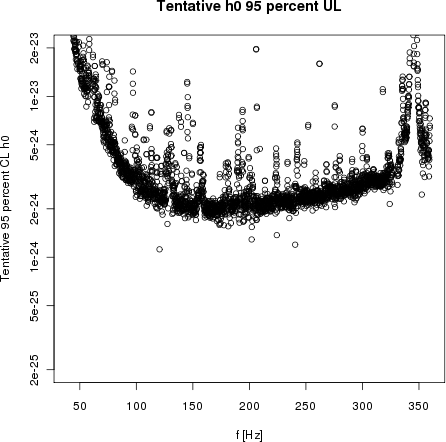
\includegraphics[width=0.5\paperwidth,height=0.4\paperheight]{plots/h0FullUL95logGuess-L1.png}}


\author{Grant David Meadors}


%\institute{\emph{
\includegraphics[height=0.3cm, width=1.1cm]{plots/michigan.png}
%U. of Michigan, Ann Arbor}}


\date{2014 October 24
\includegraphics[height=0.3cm, width=1.6cm]{plots/michigan.png}}

\makebeamertitle

%\lyxframeend{}\lyxframe{Table of Contents}
%
%\tableofcontents{}
%
%\note[item]{Near term: direct binary searches toward promising targets}
%\note[item]{Long term: enhance all searches, start age of astronomy}
%\note[item]{TwoSpect binary searches -- directed, Sco X-1}

\lyxframeend{}\section{Gravitational wave observatories}

\lyxframeend{}\lyxframe{Observing beyond light}

\begin{definition}
Gravitational wave observatory: 
a detector designed and built to transduce (\textit{see} or \textit{hear} depending on metaphor) ripples, in the curvature of space, emanating from movements of massive astronomical bodies
\end{definition}

\begin{figure}
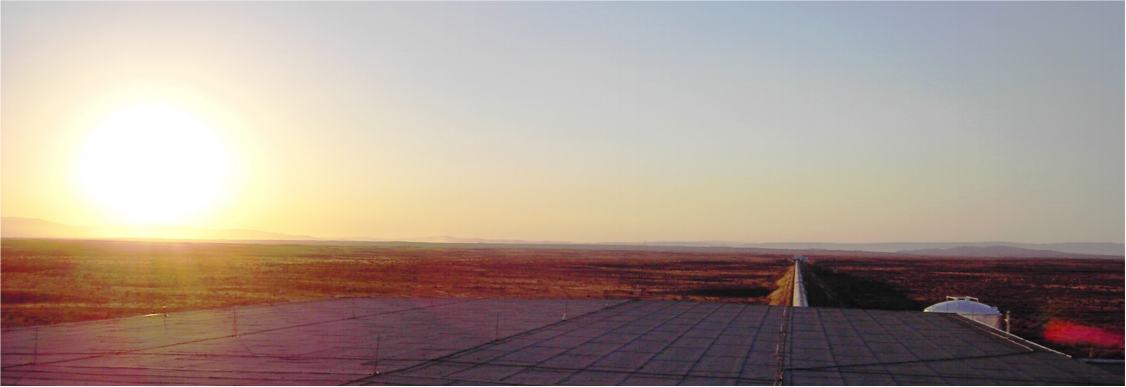
\includegraphics[width = 0.85\paperwidth]{plots/LIGOpanoramasmall}
\caption{Sunset on first-generation detectors: LIGO Hanford Observatory}
\end{figure}

\lyxframeend{}\lyxframe{Observing beyond light}

\textbf{Questions that gravitational waves answer}
\begin{exampleblock}{}
{\large How does the fabric of the universe \textit{change?}}\newline
--How does gravity change?\newline
$\textup{    }$(e.g., how soon would we stop orbiting the Sun if it vanished?)\newline
--Does gravity not travel instantaneously?\newline
--Can ripples of \textit{gravity's travel} be sensed?
\end{exampleblock}

\lyxframeend{}\lyxframe{Observing beyond light}

\textbf{General relativity}: universe extremizes \textit{curvature} $R$,\newline
constrained by \textit{cosmological constant} $\Lambda$ and \textit{matter} $\mathcal{L}_M$,
measured by \textit{metric} $g$:

\[
0 = \delta \int \left(\frac{1}{8\pi}(R - 2 \Lambda) + \mathcal{L}_M \right) \sqrt{-|g|}d^4 x,
\]

implies the Einstein field equations, with stress-energy tensor $T$:

\[
R_{\mu\nu} - \frac{1}{2} g_{\mu\nu} (R + 2\Lambda) = 8\pi T_{\mu\nu},
\]

which simplify to a \textbf{wave equation}\newline
when $g_{\mu\nu} = \eta_{\mu\nu} + h_{\mu\nu}$,\newline
for flat space $\eta$ and a small wave $h$:

\[
-\frac{1}{2} \partial_t^2 h_{\mu\nu} = 8\pi T_{\mu\nu}.
\]

\lyxframeend{}\lyxframe{Observing beyond light}

\textbf{Wave equation} on last page is sourced by $T$:
\begin{itemize} 
\item Conservation of mass-energy $\rightarrow$ no monopole radiation
\item Conservation of momentum $\rightarrow$ no dipole (unlike light)
\item Quadrupoles (\& higher) needed: \textbf{massive} astrophysical bodies
\end{itemize}

Traveling spatial distortion, direction $k_\mu$, \newline
2 polarizations ($h_+$ \& $h_\times$):

\[
h_{\mu\nu} =
\left[
\begin{array}{cccc}
0 & 0 & 0 & 0\\
0 & -h_+ & h_\times & 0 \\
0 & h_\times & h_+ & 0\\
0 & 0 & 0 & 0
\end{array} \right] \Re \left(e^{\sqrt{-1} (k_\mu x^\mu + \phi_0)} \right).
\]

Meaning space itself `stretches' in one direction, then another

\lyxframeend{}\lyxframe{Observing beyond light}

%What kind of massive astrophysical bodies?

\begin{figure}
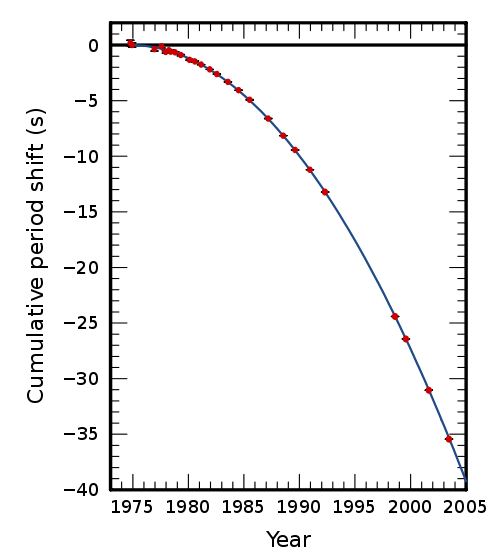
\includegraphics[width=0.4\paperwidth]{plots/500px-PSR_B1913+16_period_shift_graph.png}
\caption{\textit{What kinds of astrophysical bodies?} PSR 1913+16 (Hulse \& Taylor): neutron star orbital decay, energy lost to gravitational waves}
\end{figure}

\lyxframeend{}\lyxframe{Observing beyond light}

Some of the most elusive phenomena in the universe should emit gravitational waves:
\begin{table}[t]
\begin{tabular}{c | cc}
& transient events & long-lasting \\
\hline \\
predicted form & inspirals & pulsars \\
unknown form & bursts & stochastic 
\end{tabular}
\end{table}

\begin{description}
\item [{Inspirals}] of merging neutron stars \& black holes
\item [{Pulsars}] with mountains on neutron (quark?) crust
\item [{Bursts}] from supernovae, hypernovae (GRBs)...
\item [{Stochastic}] background of the Big Bang, white dwarf stars...
\end{description}

\lyxframeend{}\section{Making observatories small \& large}
\lyxframeend{}\lyxframe{Making observatories small \& large}

\textbf{LIGO}: \textit{Laser Interferometry Gravitational-wave observatory}\newline
built to detect gravitational waves, along with collaborators in GEO600 (Germany-UK), Virgo (France-Italy), KAGRA (Japan), INDIGO (India), and many others in Australia and around the world

LIGO features:
\begin{itemize}
\item Power-recycled \textbf{Michelson interferometer} with \textbf{4 km} Fabry-Perot arms (ultra-high vacuum)
\item \textbf{Hanford, Washington} and \textbf{Livington, Louisiana} observatories
%\item $10^{−9}$ torr vacuum
\item \textbf{20 W} Nd:YAG 1064 nm laser (upgrading to 200 W)
\item \textbf{10 kg} fused silica primary optics (upgrading to 40 kg)
\item \textbf{4-stage} seismic isolation (upgrading to 7-stage)
\item \textbf{about 1000} scientists \& engineers
\end{itemize}

\lyxframeend{}\lyxframe{Making observatories small \& large}
\begin{figure}
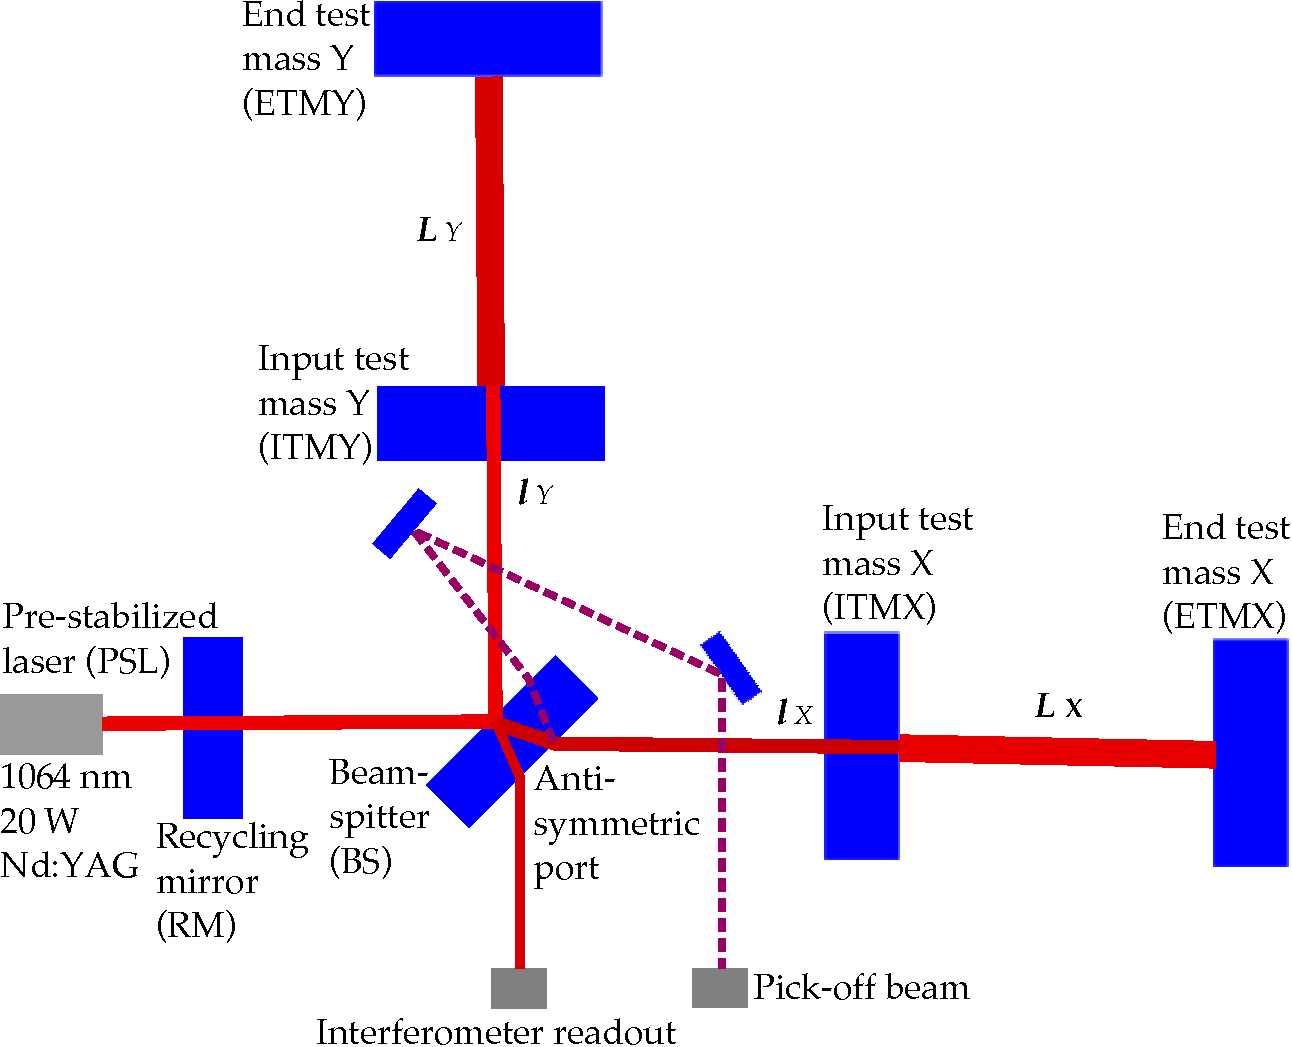
\includegraphics[width=0.6\paperwidth]{plots/figure1}
\caption{LIGO: Michelson interferometer w/ Fabry-Perot arms}
\end{figure}

\lyxframeend{}\lyxframe{Making observatories small \& large}

Gravitational wave $h_+$ changes relative phase of light in arms,\newline

\[
T_x = \int_0^{\frac{2L_x}{c}} \sqrt{|g_{xx}|} dt \approx \int_0^{\frac{2L_x}{c}} \left(1 - \frac{h_+ (t,x(t))}{2} \right) dt,
\]
\[
T_y = \int_0^{\frac{2L_y}{c}} \sqrt{|g_{yy}|} dt \approx \int_0^{\frac{2L_y}{c}} \left(1 + \frac{h_+ (t, y(t))}{2} \right) dt,
\]
\[
\phi_{\textup{DARM}} \equiv \omega (T_y - T_x) = \omega \int_0^{\frac{2L}{c}} \frac{h_+ (t, x(t)) + h_+ (t, y(t))}{2} dt.
\] 

\noindent Michelson interferometer power changes, \newline
gravitational wave (proportional to power) \textbf{observable}



\lyxframeend{}\lyxframe{Making observatories small \& large}
\textbf{Design simple models (\& exhibits)}

\begin{figure}
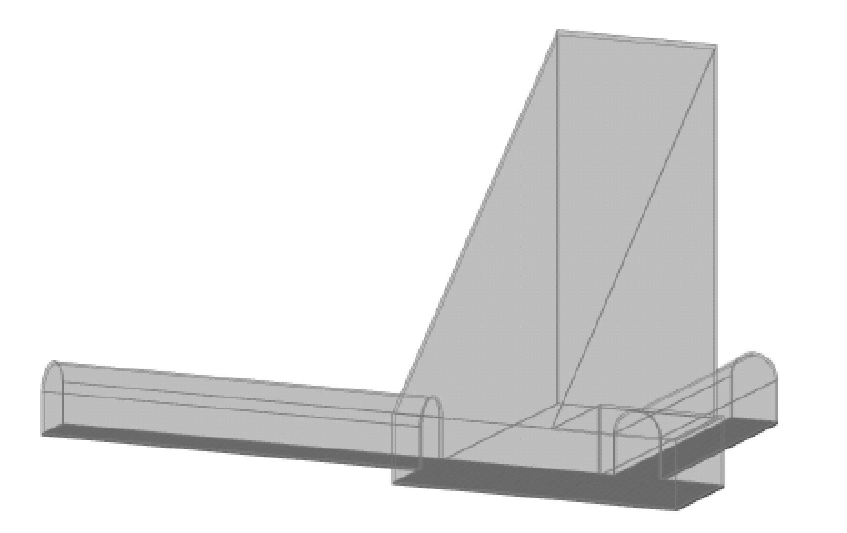
\includegraphics[width=0.4\paperwidth]{plots/view-corner.png}
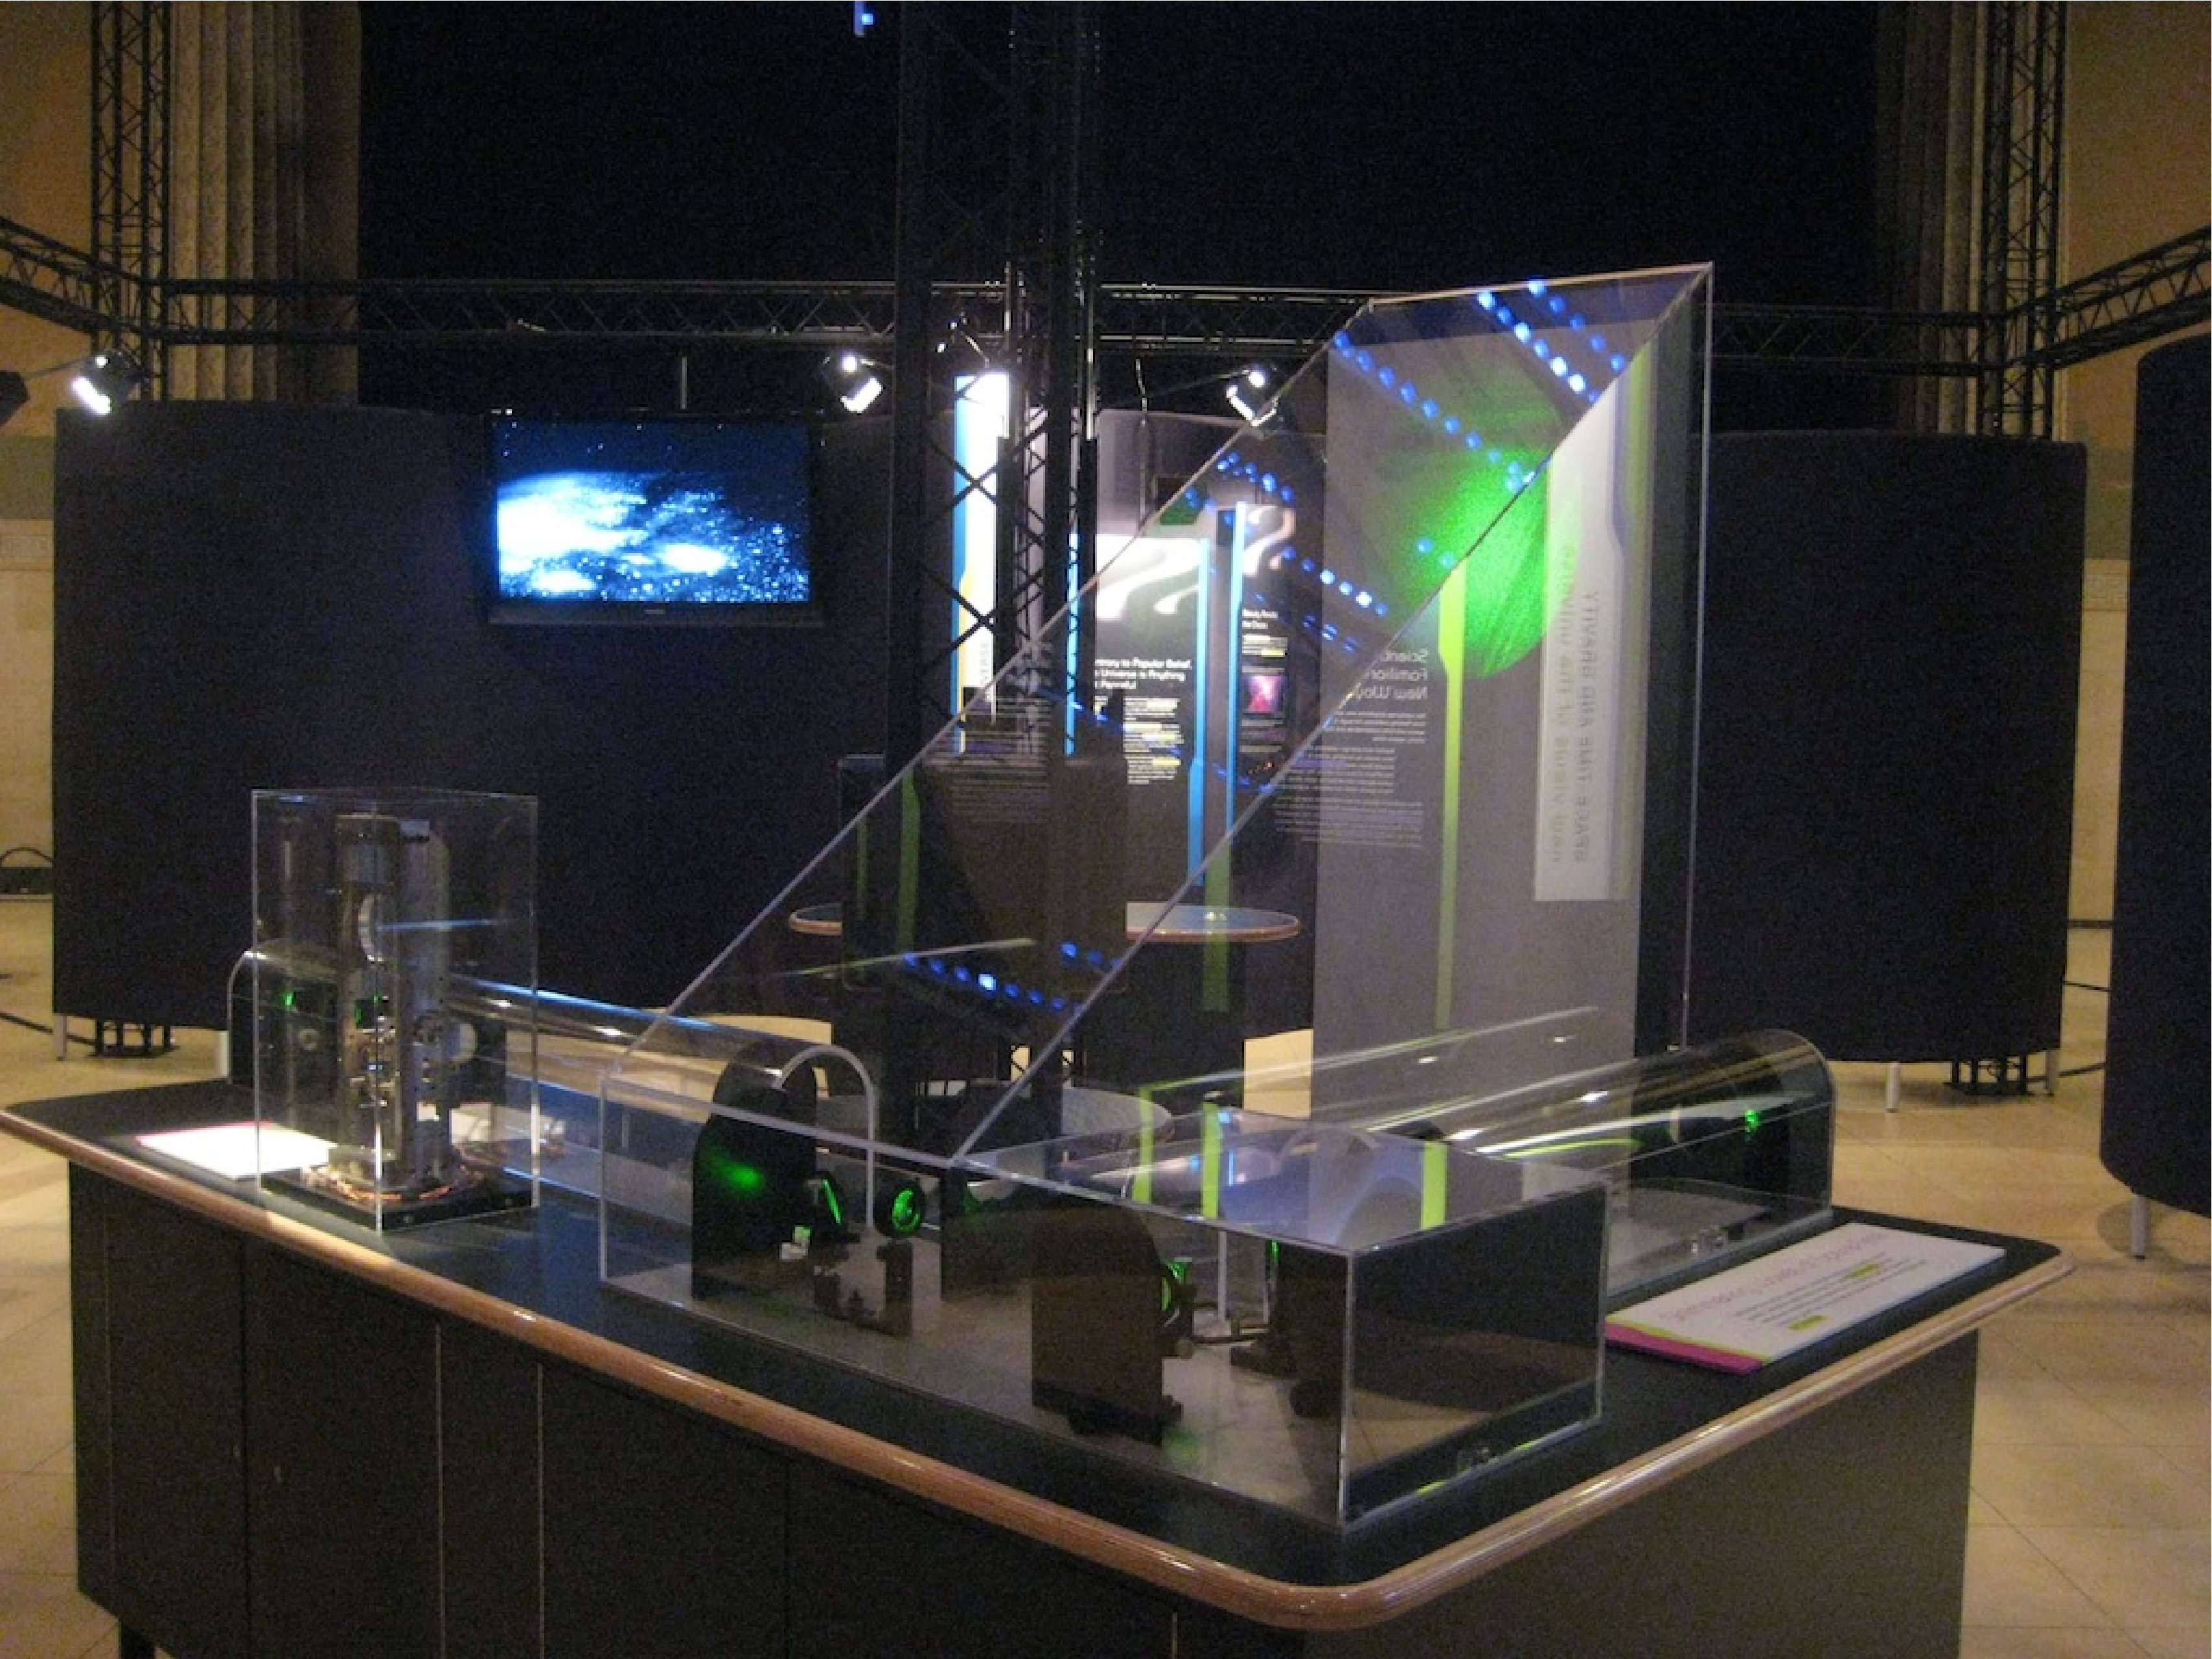
\includegraphics[width=0.4\paperwidth]{plots/WSF_in_NY.png}
\caption{World Science Festival interferometer: AutoCAD model \& as-built}
\end{figure}

\lyxframeend{}\lyxframe{Making observatories small \& large}

\textbf{Commission (hands-on)}

\begin{figure}
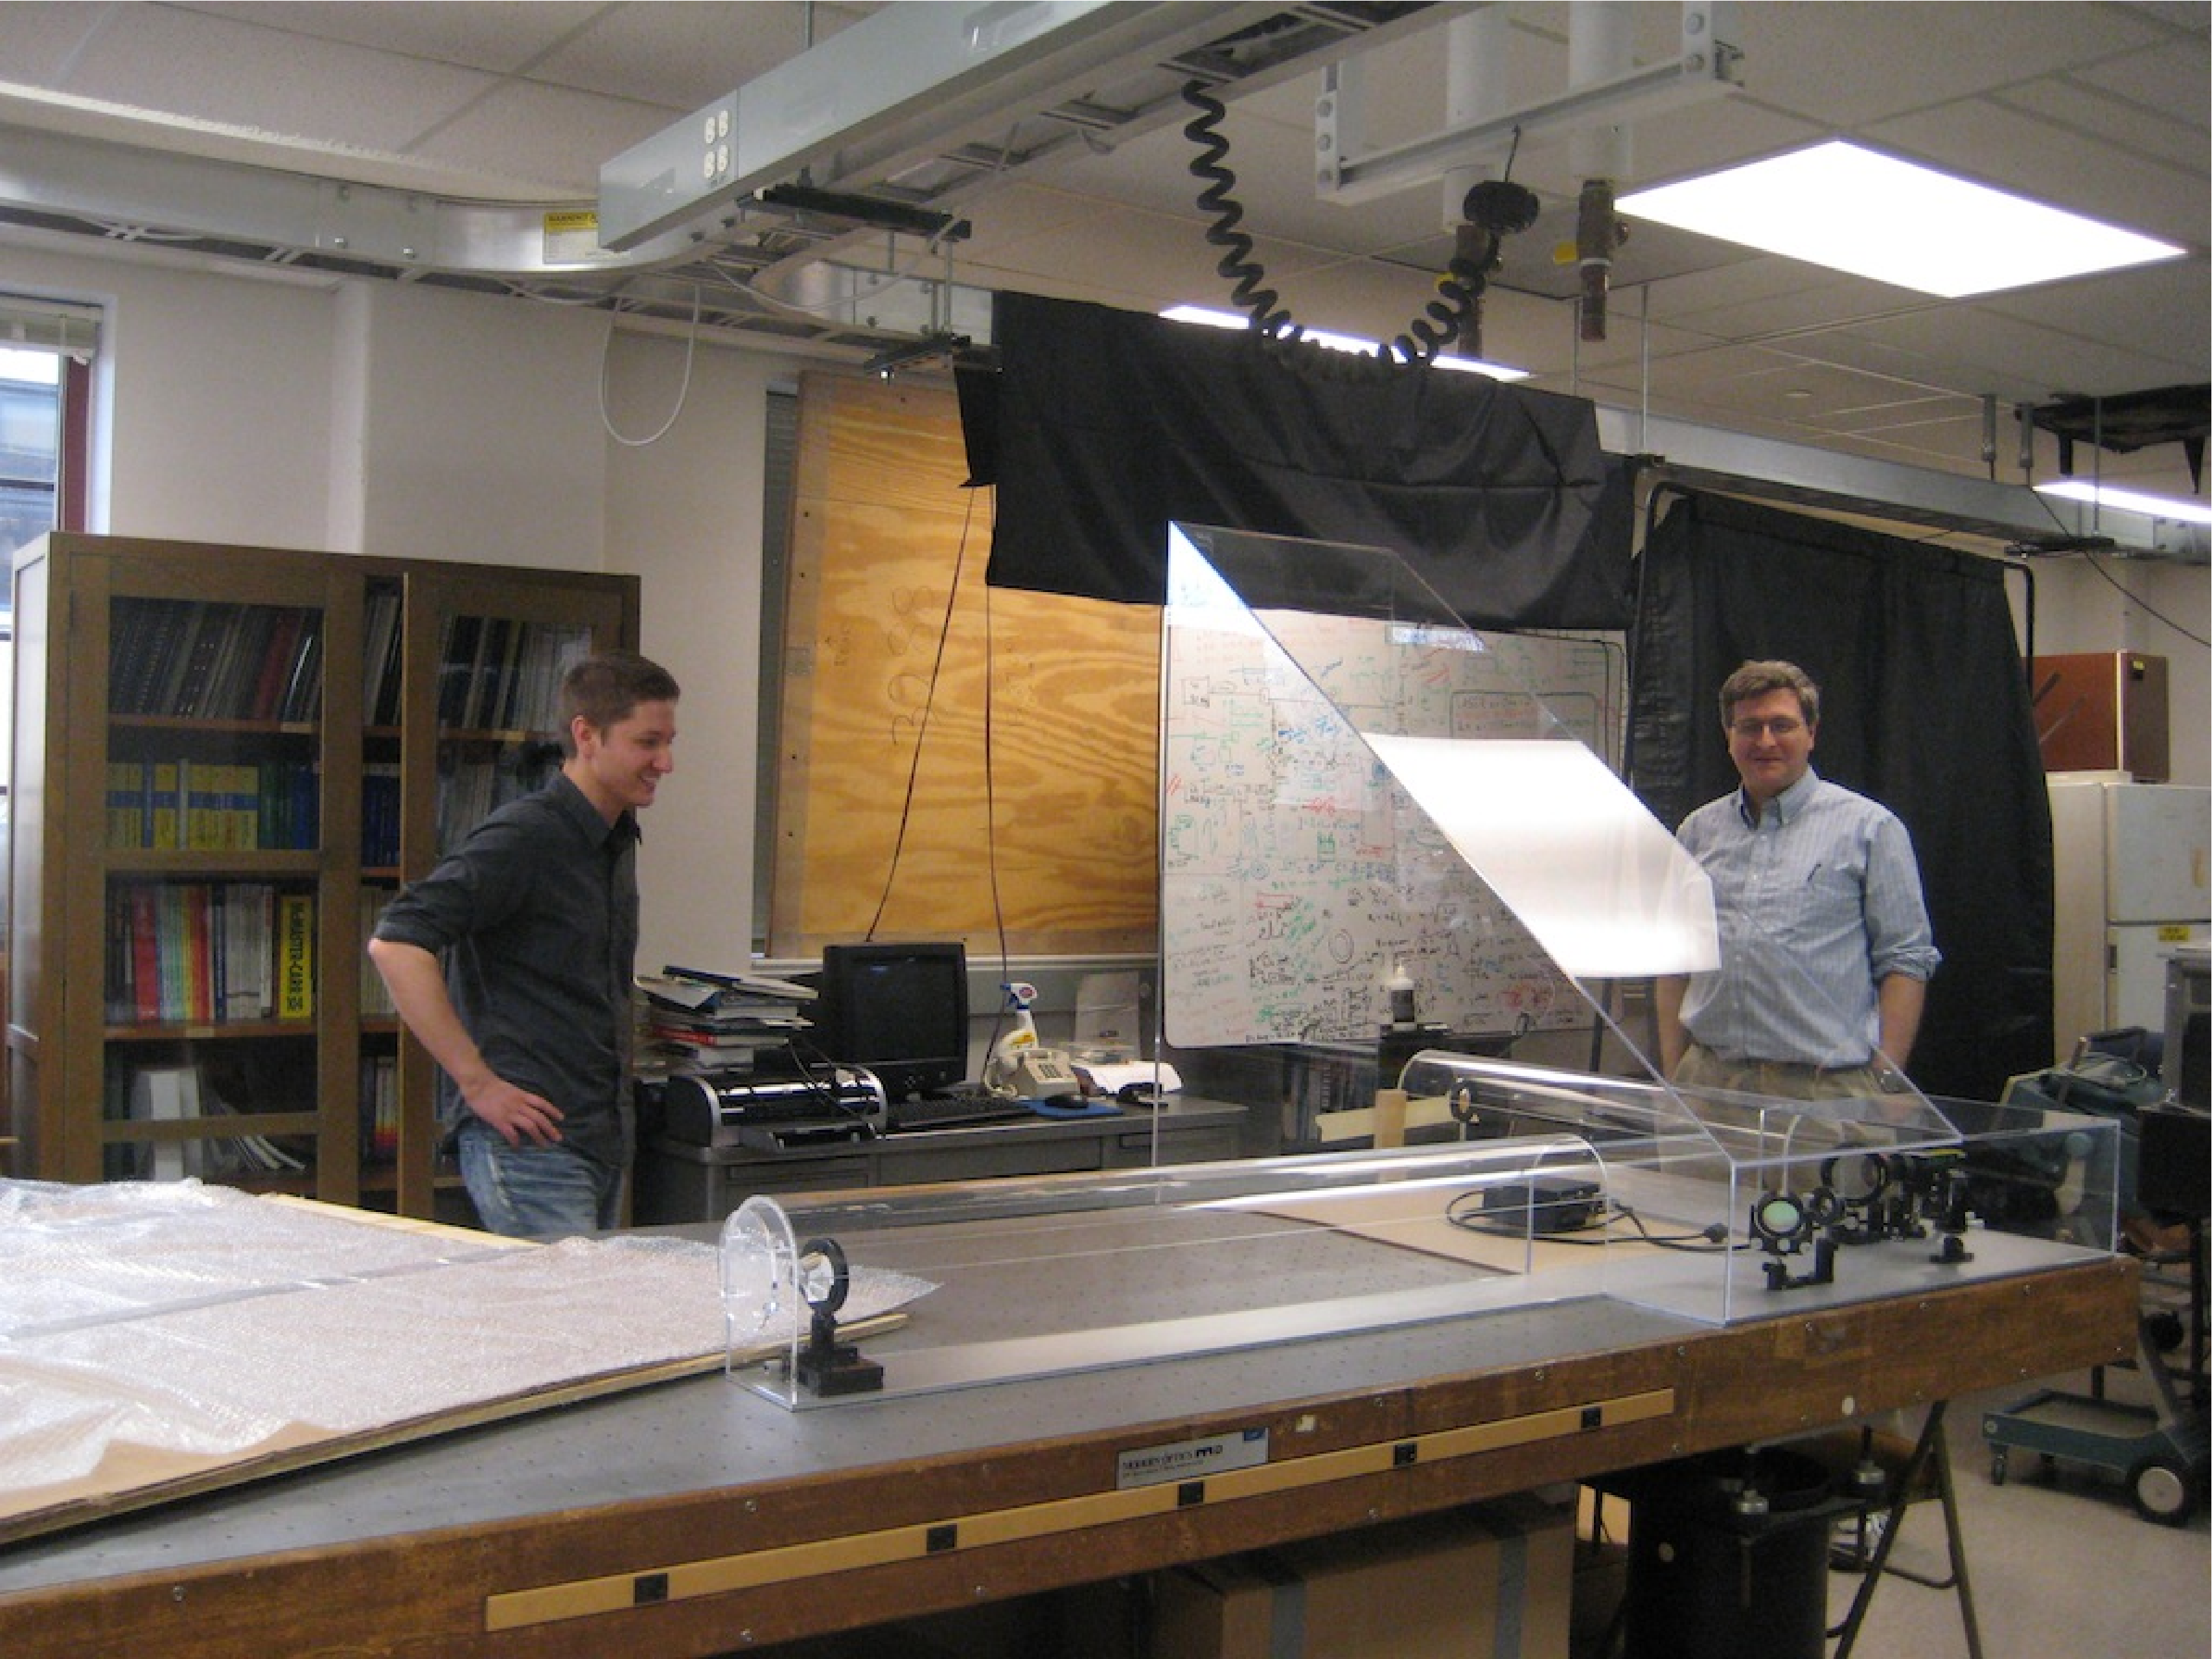
\includegraphics[width=0.4\paperwidth]{plots/WSF_under_construction.png}
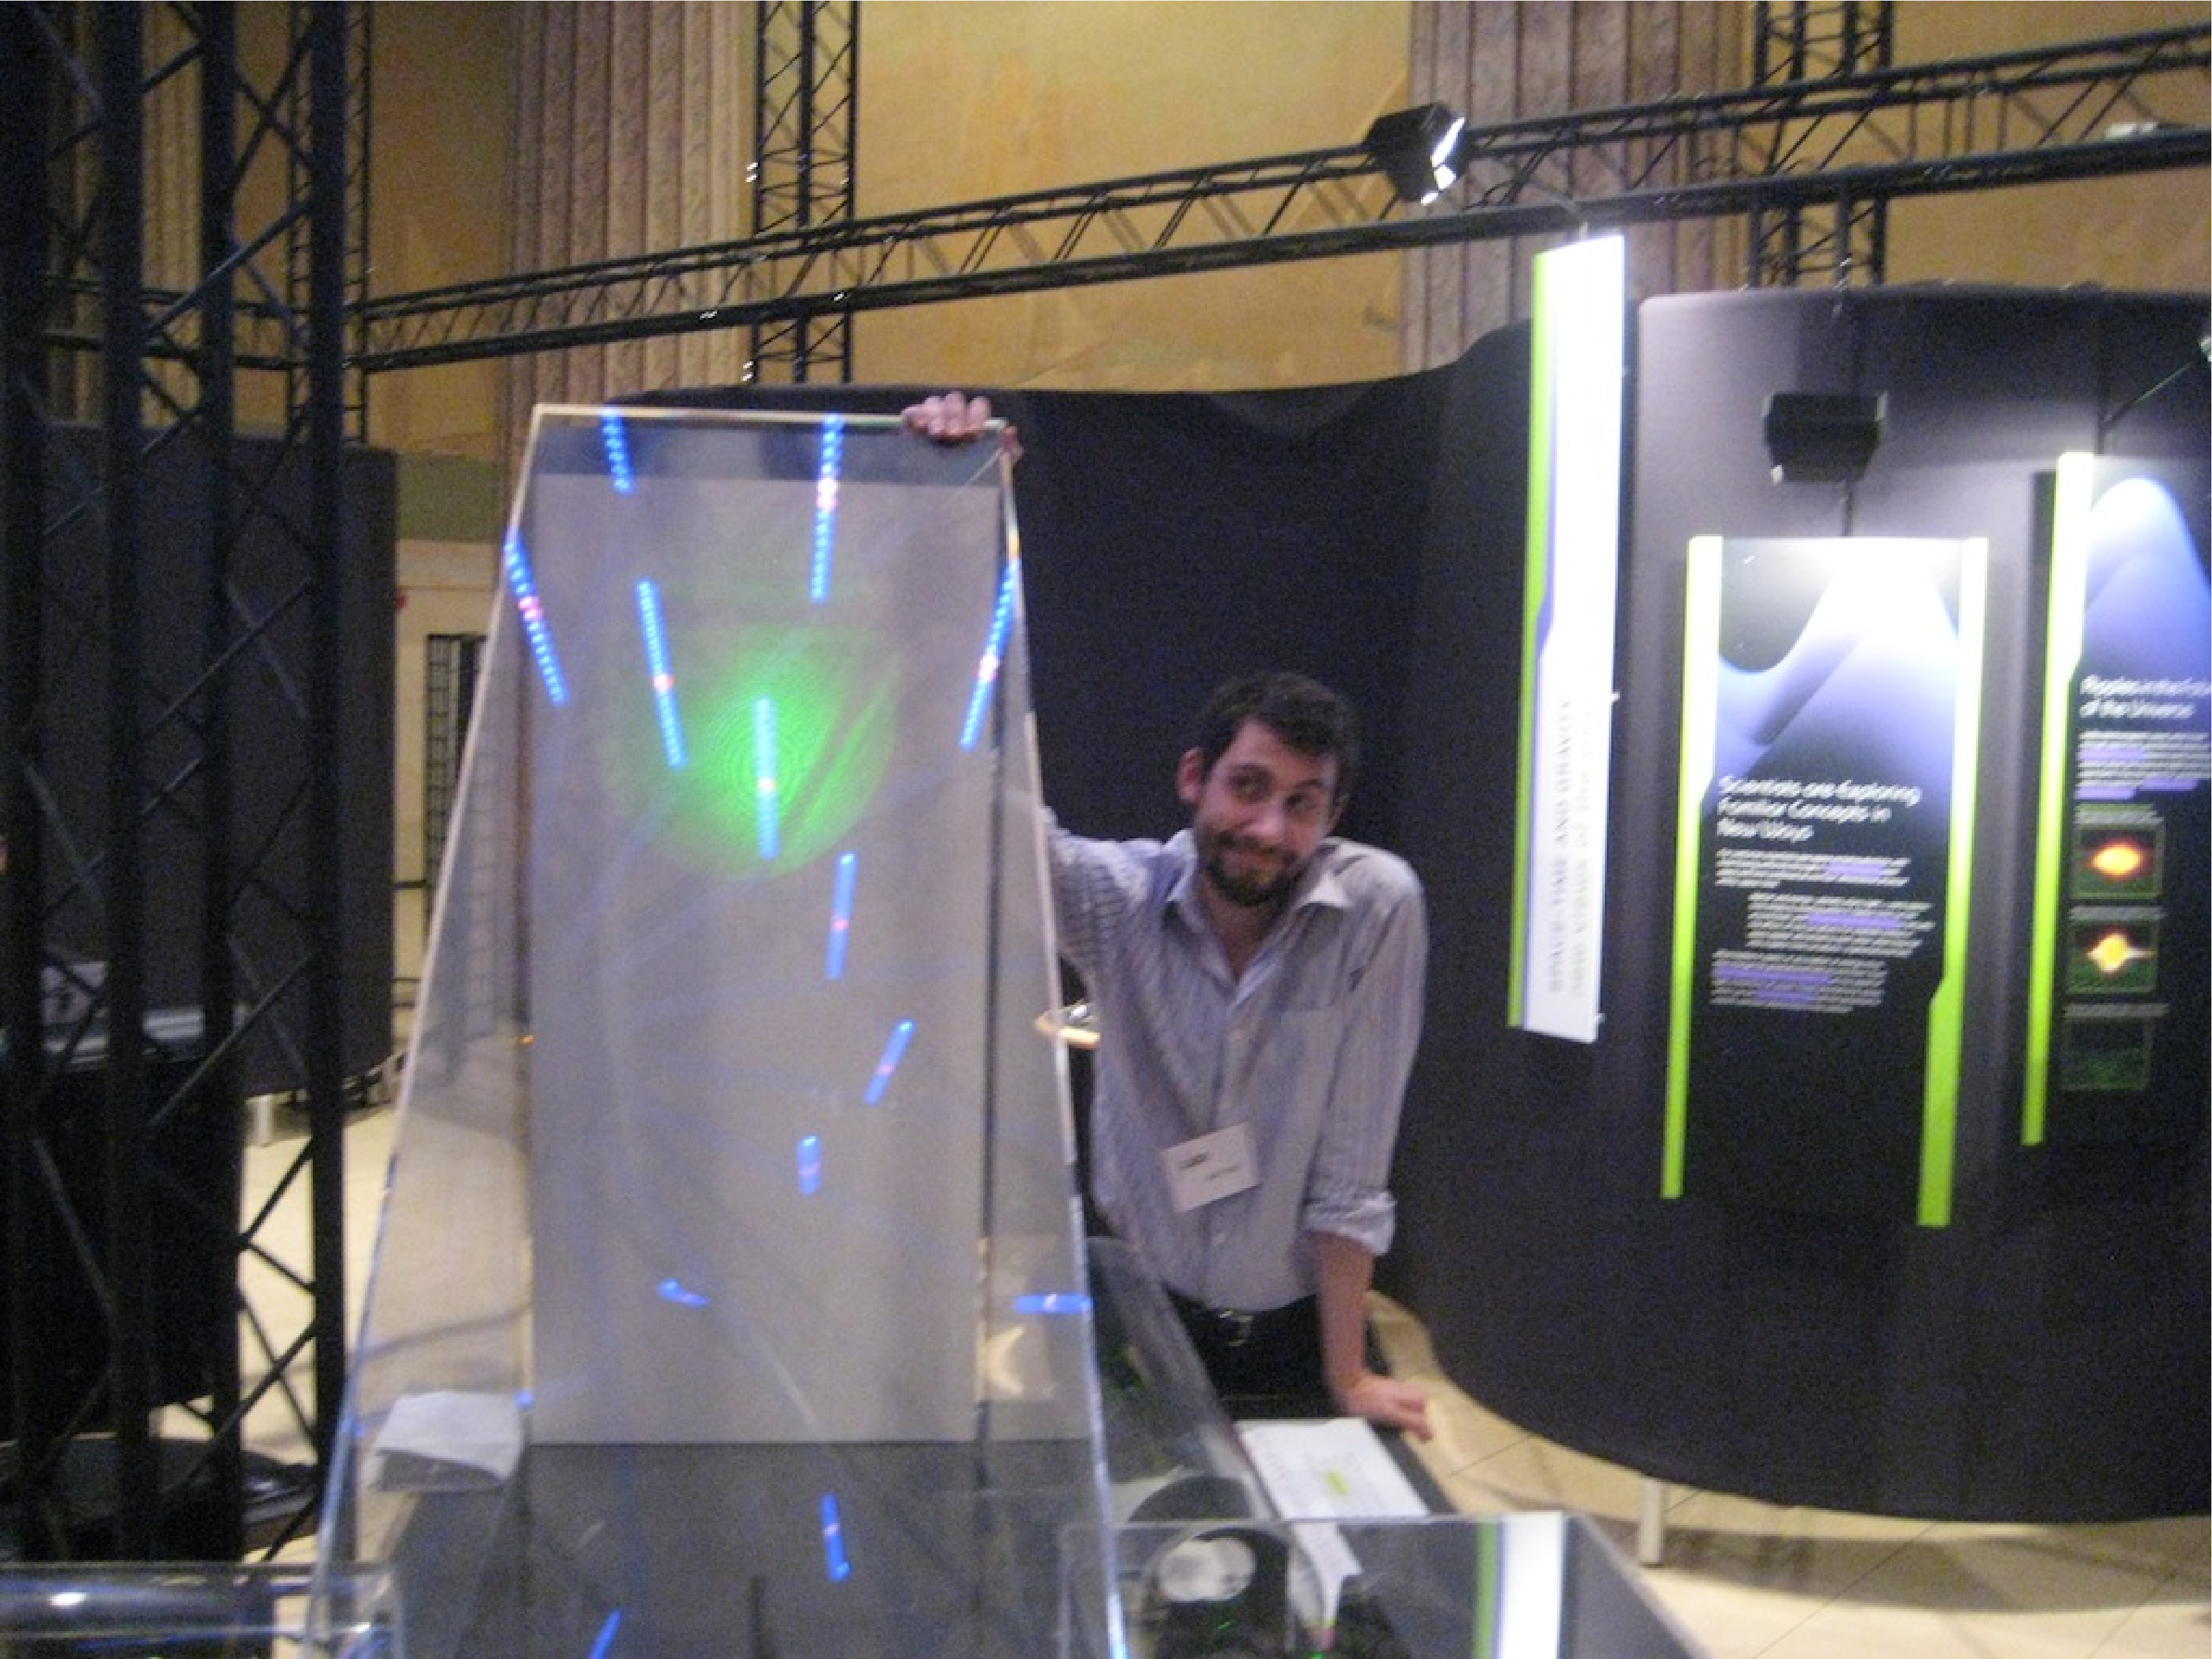
\includegraphics[width=0.4\paperwidth]{plots/WSF_me_NY.png}
\caption{Humans need to stay involved for instruments to work!}
\end{figure}






\lyxframeend{}\section{Squeezing large interferometers}


\lyxframeend{}\lyxframe{Squeezing introduction}
\begin{definition}%{}
Altering $\Delta E\Delta\phi$ uncertainty for the electromagnetic
field\end{definition}%{}
\begin{itemize}
\item Demonstrated first at GEO 600, then LIGO Hanford (H1)\end{itemize}
\begin{theorem}%{}
Shot noise arises from quantum operators (Caves 1980, 1981)\end{theorem}%{}
\begin{itemize}
\item Vacuum fluctuations couple through anti-symmetric port
\item \emph{Squeeze }the $\overrightarrow{E}$ field uncertainty ellipse
\item Angle $\theta$, factor $r$, creation operator $a$, squeeze operator
$S$:
\end{itemize}
\[
S(\zeta)=\exp[\frac{1}{2}\zeta^{*}a^{2}-\frac{1}{2}\zeta(a^{\dagger})^{2}],\;\zeta=re^{i\theta}
\]


Squeezed state made with

optical parameter oscillator, 2nd harmonic generator

\textbf{Shot noise reduced by $e^{-r}$}

\[
\]



\lyxframeend{}\lyxframe{Squeezing large interferometers}

\begin{figure}
\caption{\protect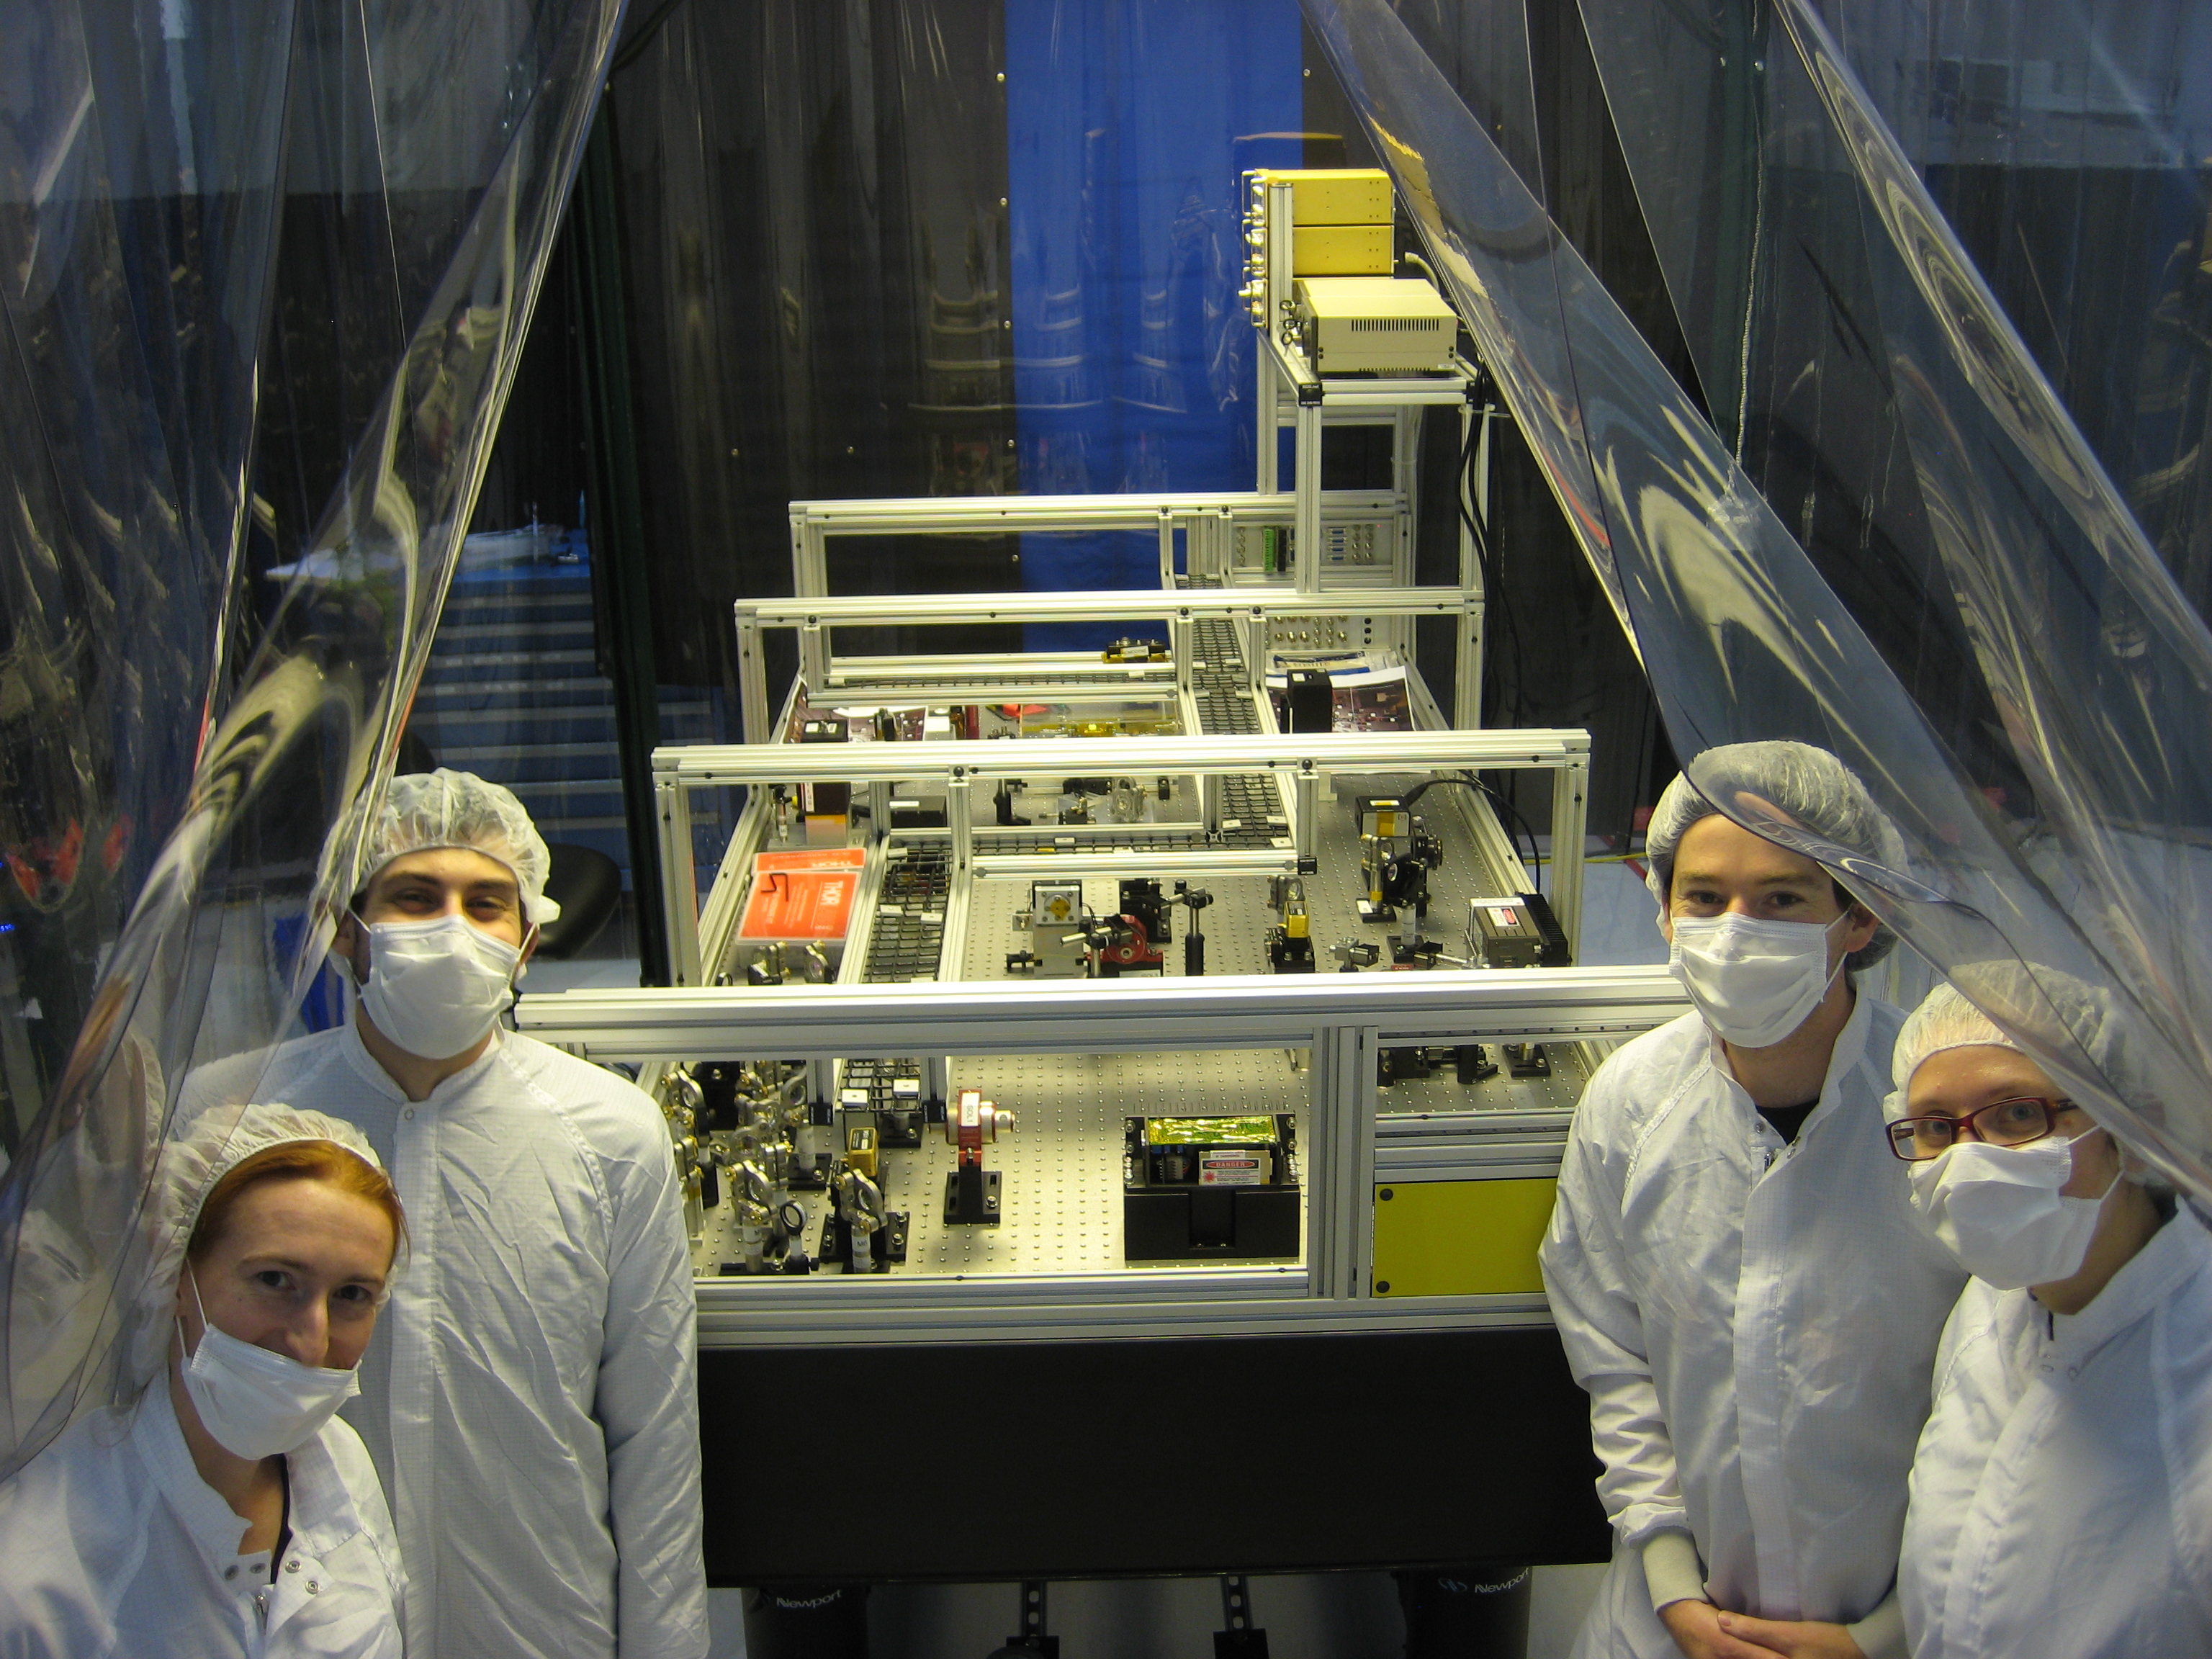
\includegraphics[width=0.33\paperwidth]{plots/lisabar-1289966130}}


\caption{\protect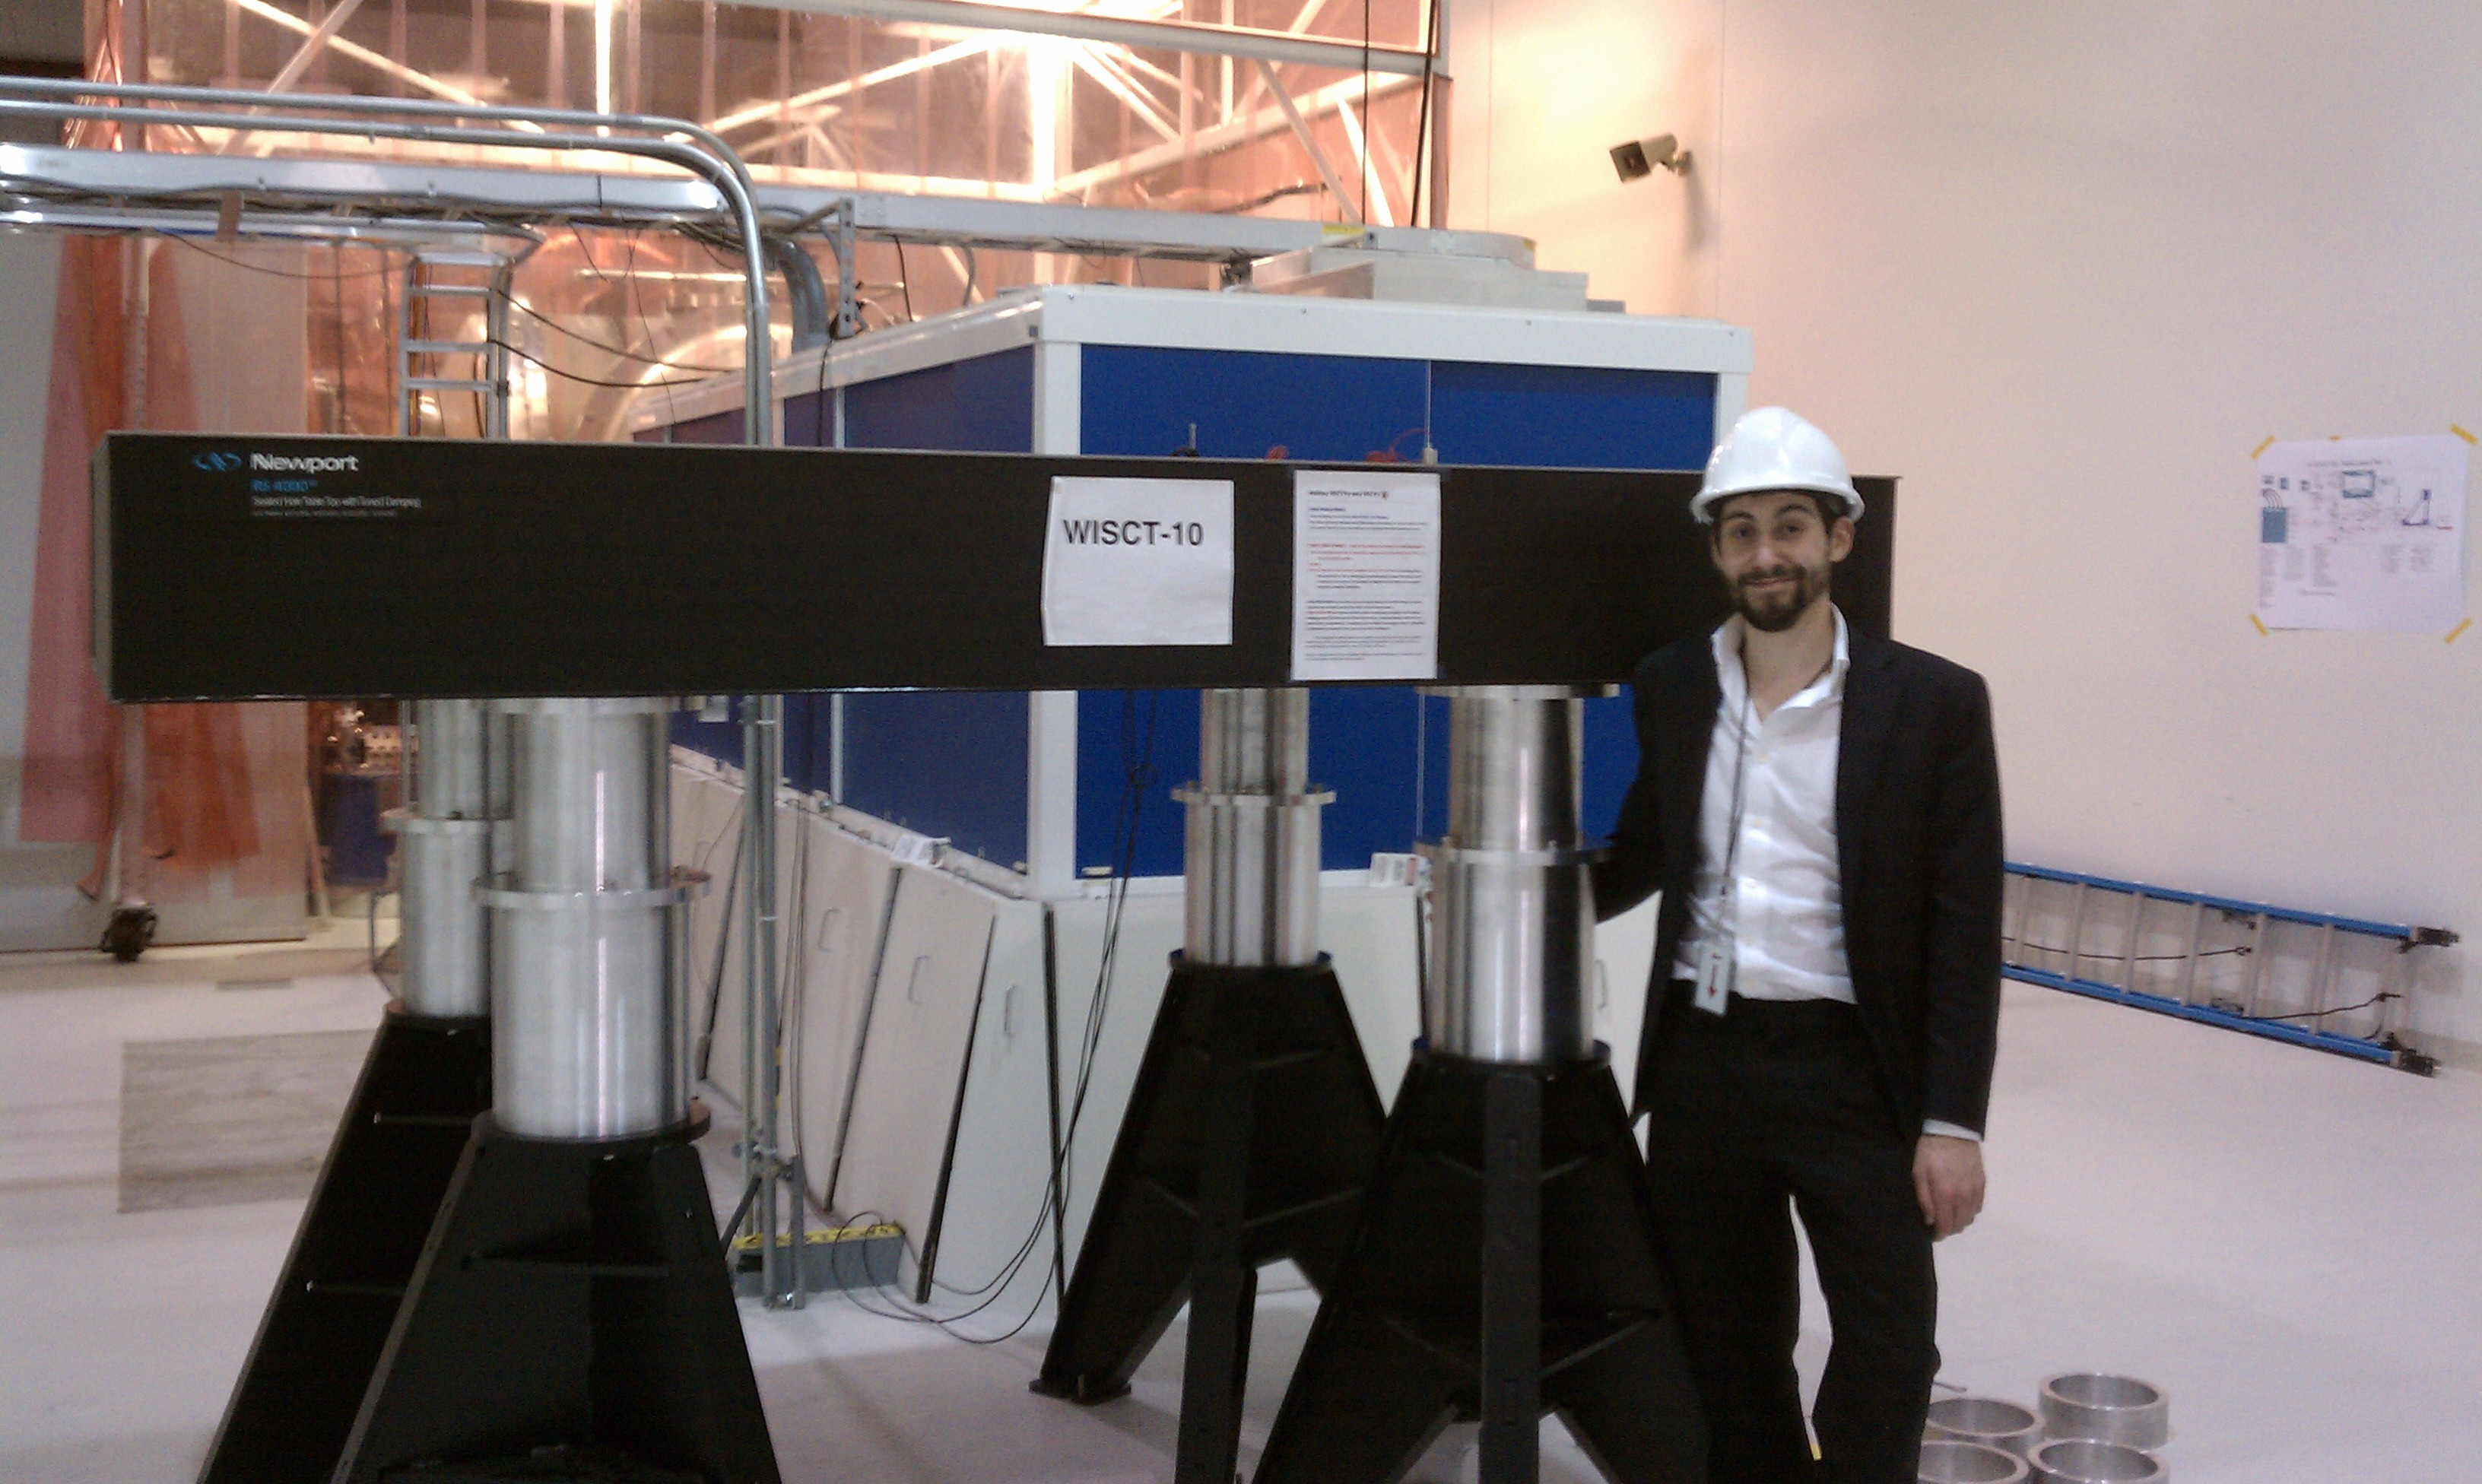
\includegraphics[width=0.33\paperwidth]{plots/lisabar-1300943141}}


Images by Lisa Barsotti in Hanford eLog

TOP: CC from LL, Dwyer, Barsotti, Mow-Lowry, Meadors

BOTTOM: table legs (\& helped w/ Faraday isolator, data channels)
\end{figure}



\lyxframeend{}\lyxframe{Squeezing's scientific benefit}

\begin{figure}
\caption{\protect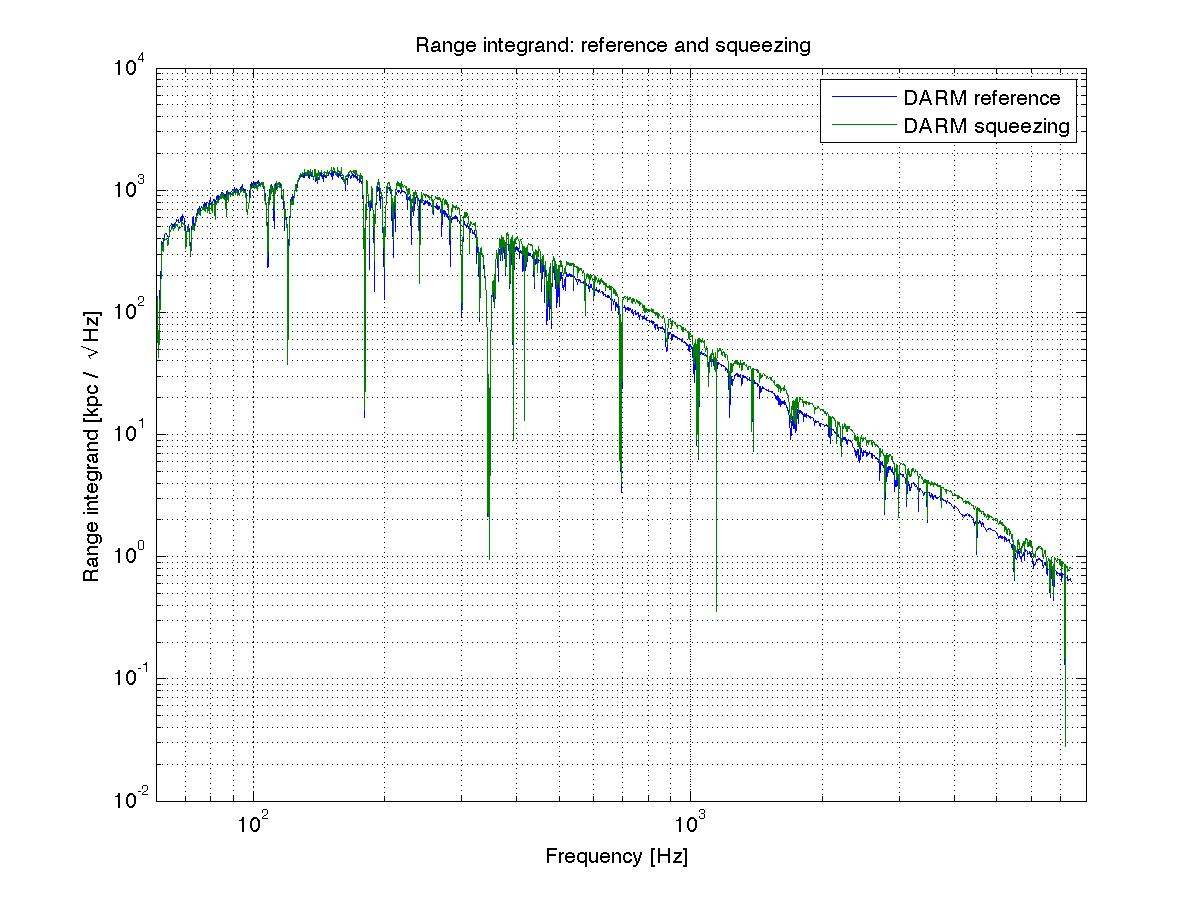
\includegraphics[width=0.45\paperwidth,height=0.45\paperheight,keepaspectratio]{plots/range_integrand.jpeg}\protect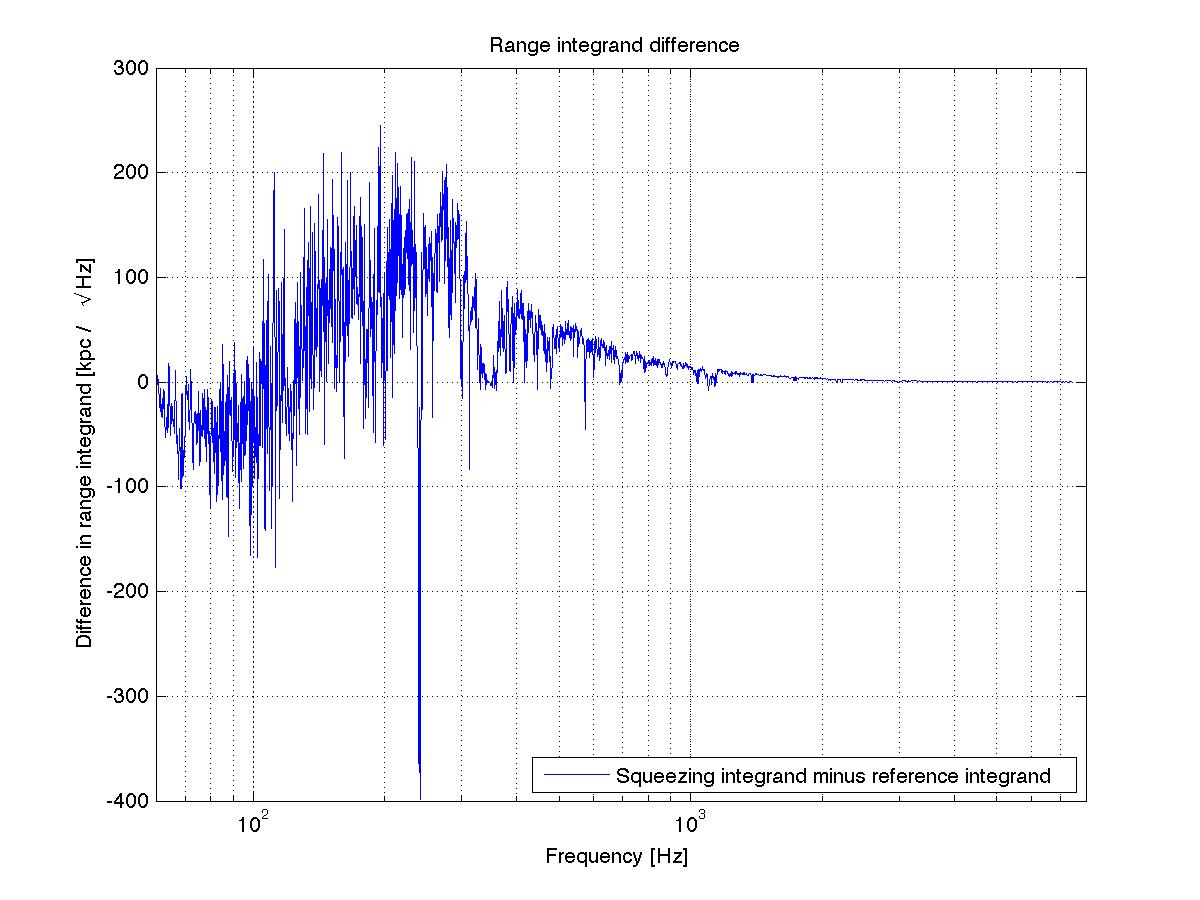
\includegraphics[width=0.45\paperwidth,height=0.45\paperheight,keepaspectratio]{plots/range_integrand_difference.jpeg}}


LEFT: integrand of inspiral range as a function of frequency

RIGHT: net effect of squeezing on inspiral range integrand

Scientific benefit at few hundred Hz $\rightarrow$ all ways to improve
are good
\end{figure}



\lyxframeend{}\lyxframe{Squeezing summary}
\begin{description}
\item [{Instrumental}] experience with technique important beyond Advanced
LIGO
\item [{Physical}] way to improve broad band of LIGO, benefit many searches
\item [{Illustrates}] need for best sensitivity at few hundred Hz
\item [{Question}] what can we improve \emph{post-facto?}
\end{description}

\lyxframeend{}\section{Auxiliary length control noise}


\lyxframeend{}\subsection*{LIGO}


\lyxframeend{}\lyxframe{LIGO}
\begin{onlyenv}%{}
<1>
\end{onlyenv}%{}
MICH noise seen as DARM/(arm gain); PRC too seen in DARM
\begin{columns}%{}
\column{5cm}

\[
\begin{array}{c}
CARM\\
\textrm{common arm}
\end{array}=L_{+}=\frac{\delta(L_{y}+L_{x})}{2}
\]


\[
\begin{array}{c}
DARM\\
\textrm{differential arm}
\end{array}=L_{-}=\delta(L_{y}-L_{x})
\]


\[
\begin{array}{c}
PRC\\
\textrm{power-recycling cavity}
\end{array}=l_{+}=\frac{\delta(l_{y}+l_{x})}{2}
\]


\[
\begin{array}{c}
MICH\\
\textrm{inner Michelson}
\end{array}=l_{-}=\delta(l_{y}-l_{x})
\]


\column{5cm}

\begin{figure}
\caption{\protect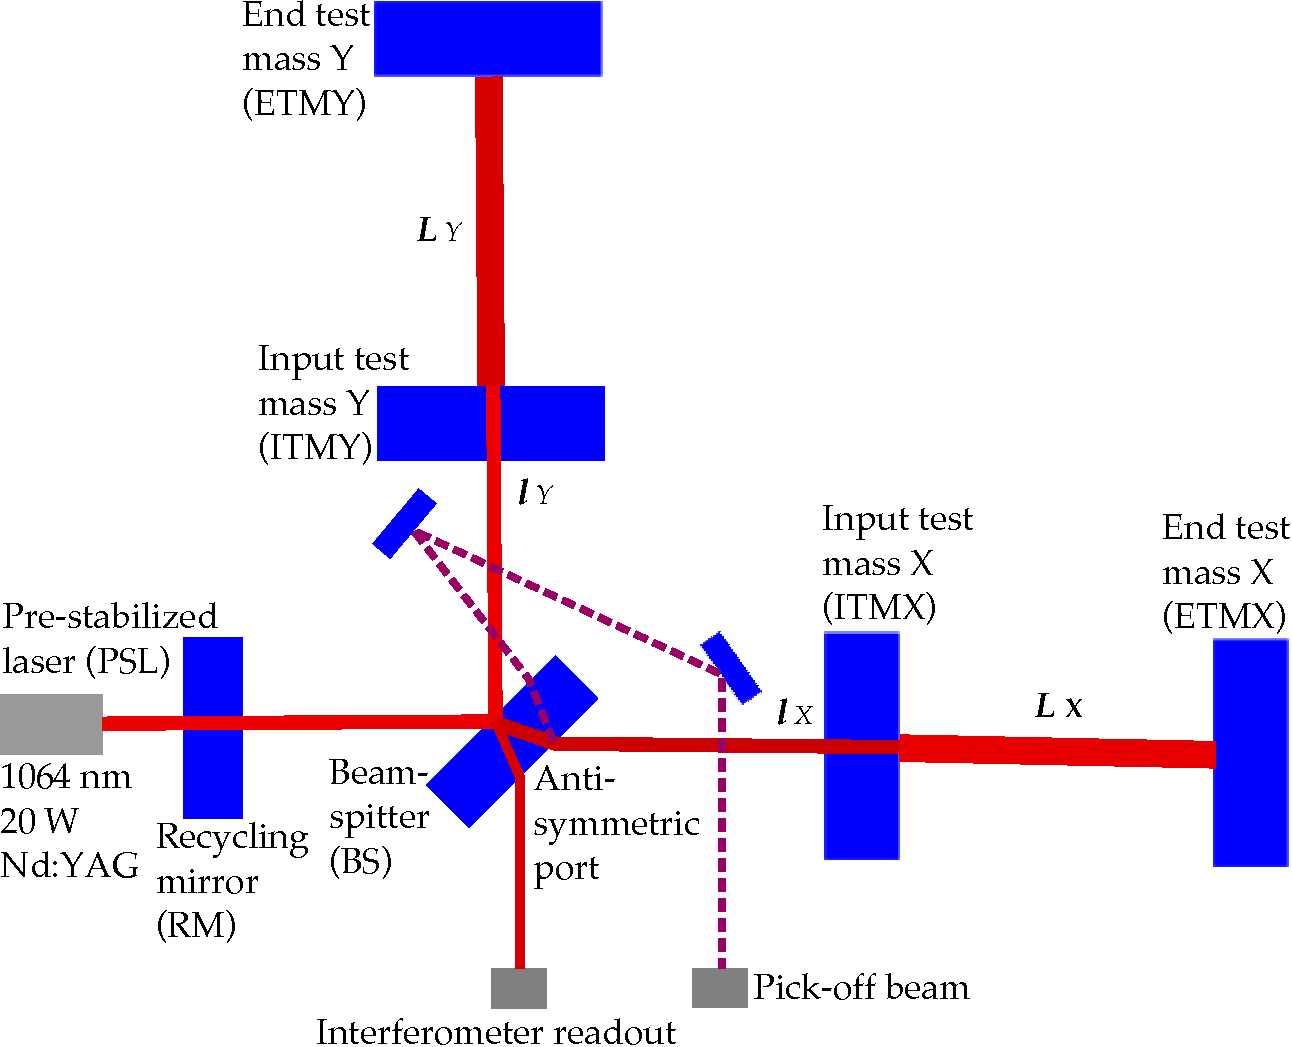
\includegraphics[width=0.95\columnwidth,height=0.4\paperheight]{plots/figure1}}
\end{figure}


$L_{y}\equiv z(ETMY)-z(ITMY)$

$L_{x}\equiv z(ETMX)-z(ITMX)$

$l_{y}\equiv z(ITMY)-z(RM)$

$l_{x}=z(ITMX)-z(RM)$
\end{columns}%{}

\lyxframeend{}\lyxframe{Problems with auxiliary length control}
\begin{itemize}
\item LIGO optical cavity lengths actively controlled
\item DARM most important; CARM, MICH, PRC auxiliary
\item MICH \& PRC: high sensing noise (low light on sensors)
\end{itemize}
$\rightarrow$cross-talk DARM predicted, seen

$\rightarrow$contaminates most sensitive band: \emph{should remove
noise}
\begin{itemize}
\item \textbf{Frequency-domain method (Allen, Hua, Ottewill, 1999)}
\item Code derived from real-time servo filter designs
\end{itemize}


\lyxframeend{}\subsection*{MICH \& PRC filtering for h(t)}


\lyxframeend{}\lyxframe{MICH \& PRC filtering for h(t)}
\begin{onlyenv}%{}
<1>

\begin{figure}
\caption{\protect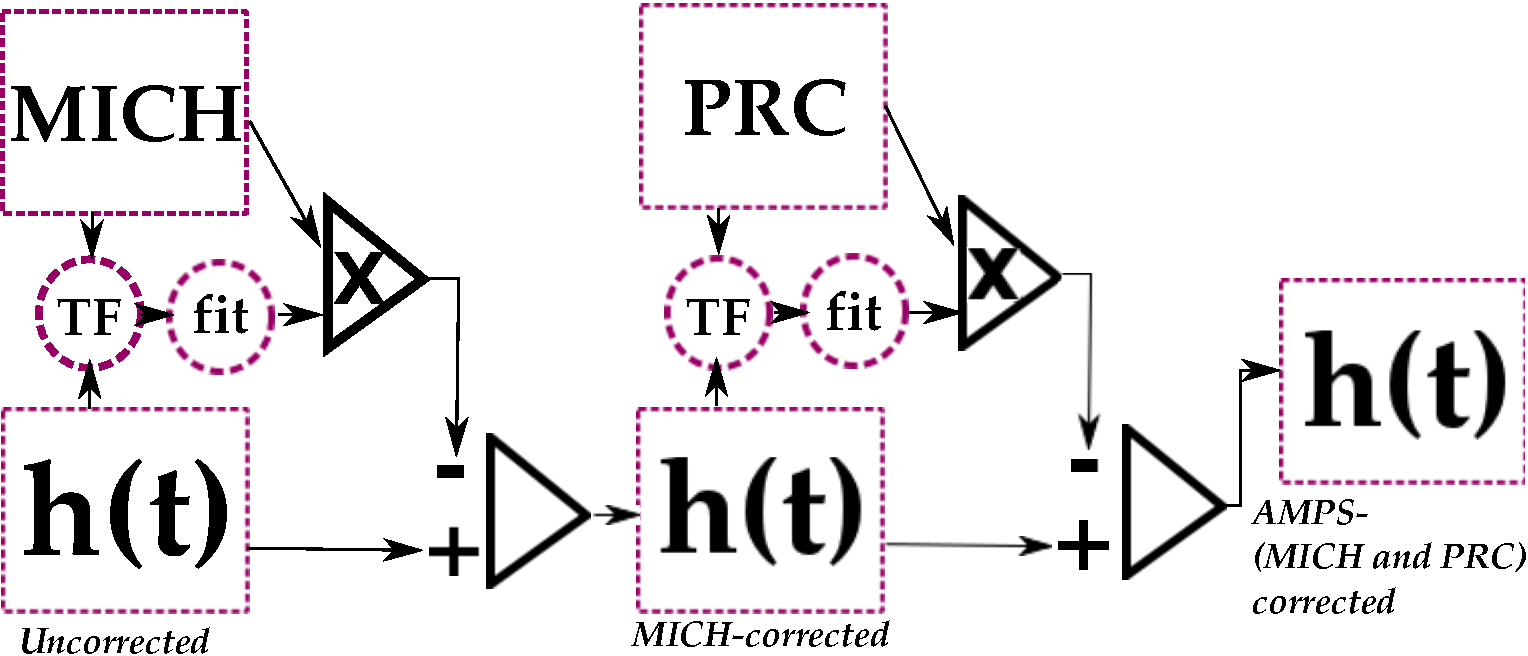
\includegraphics[width=0.9\paperwidth]{plots/figure9}}


\emph{Feedforward filtering pipeline} 

read in h(t), MICH, PRC, write 1024 of clean signal$\hat{s}(t)$

$\hat{s}(t)=\{s+\Sigma_{j}(\gamma_{j}\times n_{j})\}(t)-\Sigma_{j}(g_{j}(t)\times\{n_{j}\}(t))$

\url{matapps/packages/detchar/AMPS/trunk/aletheia.m}
\end{figure}

\end{onlyenv}%{}

\begin{onlyenv}%{}
<2>

\begin{figure}
\caption{\protect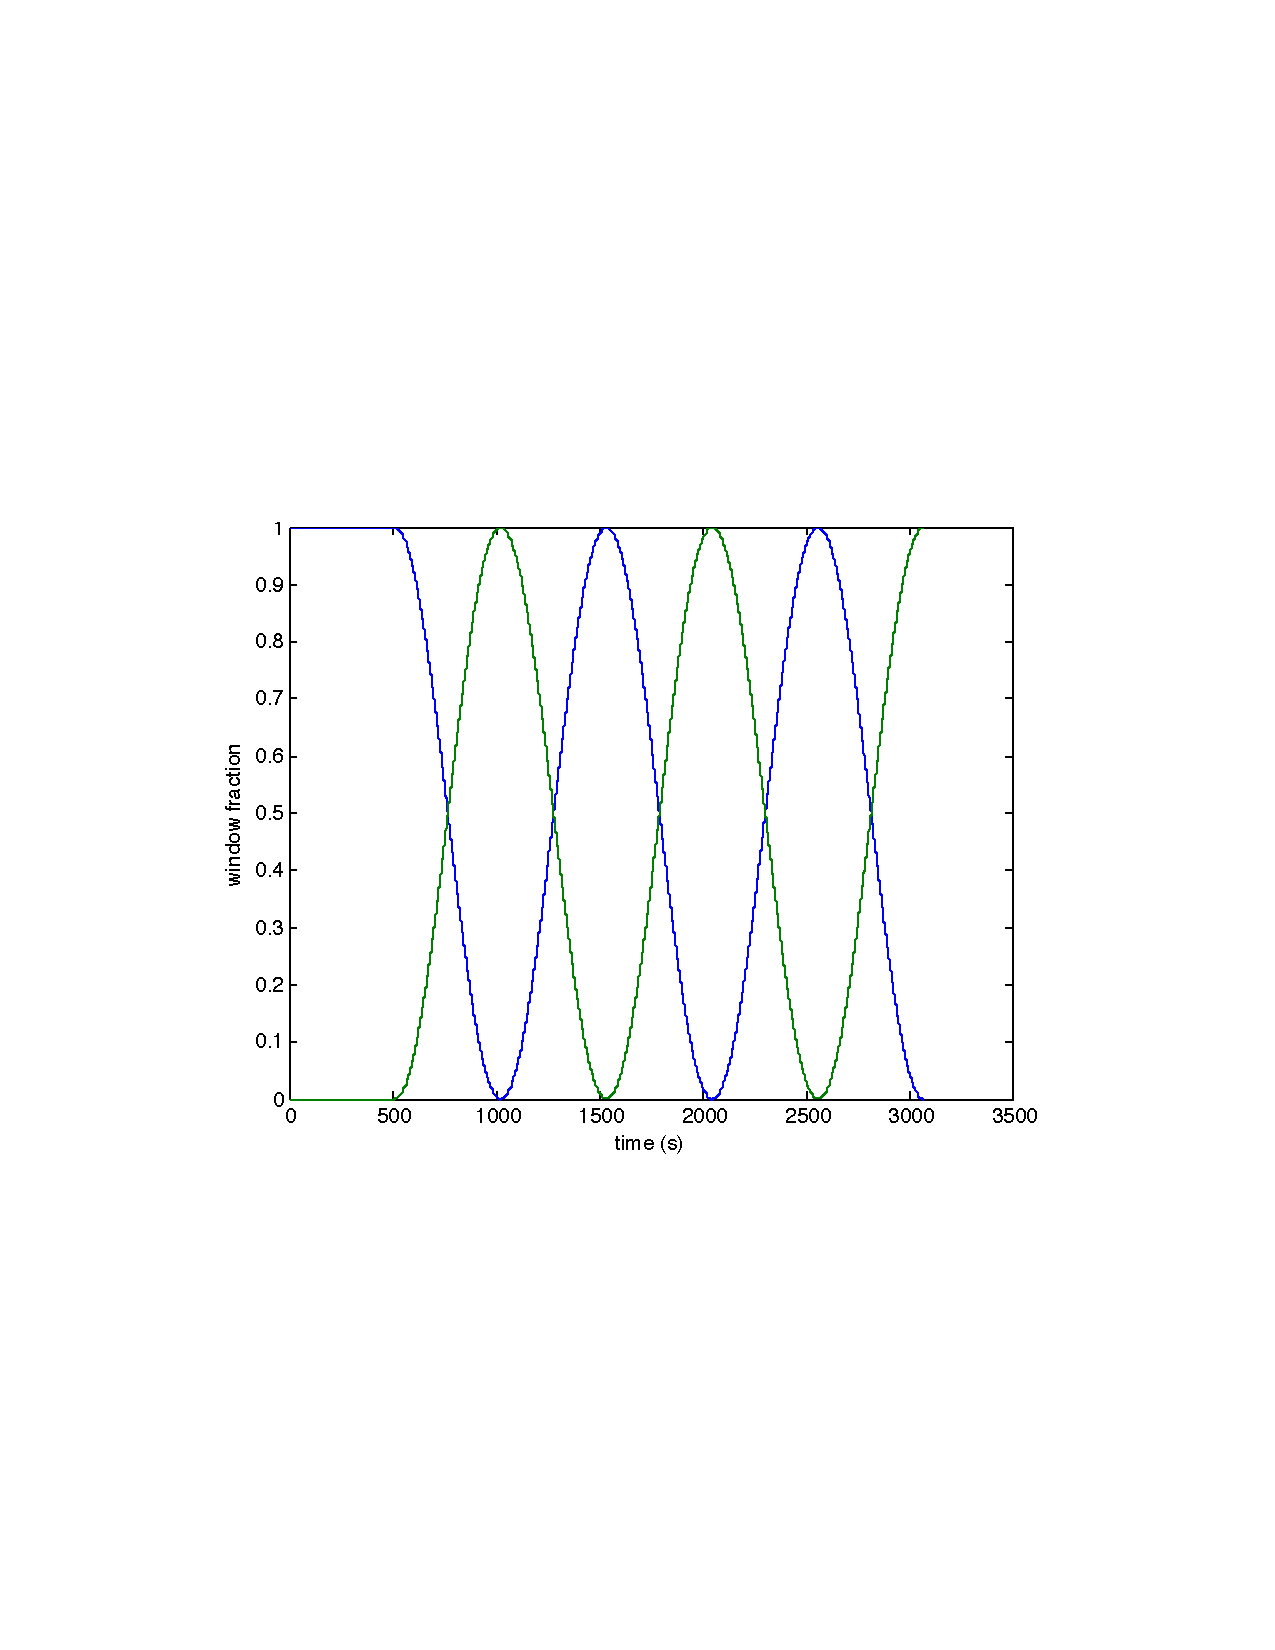
\includegraphics[width=0.85\paperwidth,height=0.5\paperheight]{plots/hann-windows}}


\emph{Windowing}

One job per science segment, filters calculated for 1024 s windows

50\%-overlapping Hann windows smoothly join filters $g_{A,B}$ and$h(t)$

$h(t)=\hat{s}(t)-\frac{1}{2}\left(g_{A}\left[1+\cos\frac{2\pi t}{1024\textup{\textup{{s}}}}\right]+g_{B}\left[1-\cos\frac{2\pi t}{1024\textup{{s}}}\right]\right)\times N(t)$

\url{matapps/packages/detchar/AMPS/trunk/eleutheria.m}
\end{figure}

\end{onlyenv}%{}



\lyxframeend{}\subsection*{Transfer function filters}
\lyxframeend{}\lyxframe{Transfer function filters}

\begin{onlyenv}%{}
<1>

\begin{figure}
\caption{\protect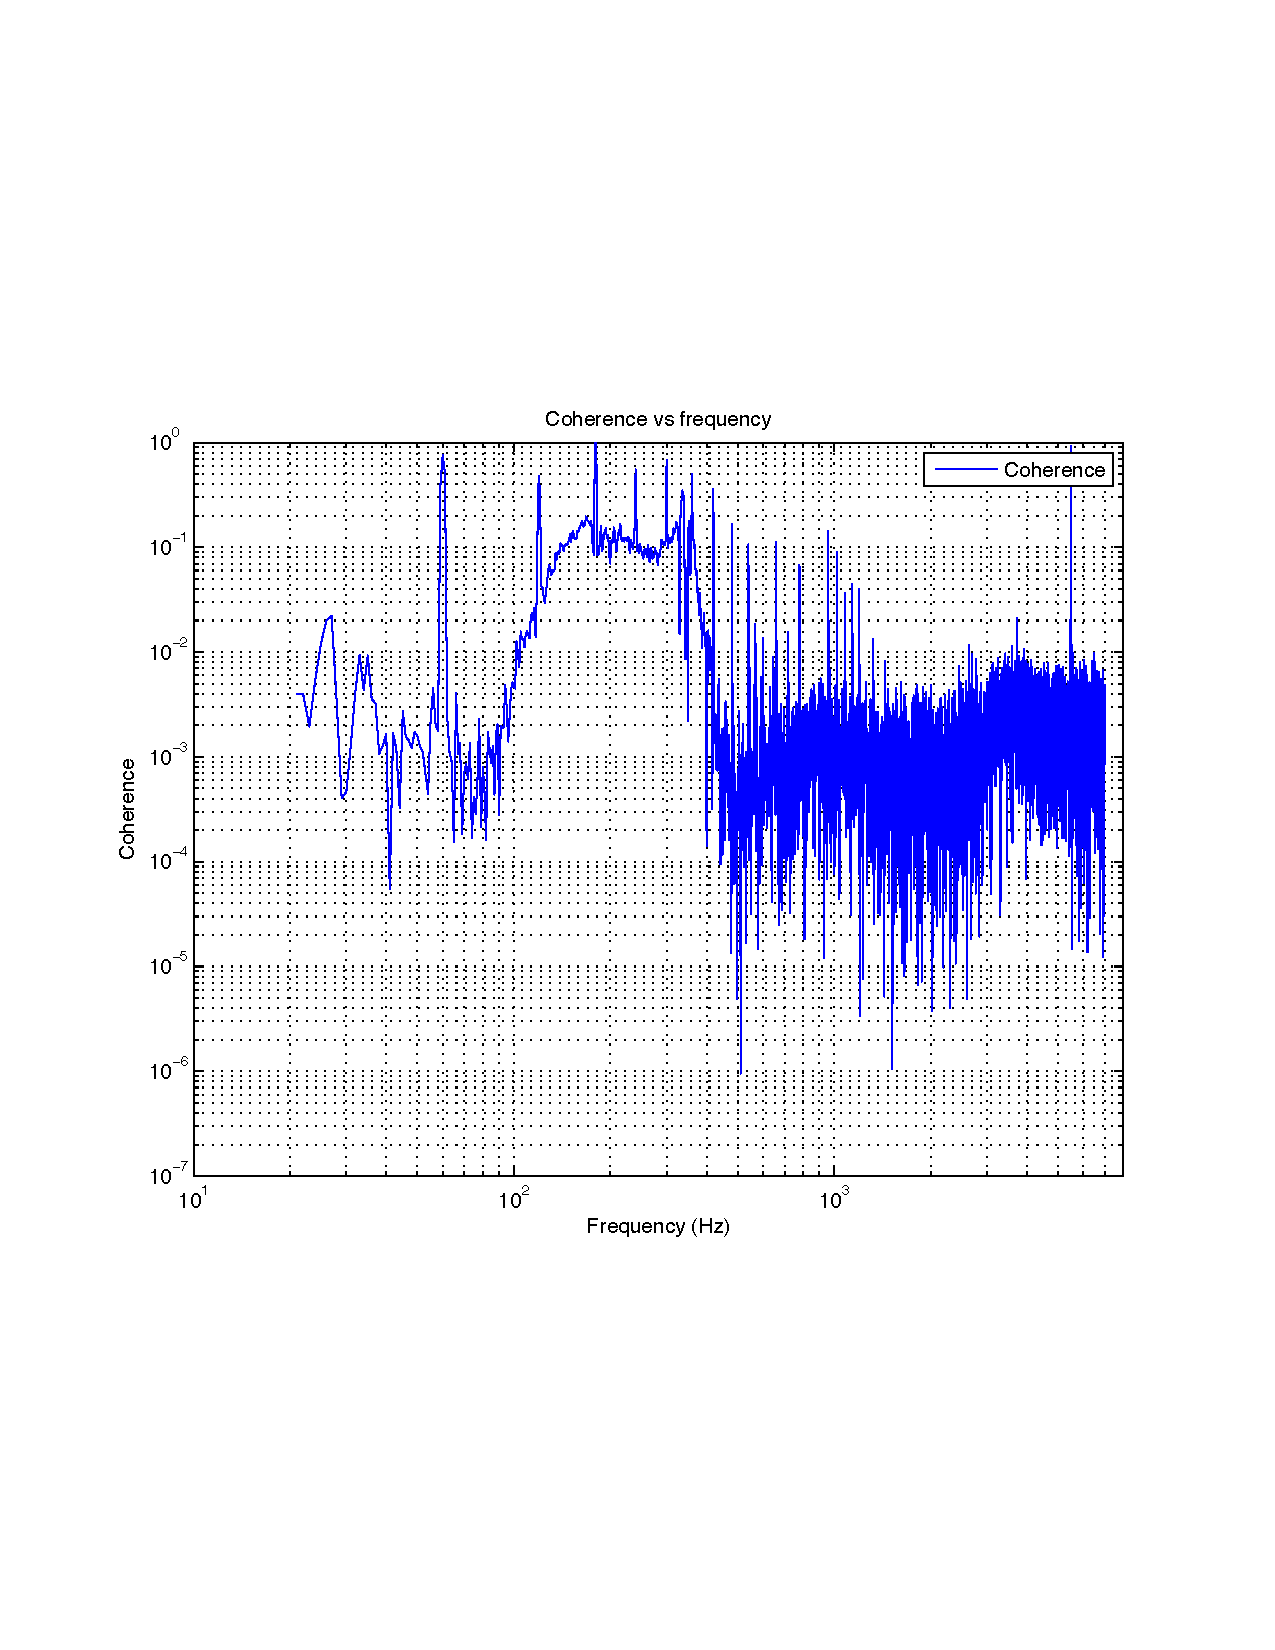
\includegraphics[width=0.45\paperwidth,height=0.55\paperheight]{plots/clip-MICH-coh}\protect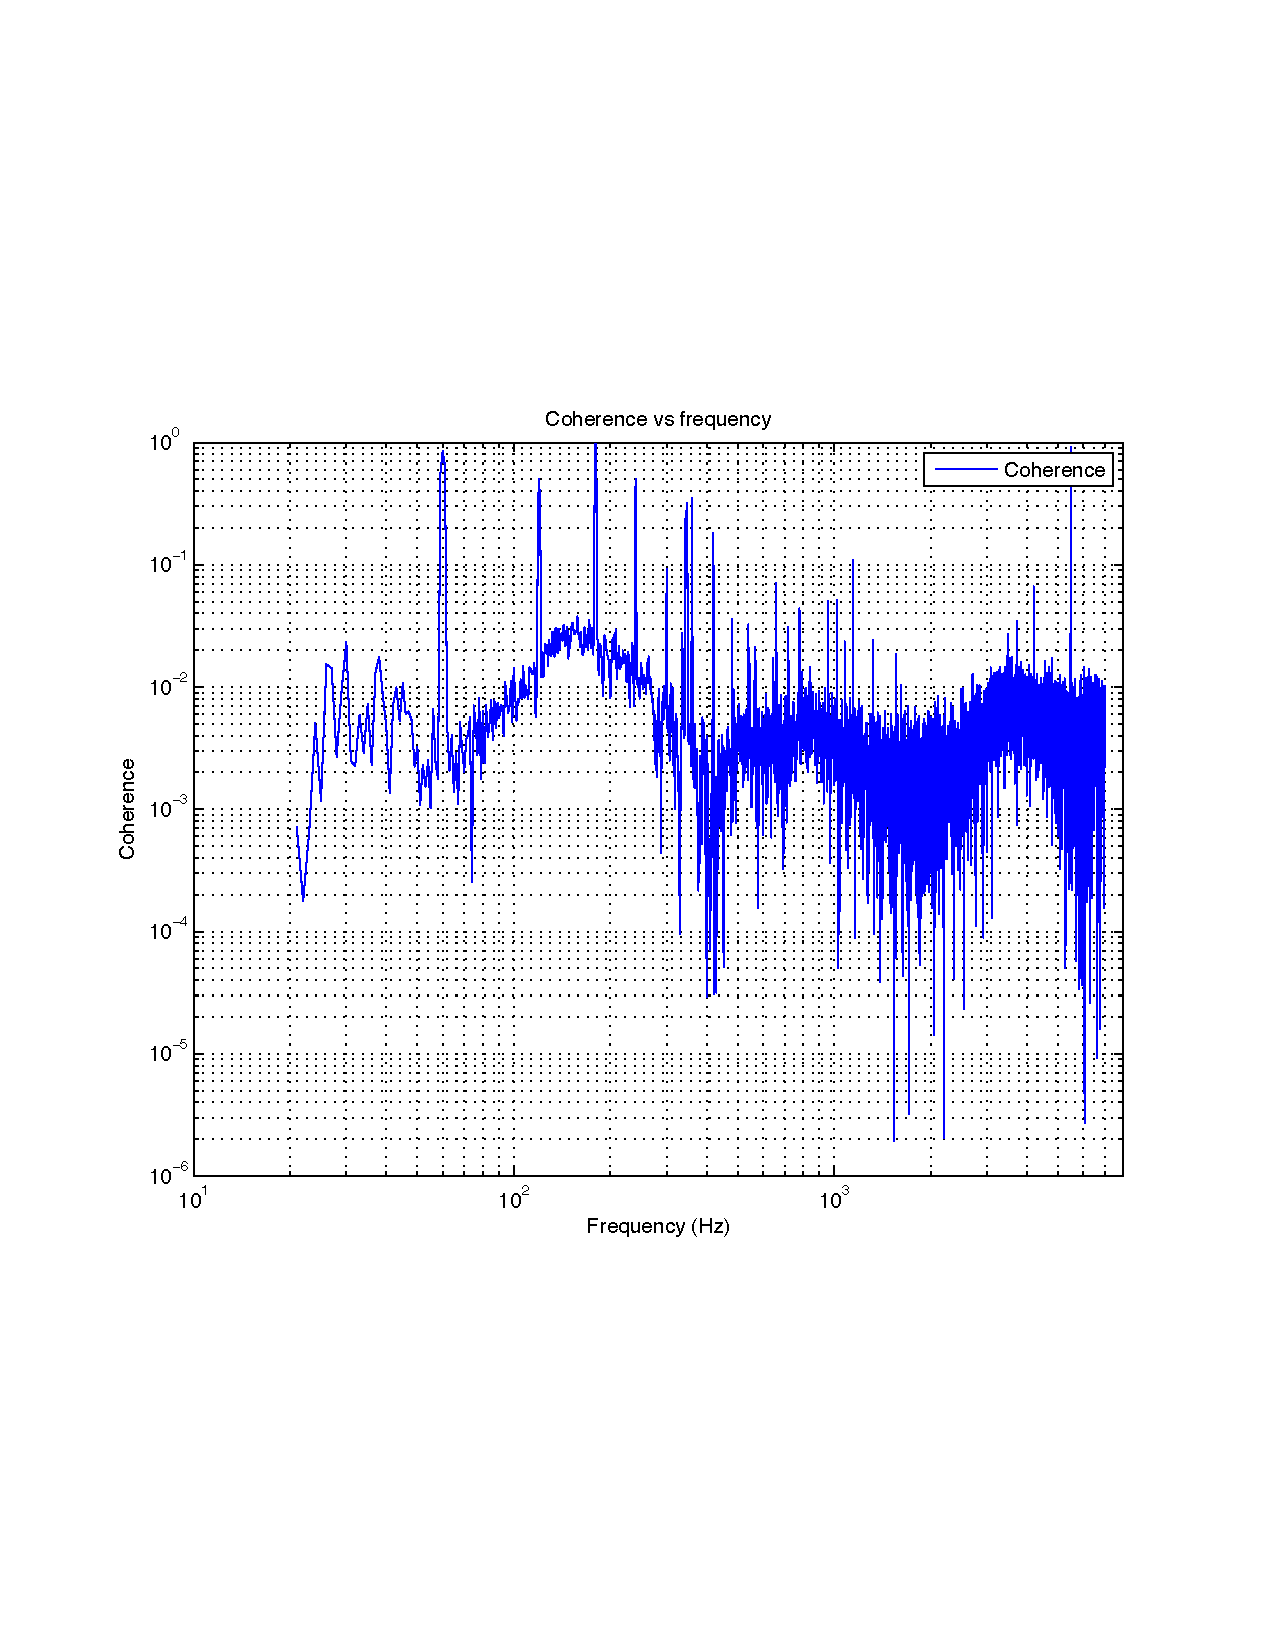
\includegraphics[width=0.45\paperwidth,height=0.55\paperheight]{plots/clip-PRC-coh}}


Coherence between h(t) and

MICH (left), PRC (right):

statistically-significant coherence justifies TF fit

(sample: 2010-03-21T0000Z)
\end{figure}

\end{onlyenv}%{}

\begin{onlyenv}%{}
<2>

\begin{figure}
\caption{\protect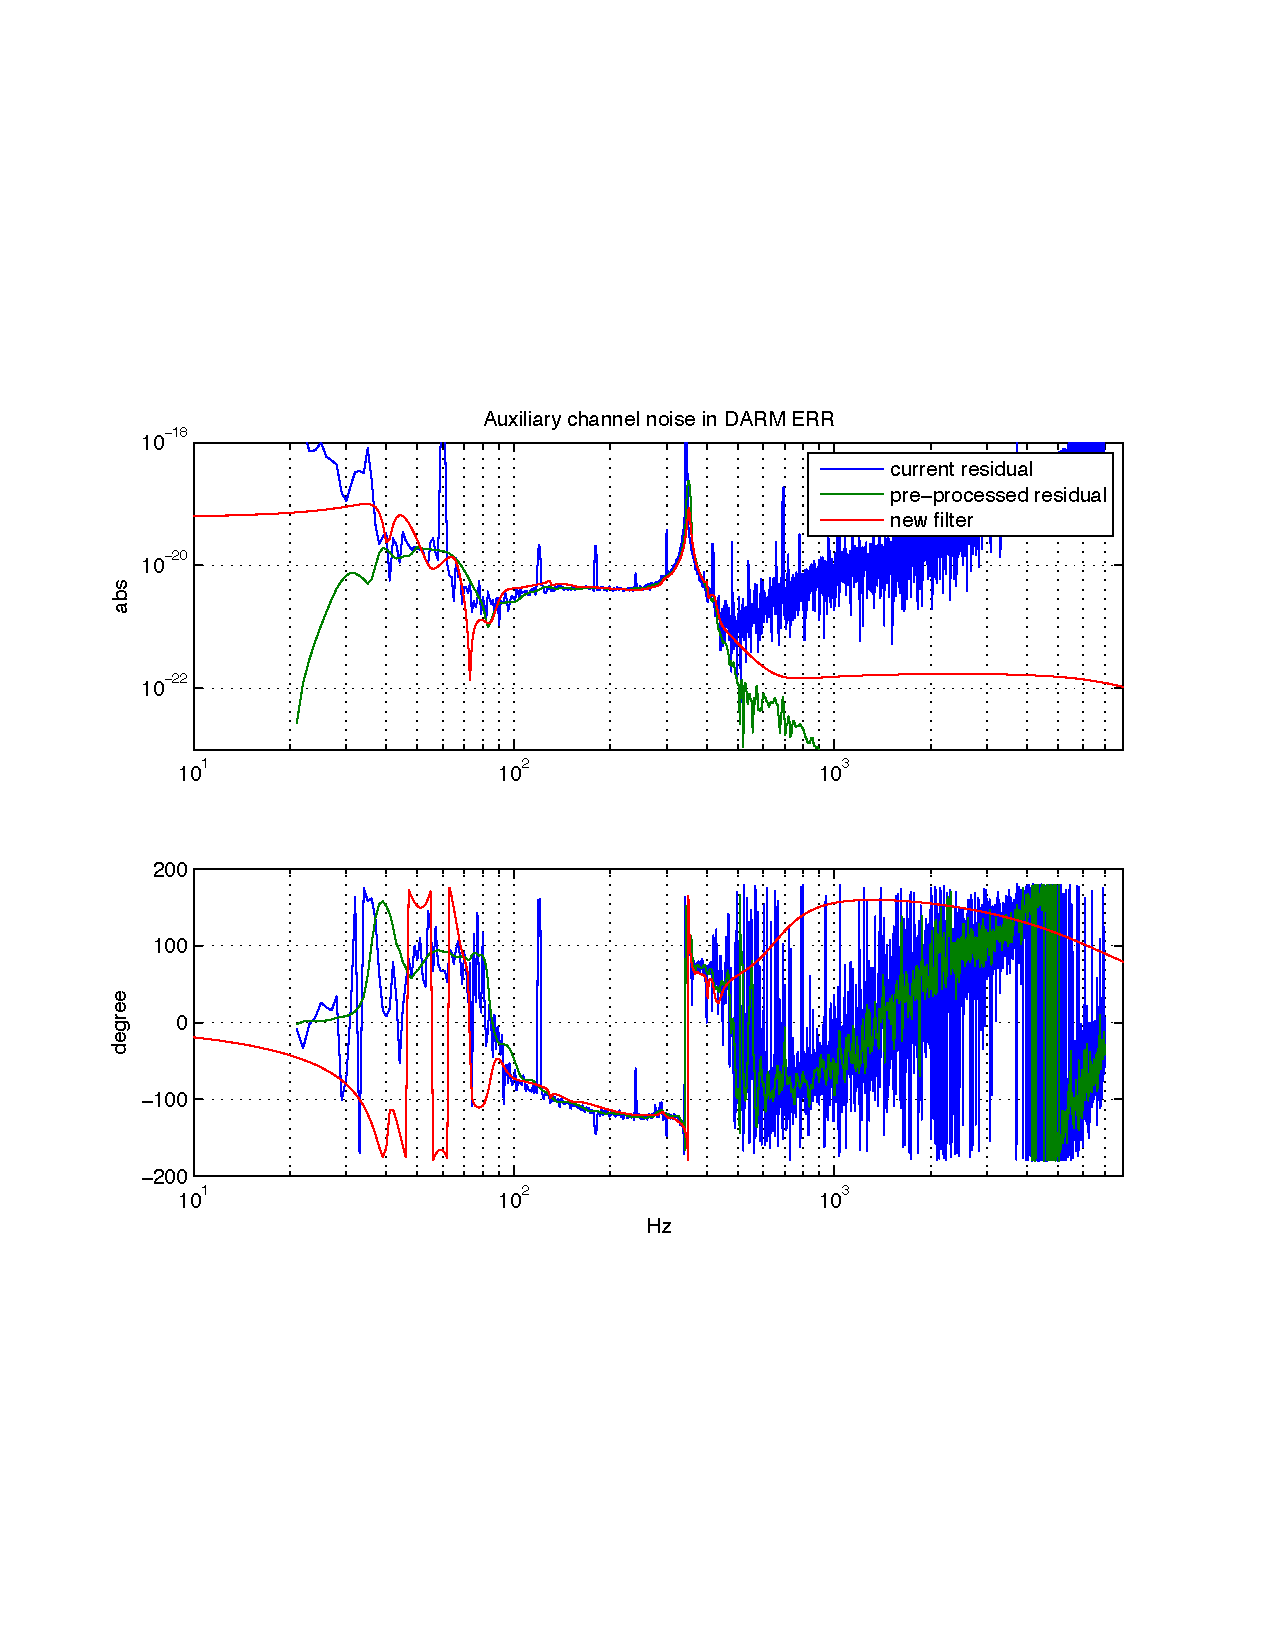
\includegraphics[width=0.45\paperwidth,height=0.55\paperheight]{plots/clip-MICH-fit}\protect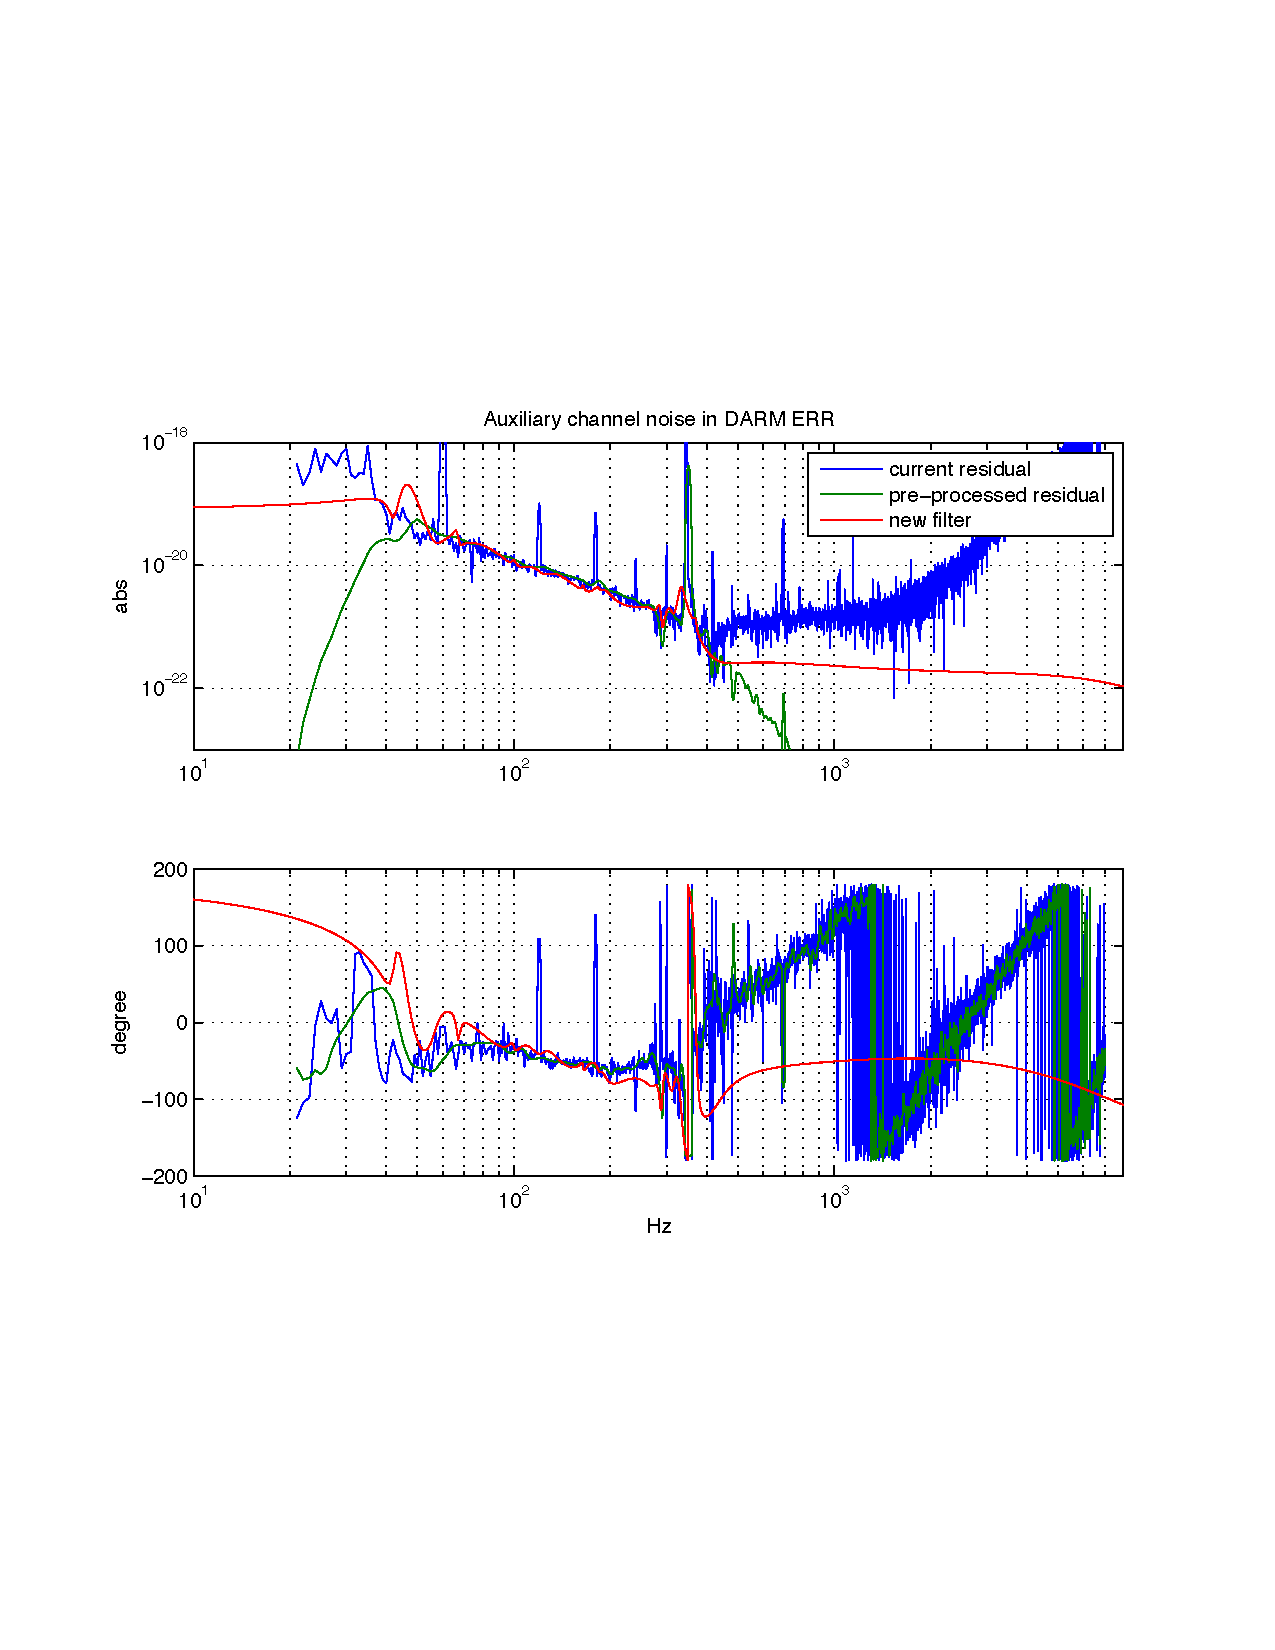
\includegraphics[width=0.45\paperwidth,height=0.55\paperheight]{plots/clip-PRC-fit}}


Transfer function (TF) fit for h(t) with

MICH (left), PRC (right):

TF smoothed before fitting to coherent band using Vectfit

(sample: 2010-03-21T0000Z)
\end{figure}

\end{onlyenv}%{}

\begin{onlyenv}%{}
<3>

\begin{figure}


\caption{\protect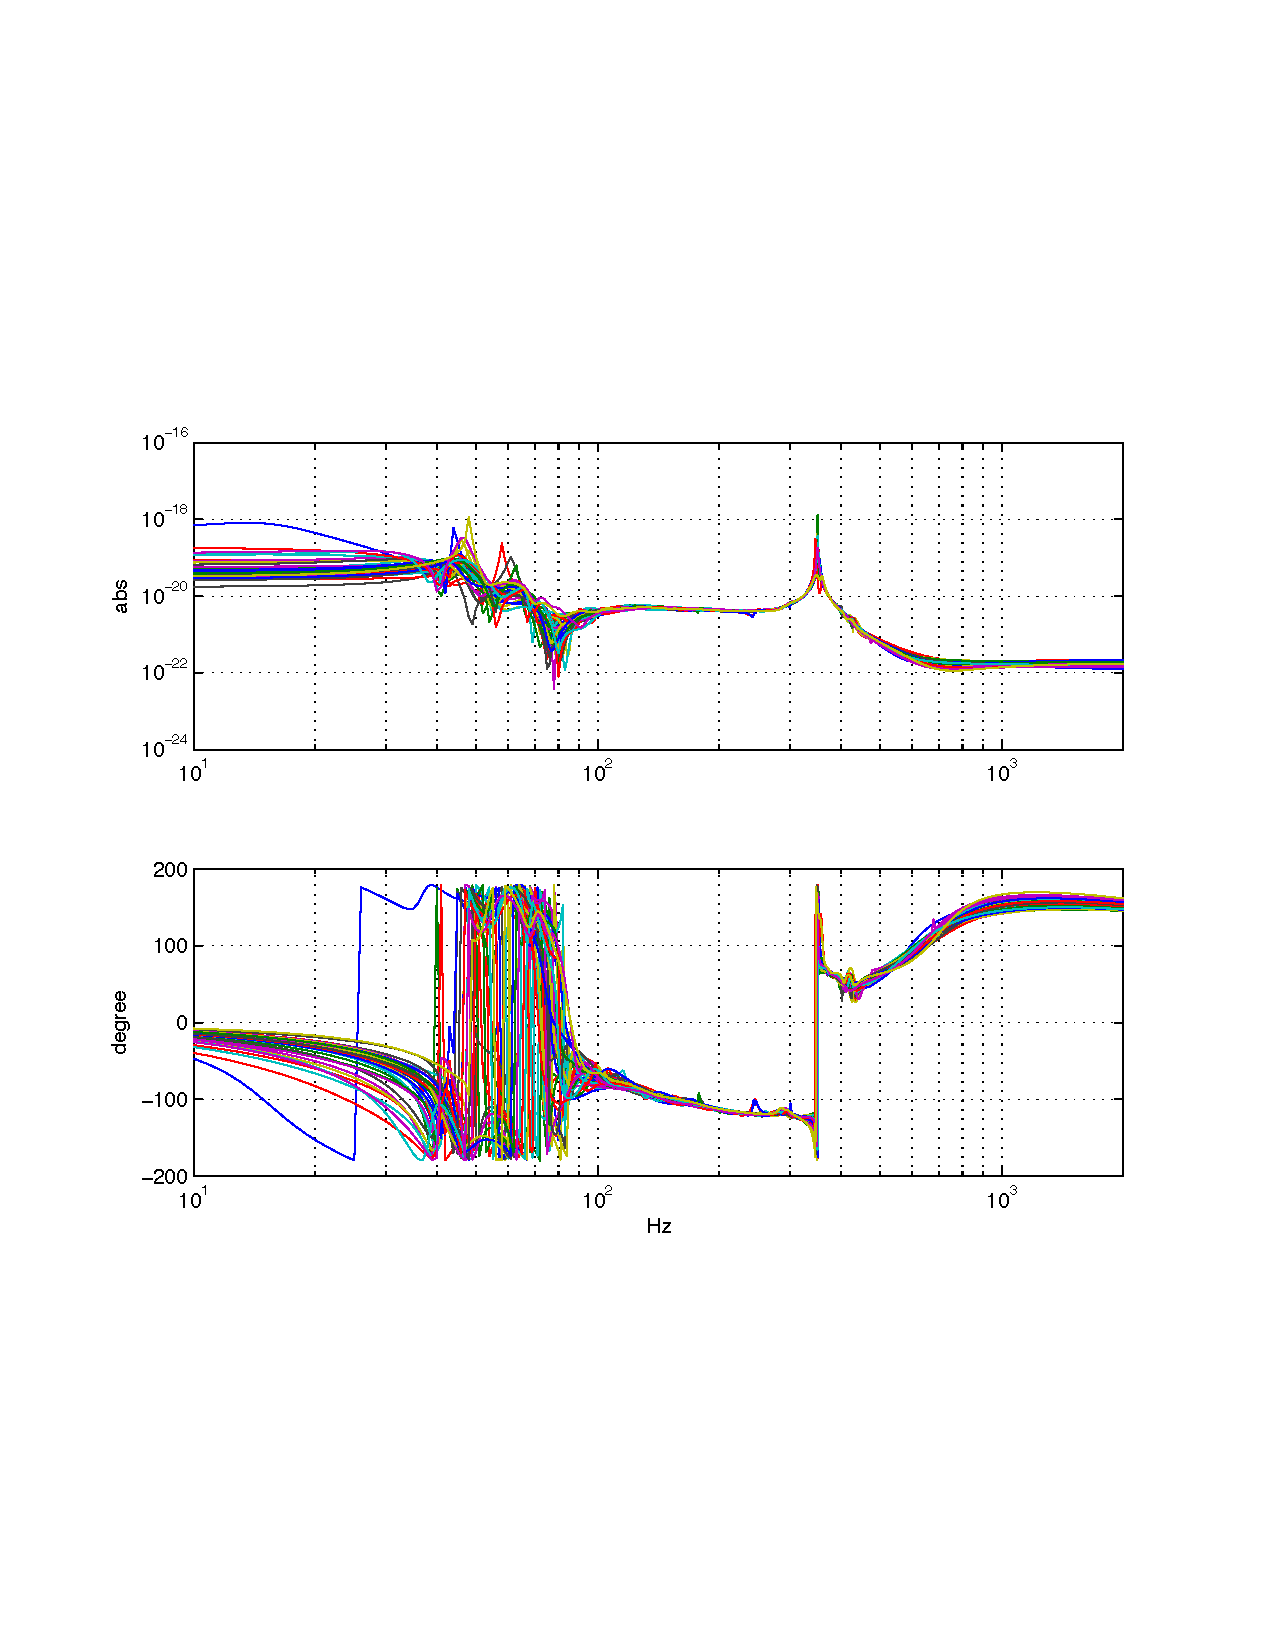
\includegraphics[width=0.45\paperwidth,height=0.55\paperheight]{plots/clip-MICH-many}\protect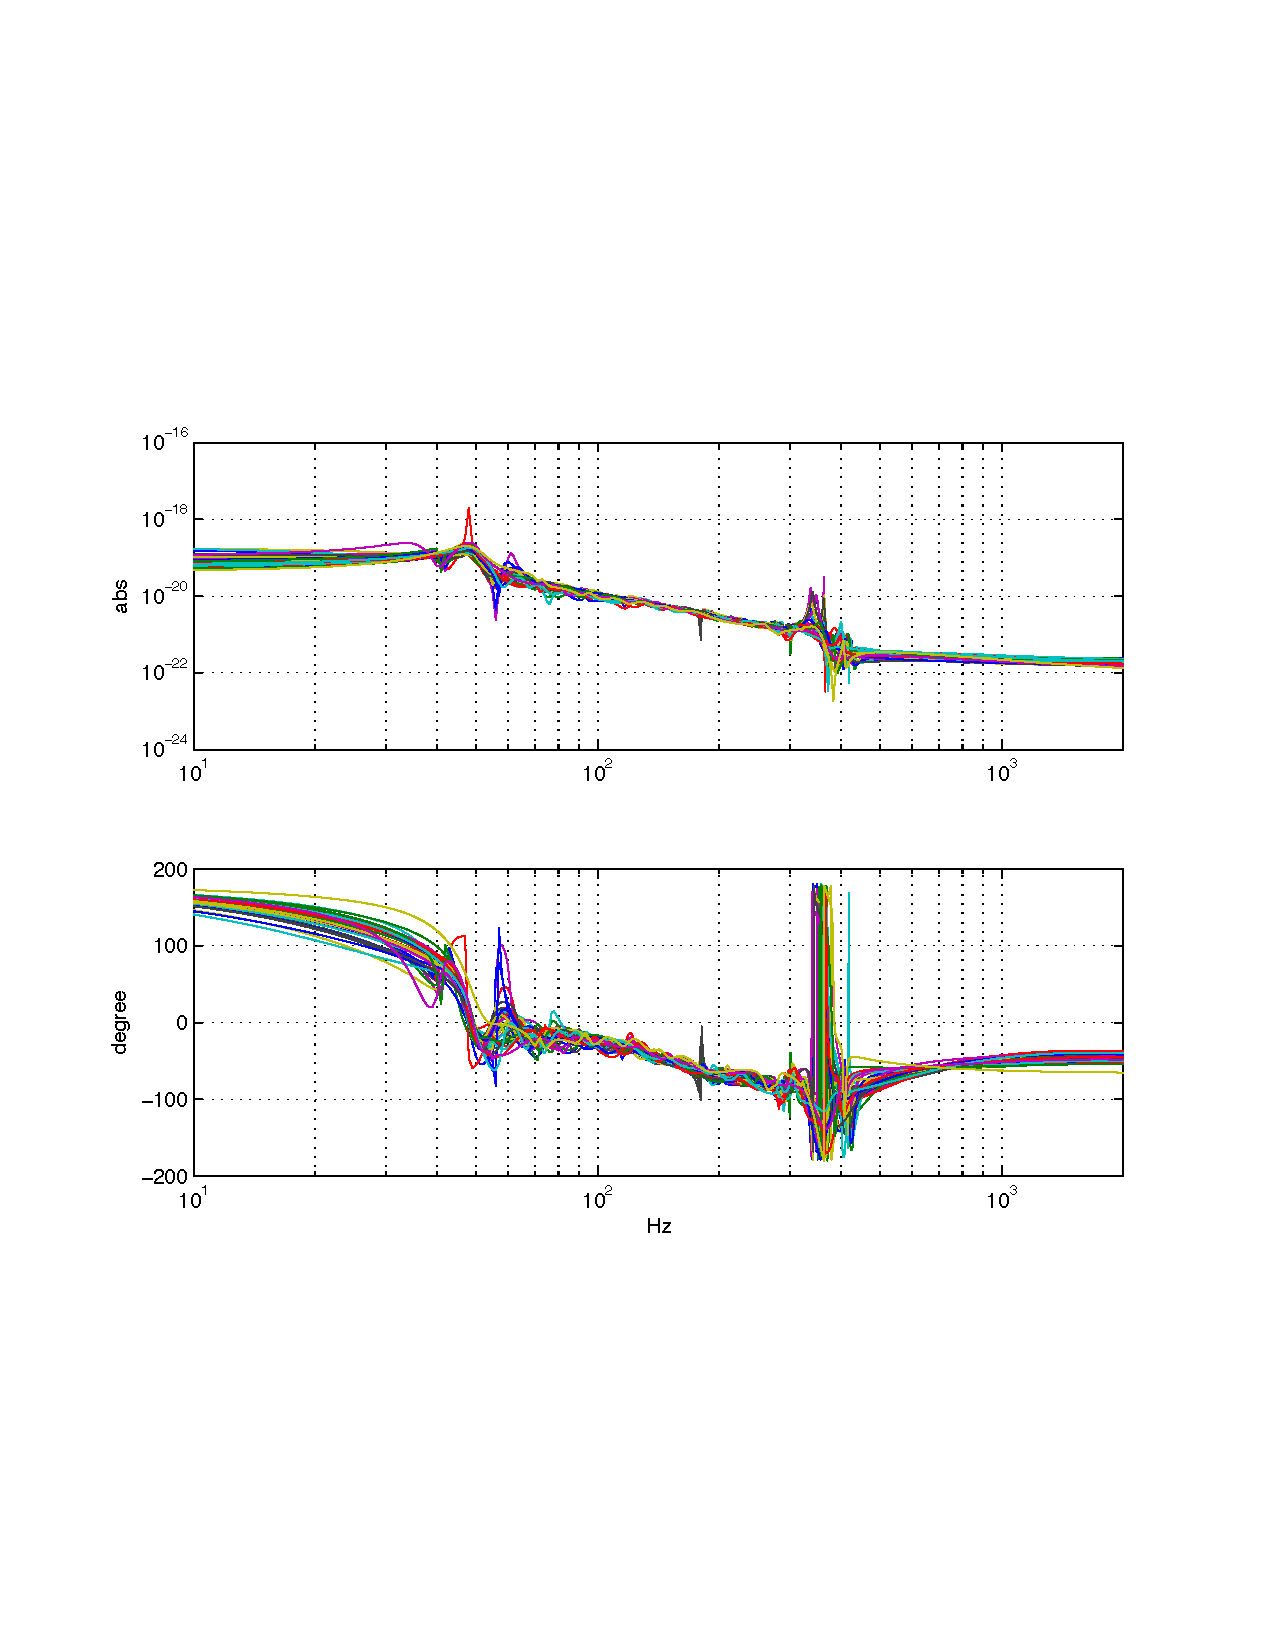
\includegraphics[width=0.45\paperwidth,height=0.55\paperheight]{plots/clip-PRC-many}}


Variation in TF fits over science segment

Each color is one 1024 s window

MICH (left), PRC (right)

(sample: 2010-03-20T2316Z/2010-03-21T0407Z)
\end{figure}

\end{onlyenv}%{}

\begin{onlyenv}%{}
<4>

\begin{figure}


\caption{\protect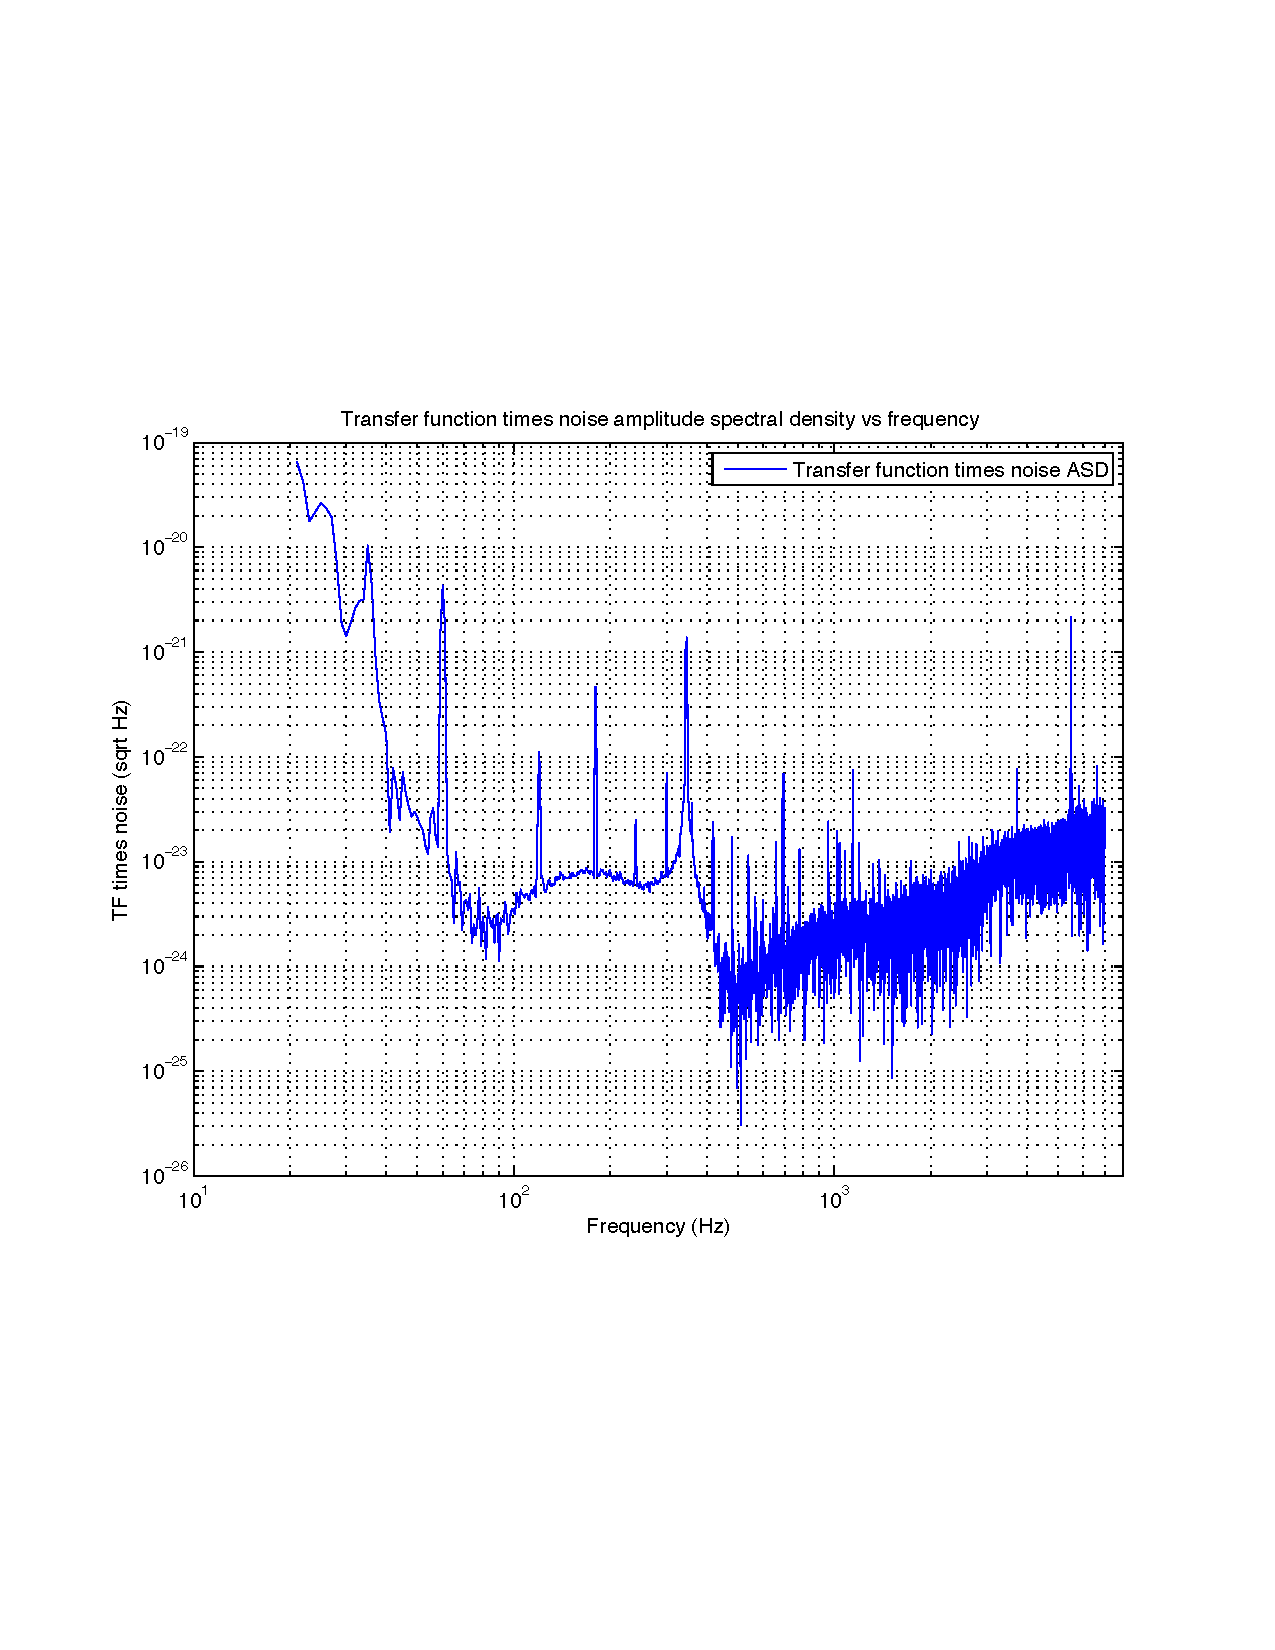
\includegraphics[width=0.45\paperwidth,height=0.55\paperheight]{plots/clip-MICH-sub}\protect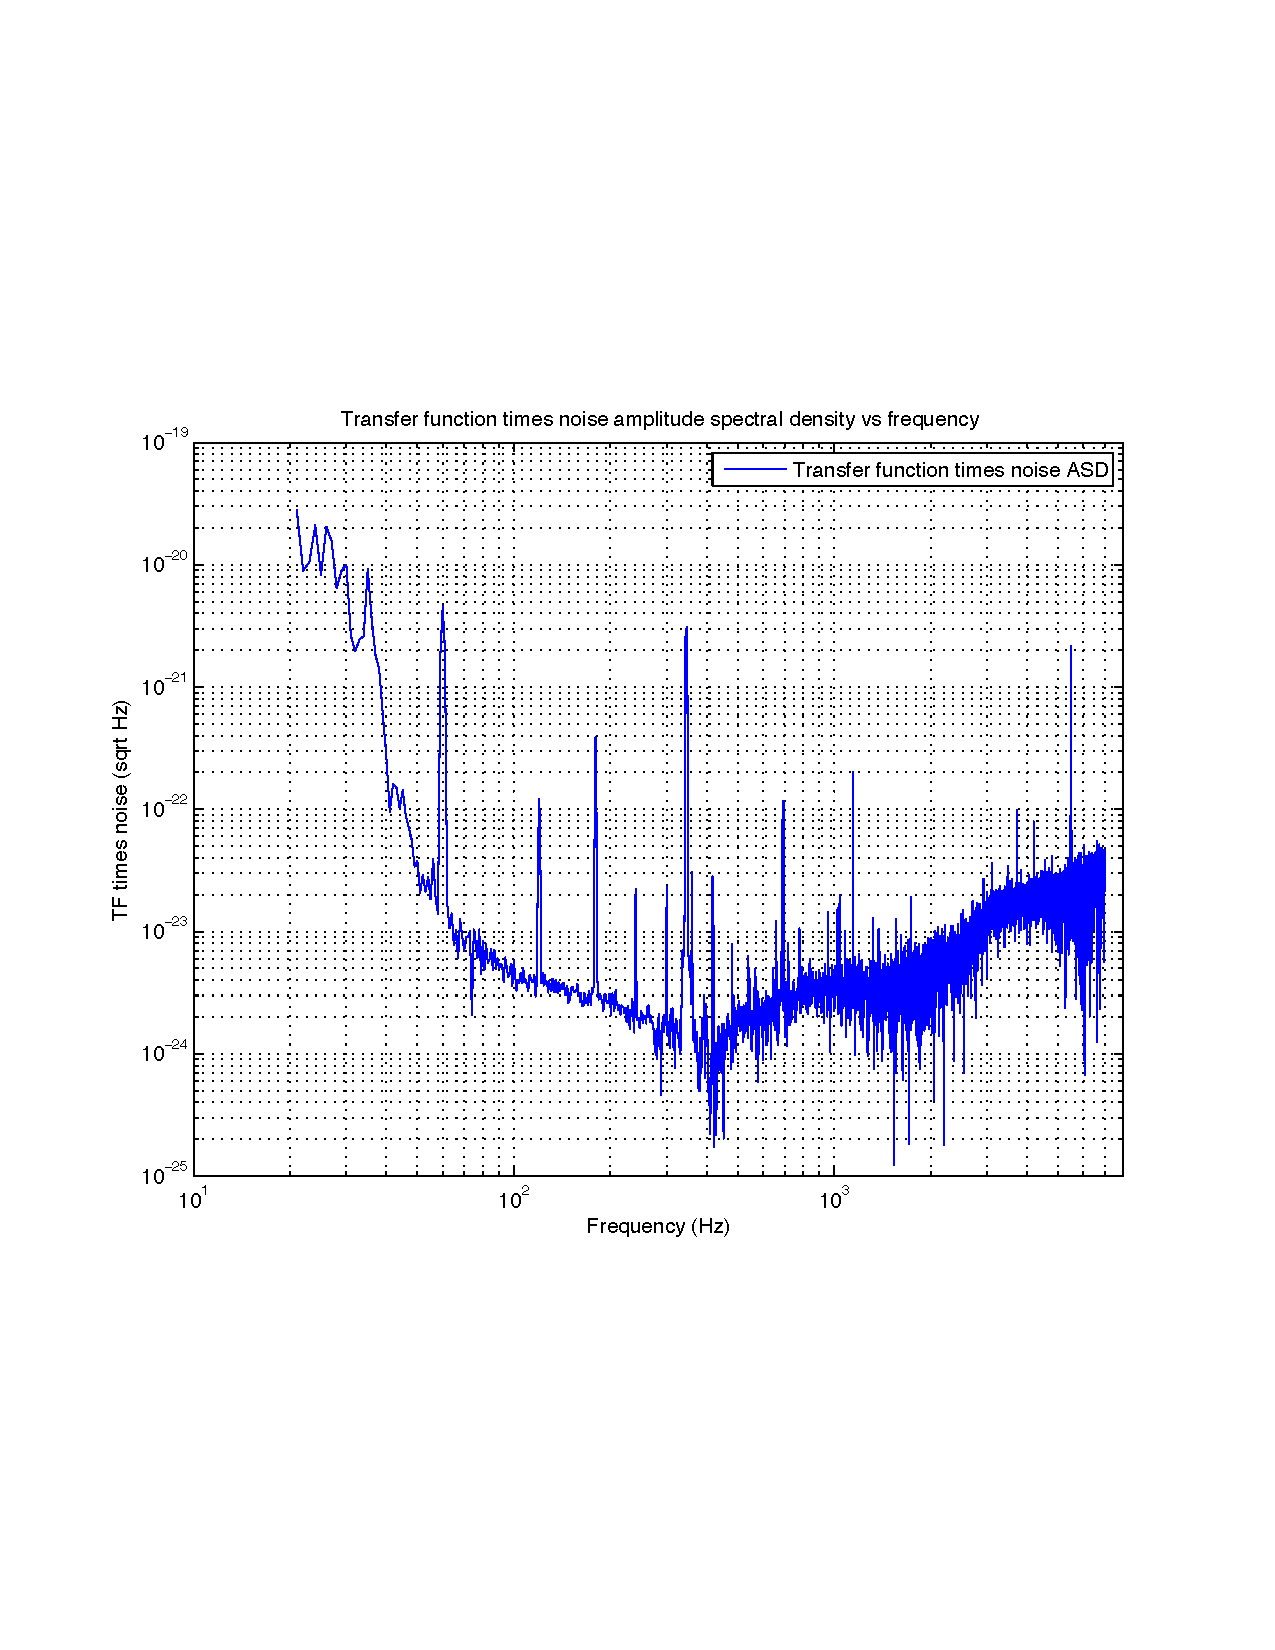
\includegraphics[width=0.45\paperwidth,height=0.55\paperheight]{plots/clip-PRC-sub}}


Estimated subtraction in amplitude spectral density (ASD)

(equal to TF times noise)

MICH (left), PRC (right)

(sample: 2010-03-21T0000Z)
\end{figure}

\end{onlyenv}%{}



\lyxframeend{}\section{Frequency-fit, time-applied feedforward filtering}


\lyxframeend{}\subsection*{Amplitude spectral density comparisons}


\lyxframeend{}\lyxframe{Amplitude spectral density comparisons}


\note[item]{Show both graphs! Explain the process of generating a servo using
each method.}
\begin{onlyenv}%{}
<1>

\begin{figure}
\caption{\protect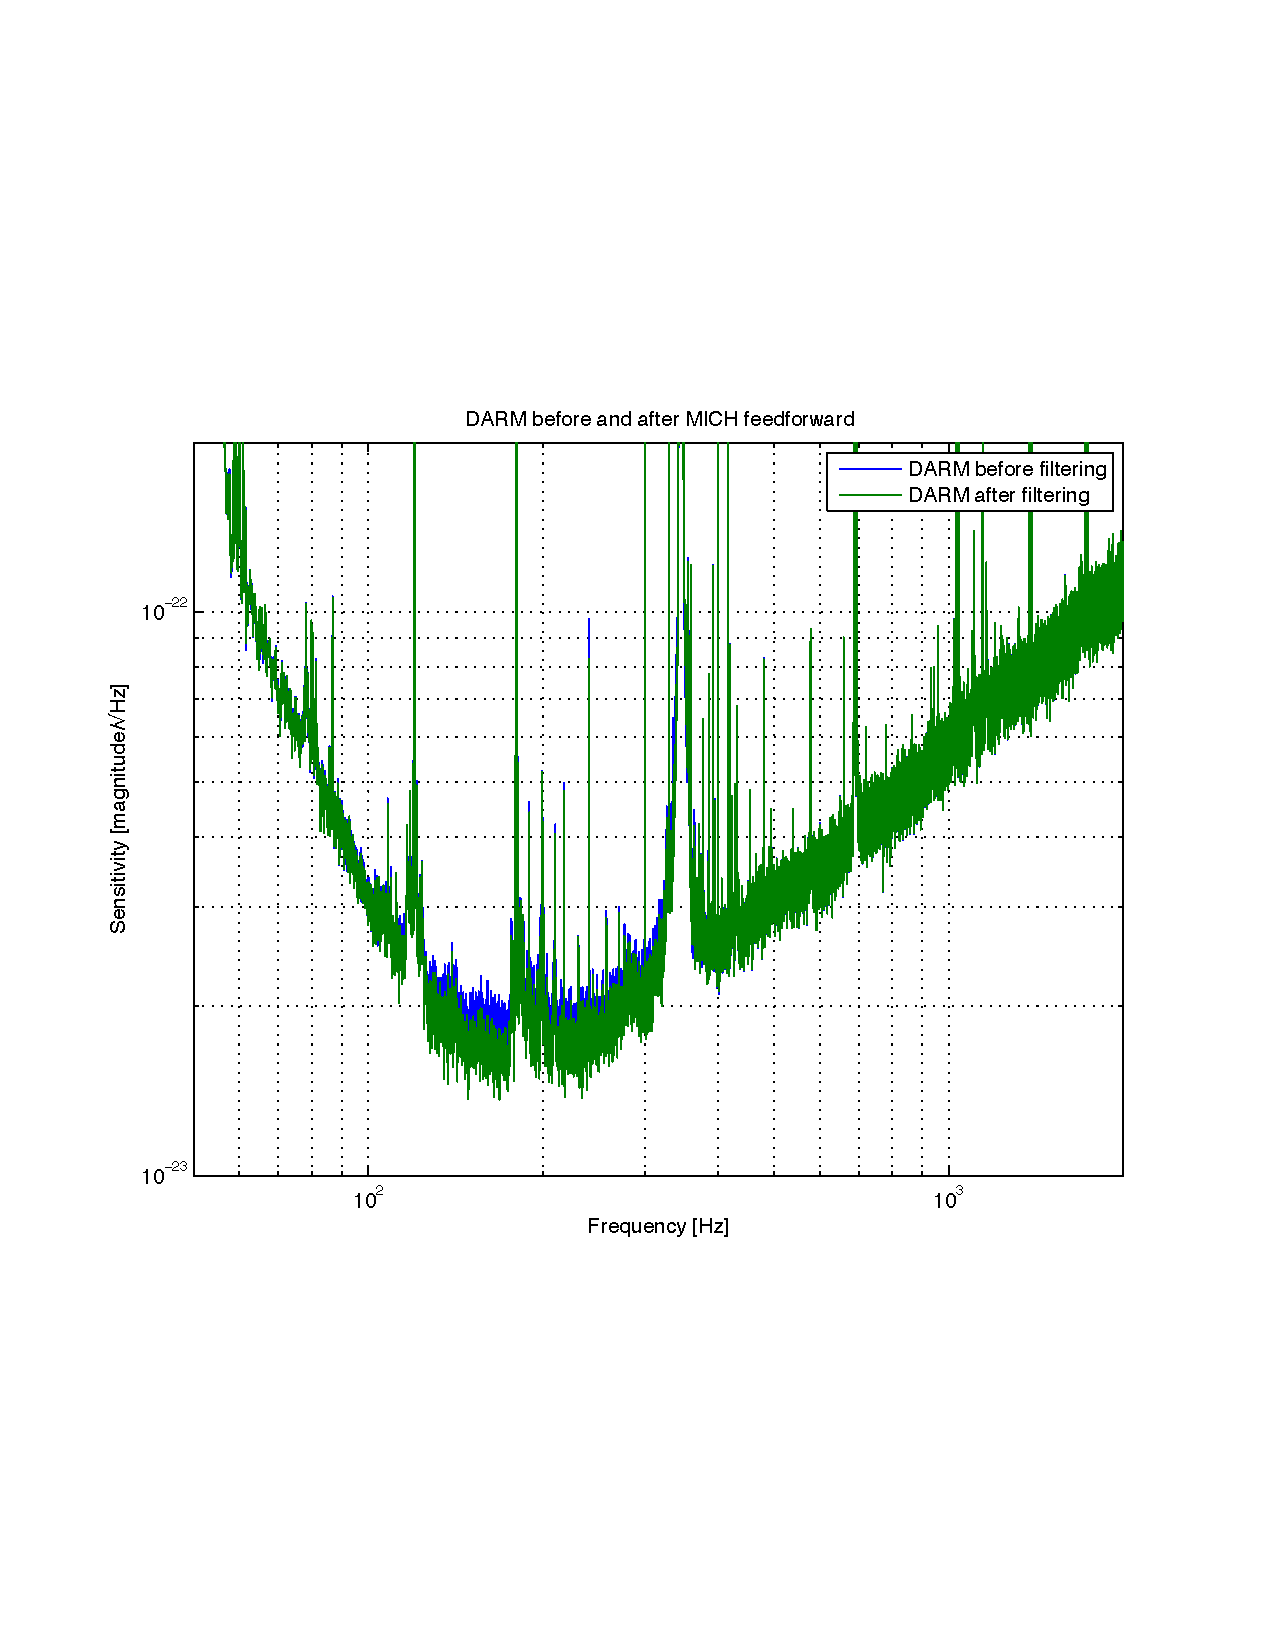
\includegraphics[height=0.6\paperheight]{plots/clip-exemplar-ASD}}


Exemplar H1 before-and-after ASD 

MICH \& PRC both filtered, +1.1 Mpc (5.9\%) inspiral range

(GPS 953164819 to 953165839, 2010-03-21)
\end{figure}

\end{onlyenv}%{}

\begin{onlyenv}%{}
<2>

\begin{figure}
\caption{\protect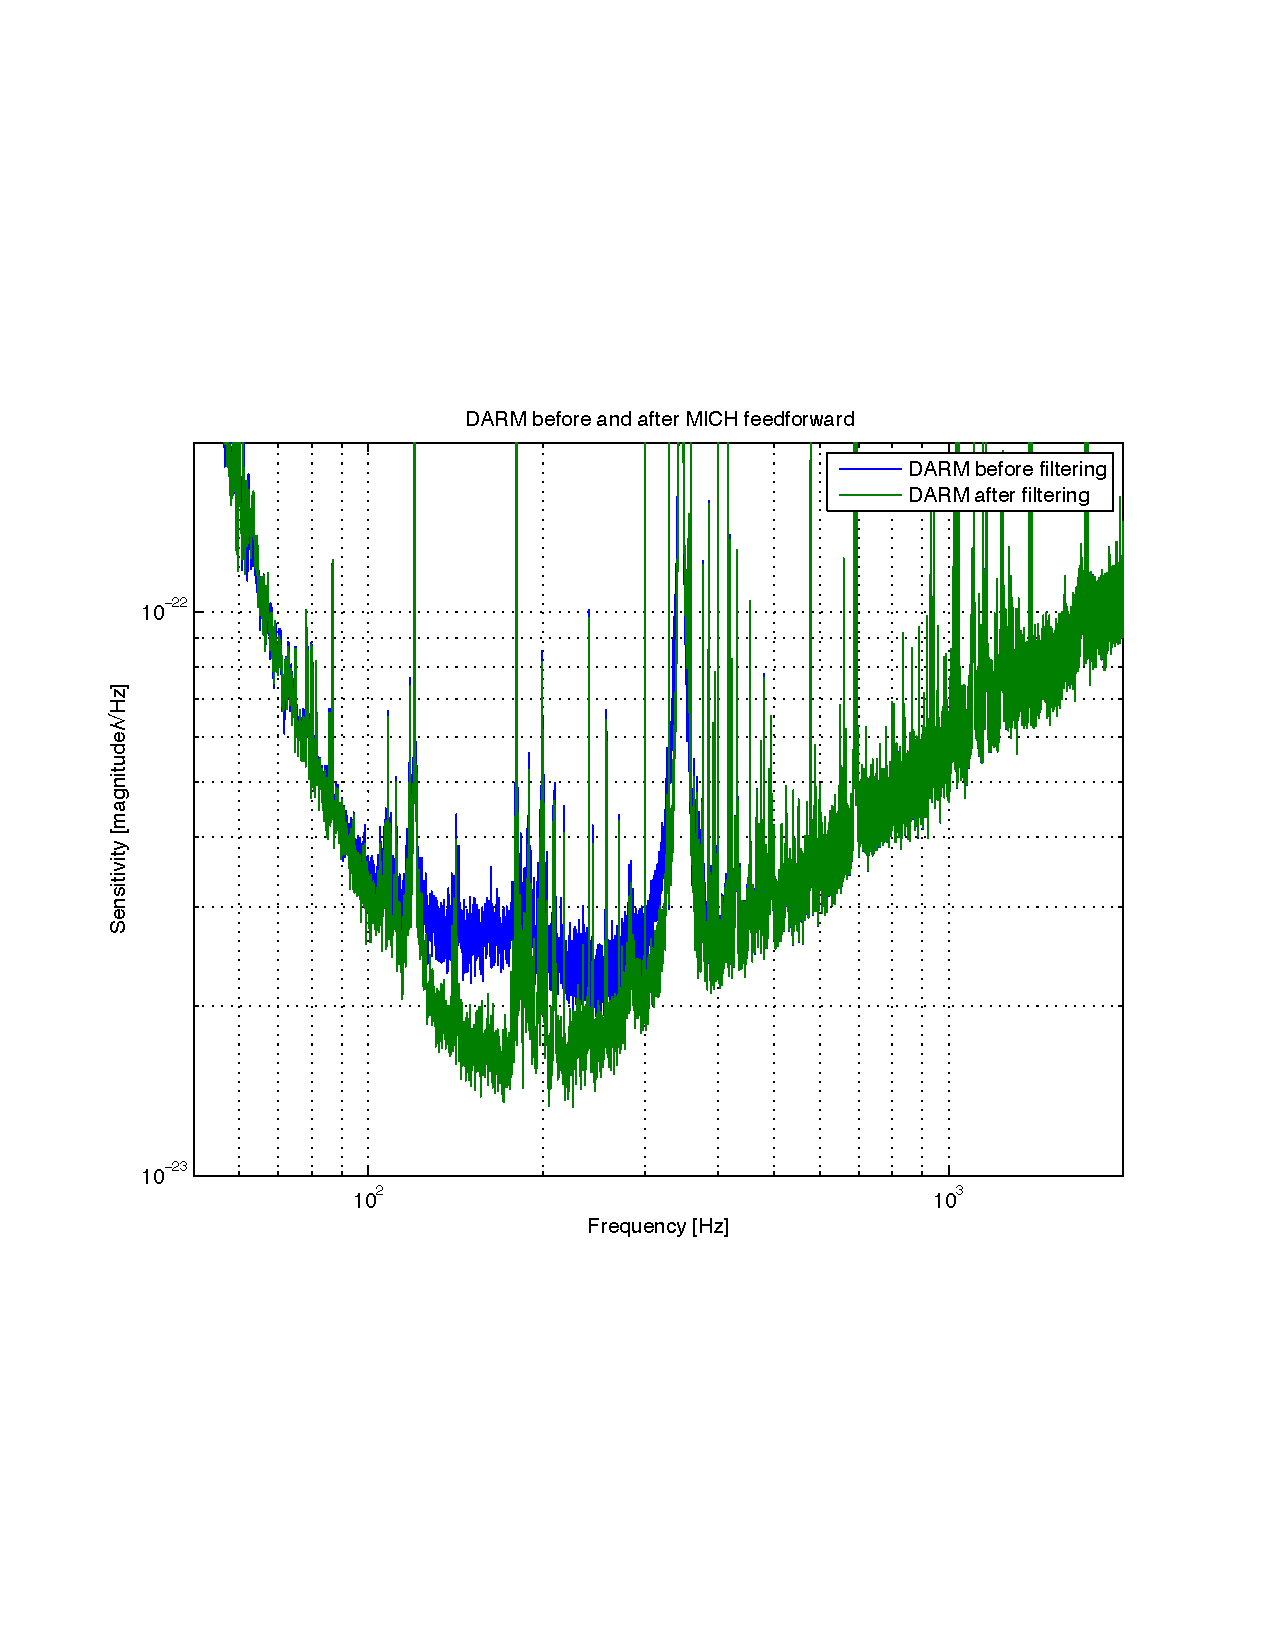
\includegraphics[height=0.6\paperheight]{plots/title_spectrum}}


Most dramatic H1 filtering

MICH \& PRC both filtered, +4.4 Mpc (29\%) inspiral range

(GPS 955187679 to 955188191, 2010-04-13)
\end{figure}

\end{onlyenv}%{}

\begin{onlyenv}%{}
<3>

\begin{figure}
\caption{\protect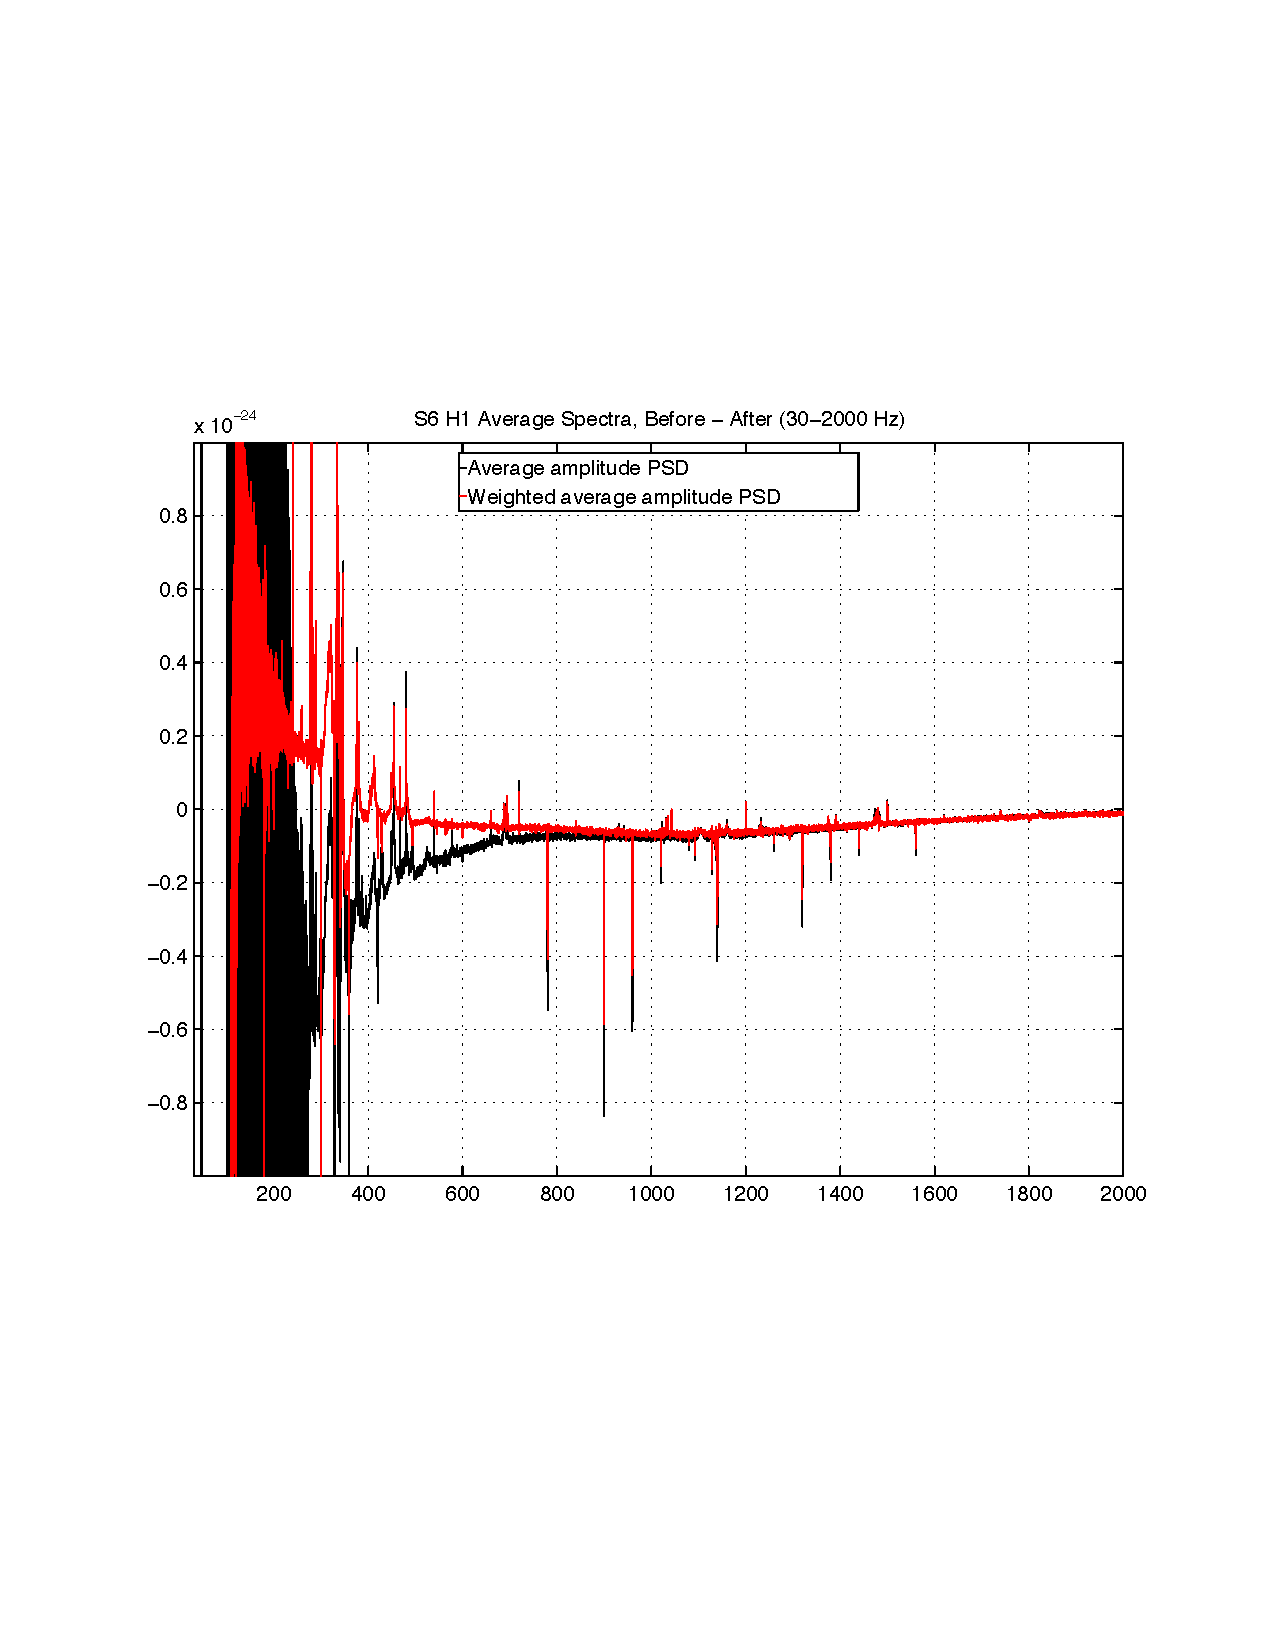
\includegraphics[width=0.4\paperwidth,height=0.65\paperheight]{plots/clip-diff}\protect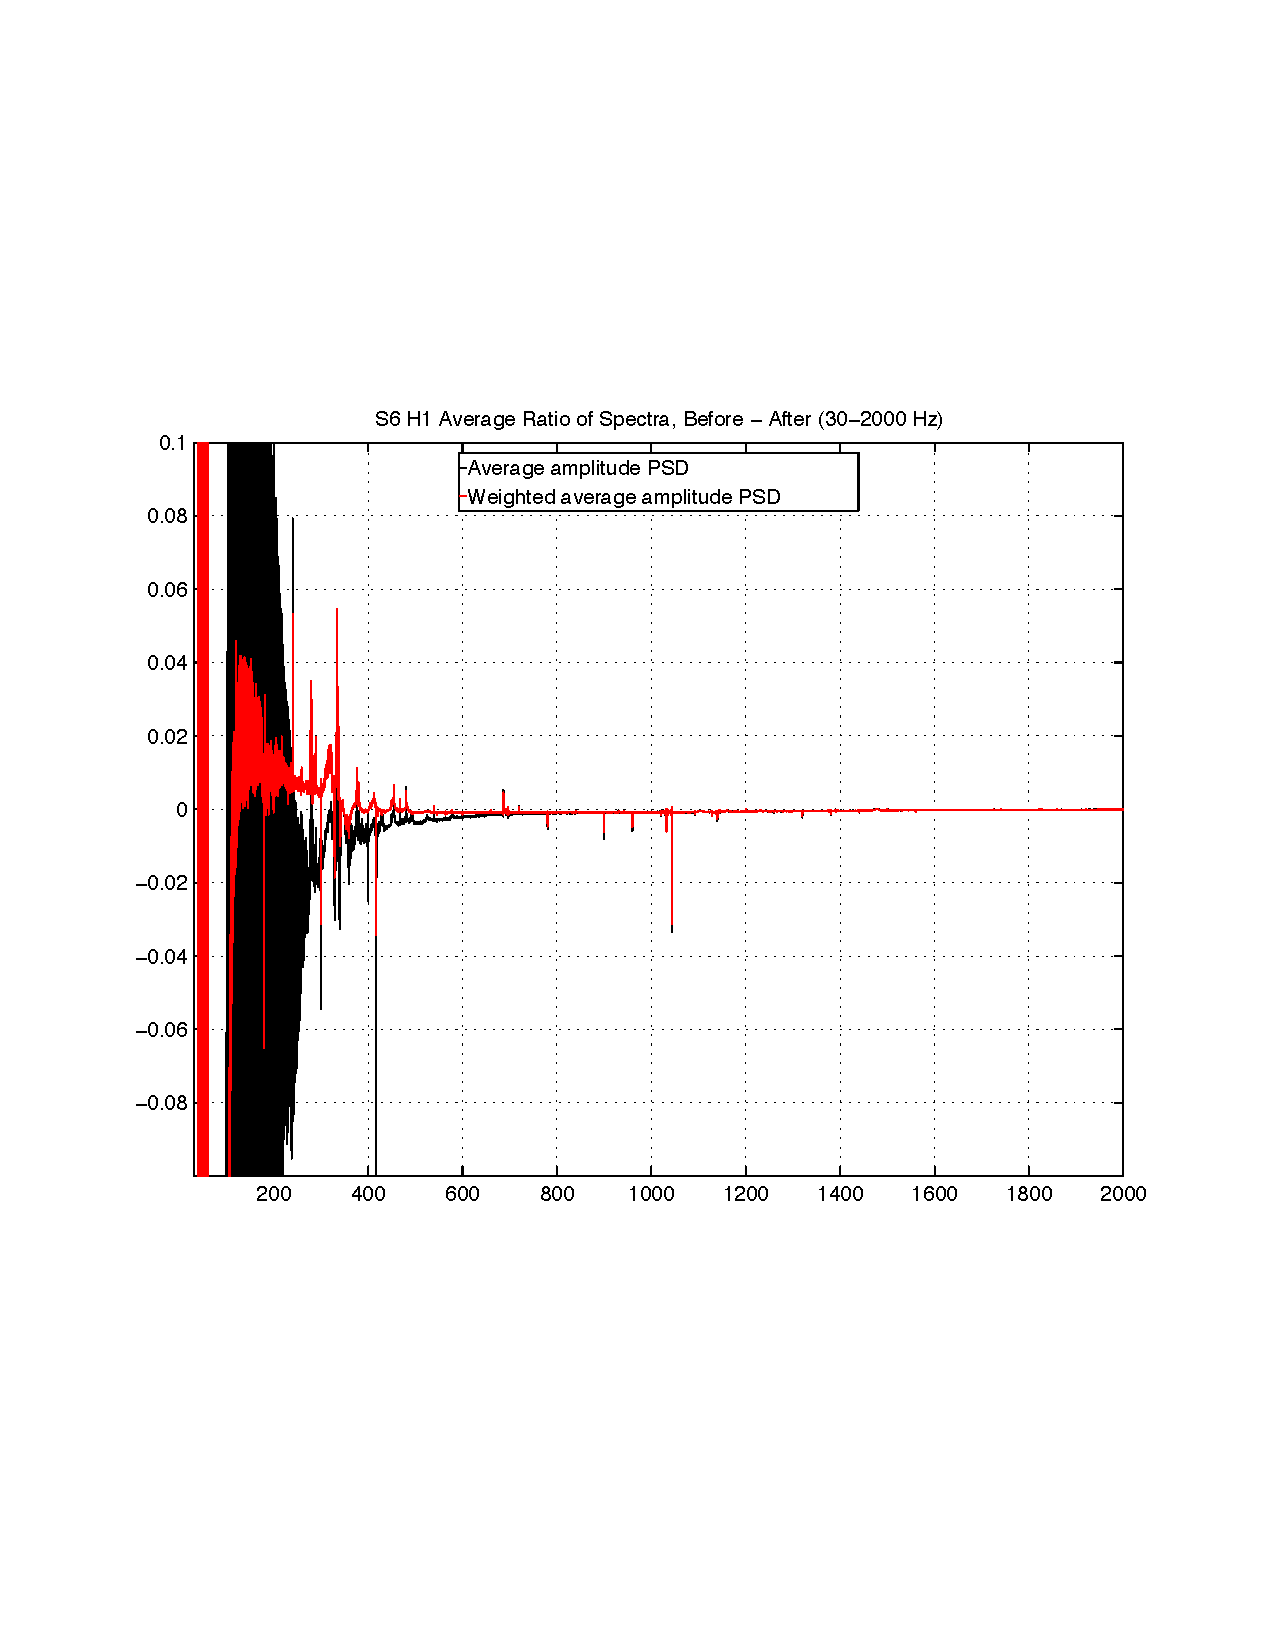
\includegraphics[width=0.4\paperwidth,height=0.65\paperheight]{plots/clip-diff-ratio}}


Left: \emph{(before - after); }Right: \emph{(before - after)/before}
\end{figure}


Arithmetic (black) and harmonic (red) mean ASD, 200 H1 jobs
\end{onlyenv}%{}

\lyxframeend{}\subsection*{S6 H1 and L1 results}


\lyxframeend{}\lyxframe{S6 H1 and L1 results}
\begin{onlyenv}%{}
<1>

\begin{figure}


\caption{\protect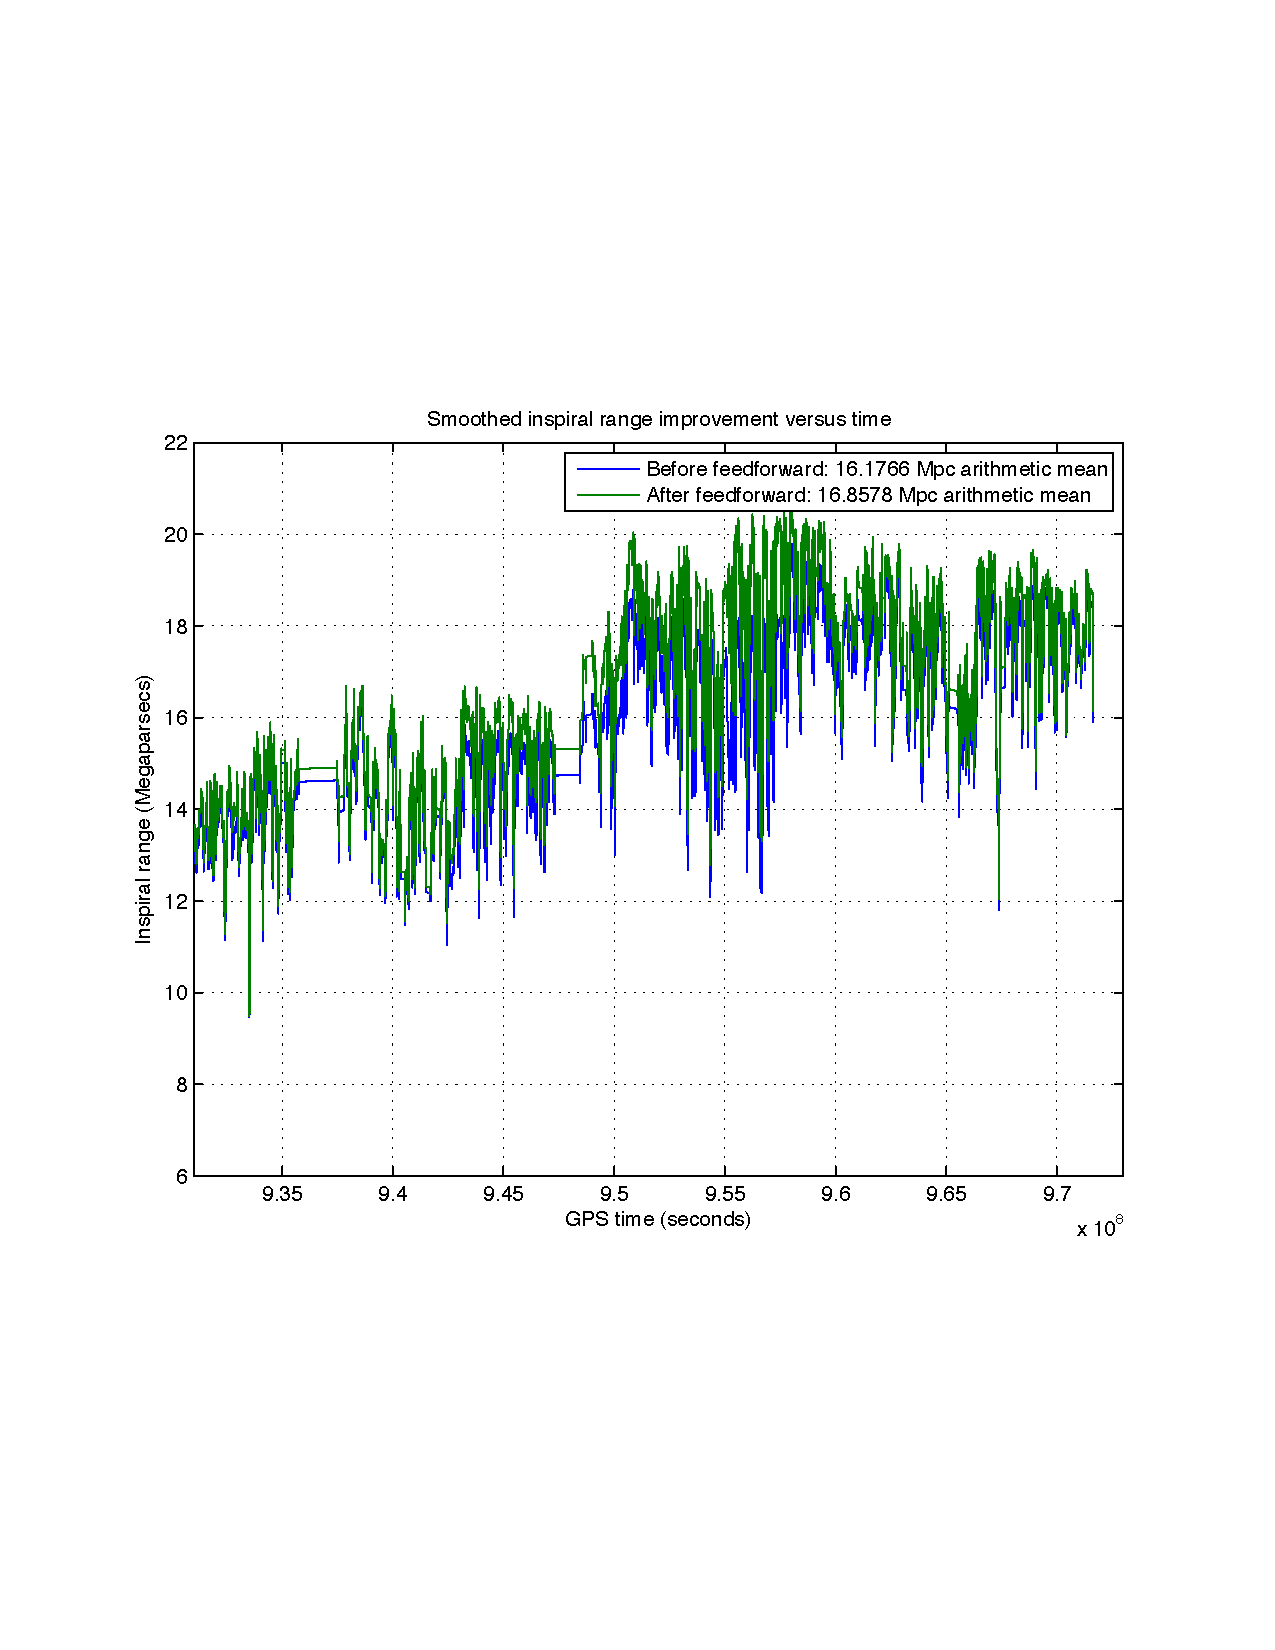
\includegraphics[width=0.45\paperwidth,height=0.6\paperheight]{plots/clip-range-LHO-new}\protect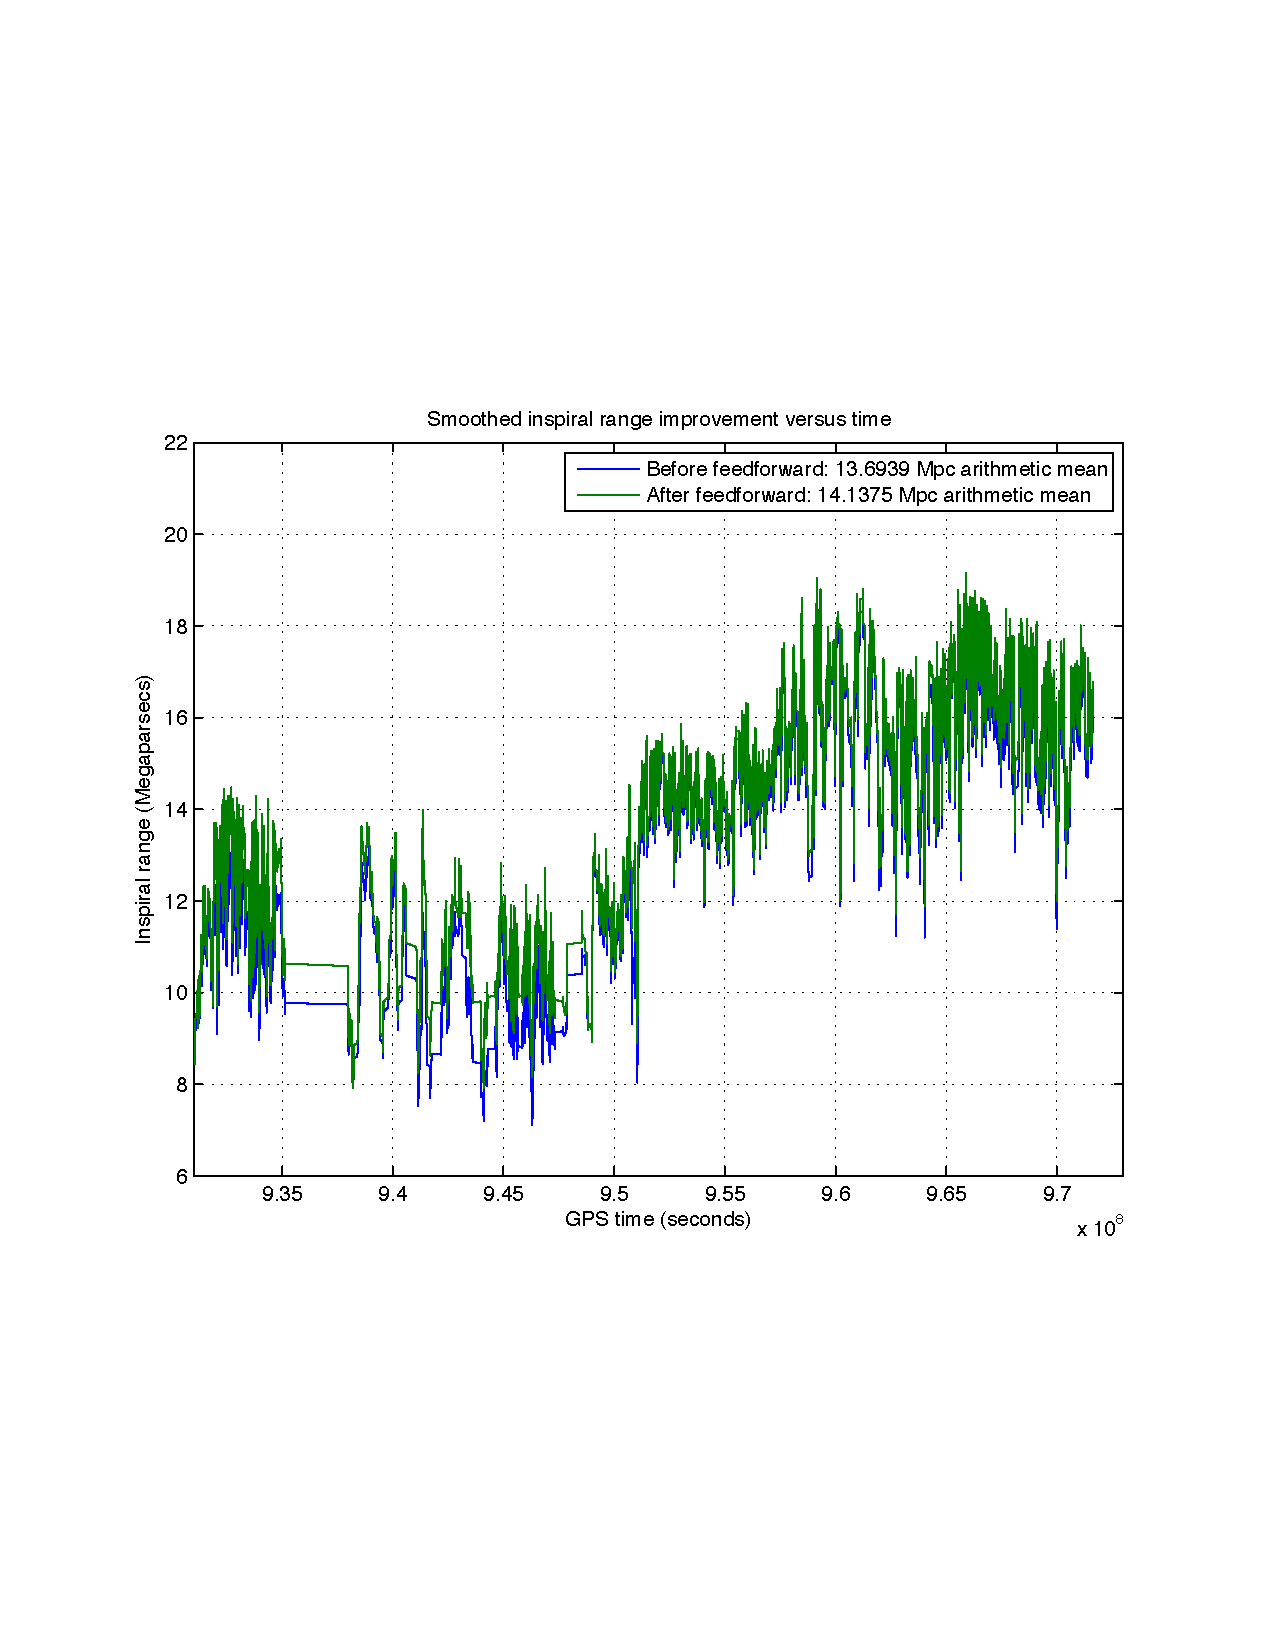
\includegraphics[width=0.45\paperwidth,height=0.6\paperheight]{plots/clip-range-LLO-new}}


Inspiral range vs time for S6

H1 (L) gains 0.69 Mpc, L1 (R) gains 0.43 Mpc
\end{figure}

\end{onlyenv}%{}

\begin{onlyenv}%{}
<2>

\begin{figure}
\caption{\protect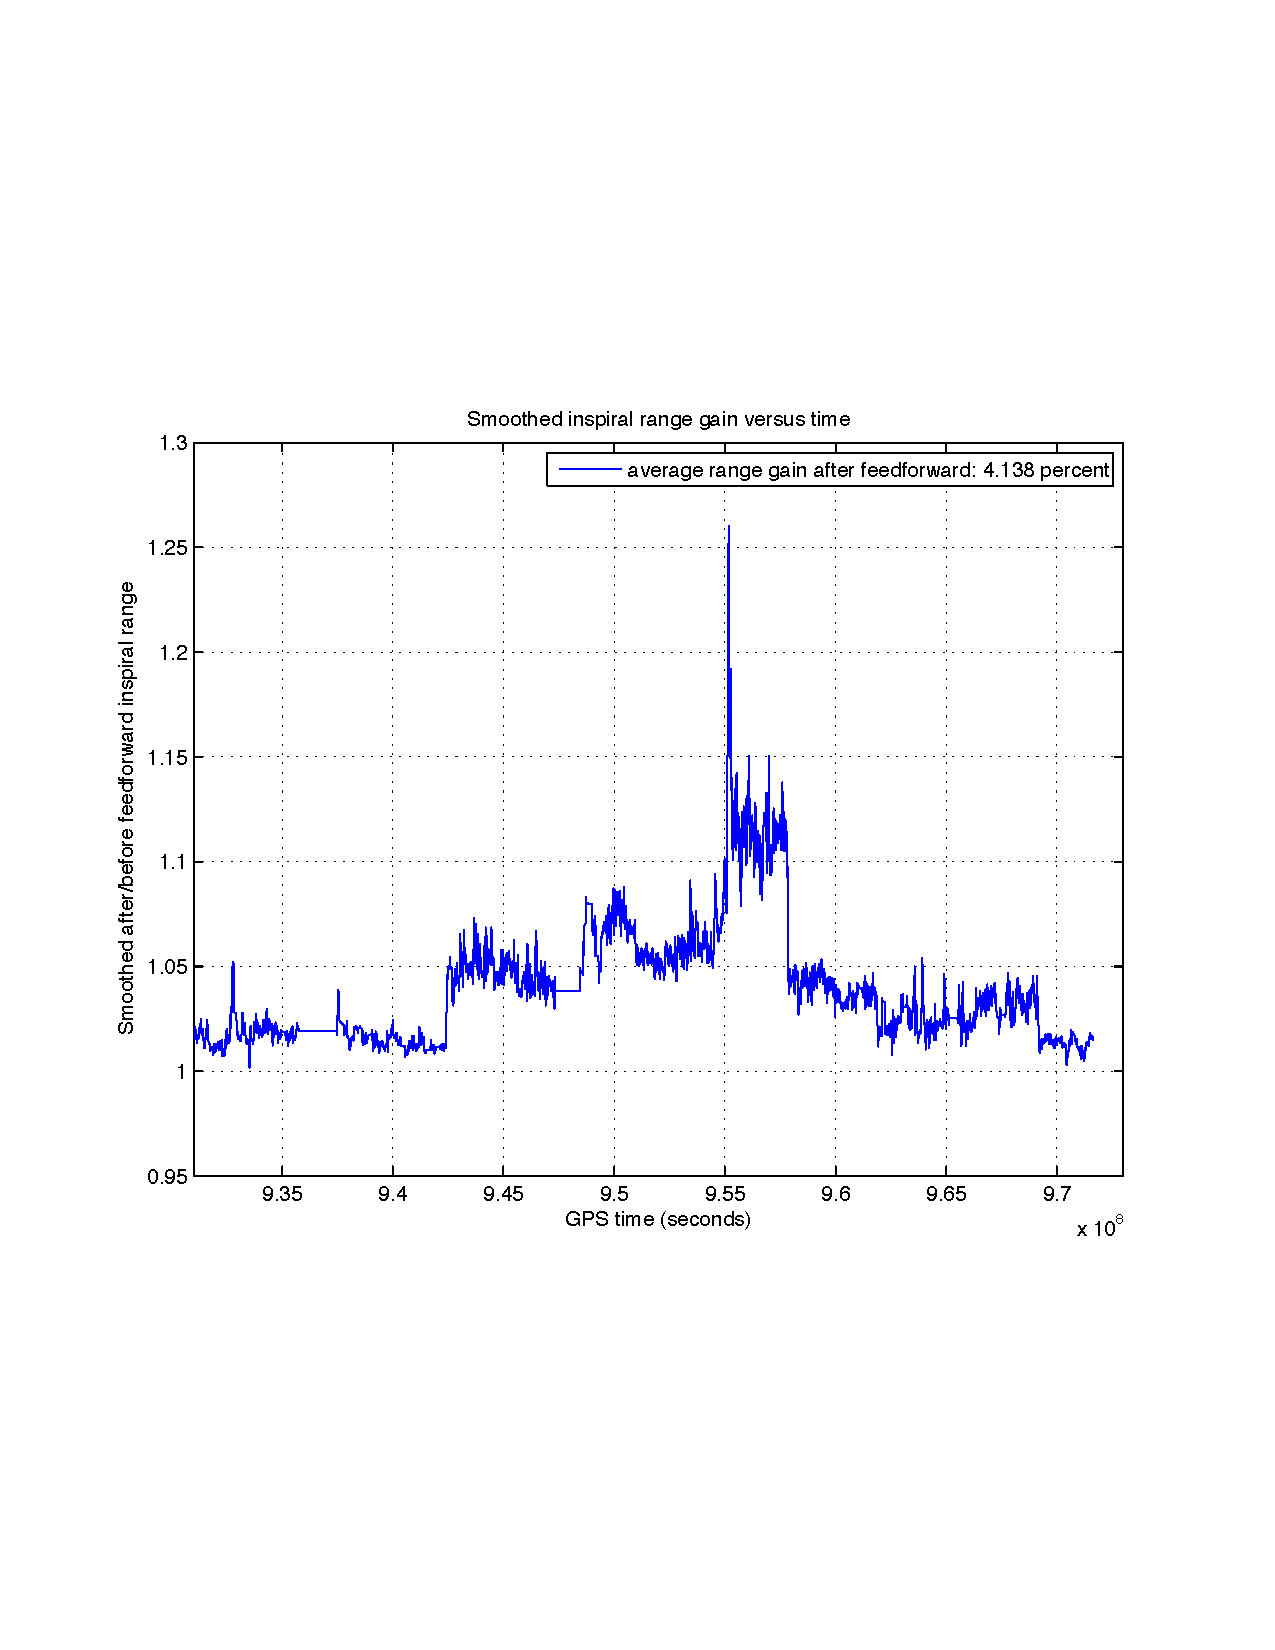
\includegraphics[width=0.45\paperwidth,height=0.6\paperheight]{plots/clip-gain-LHO-new}\protect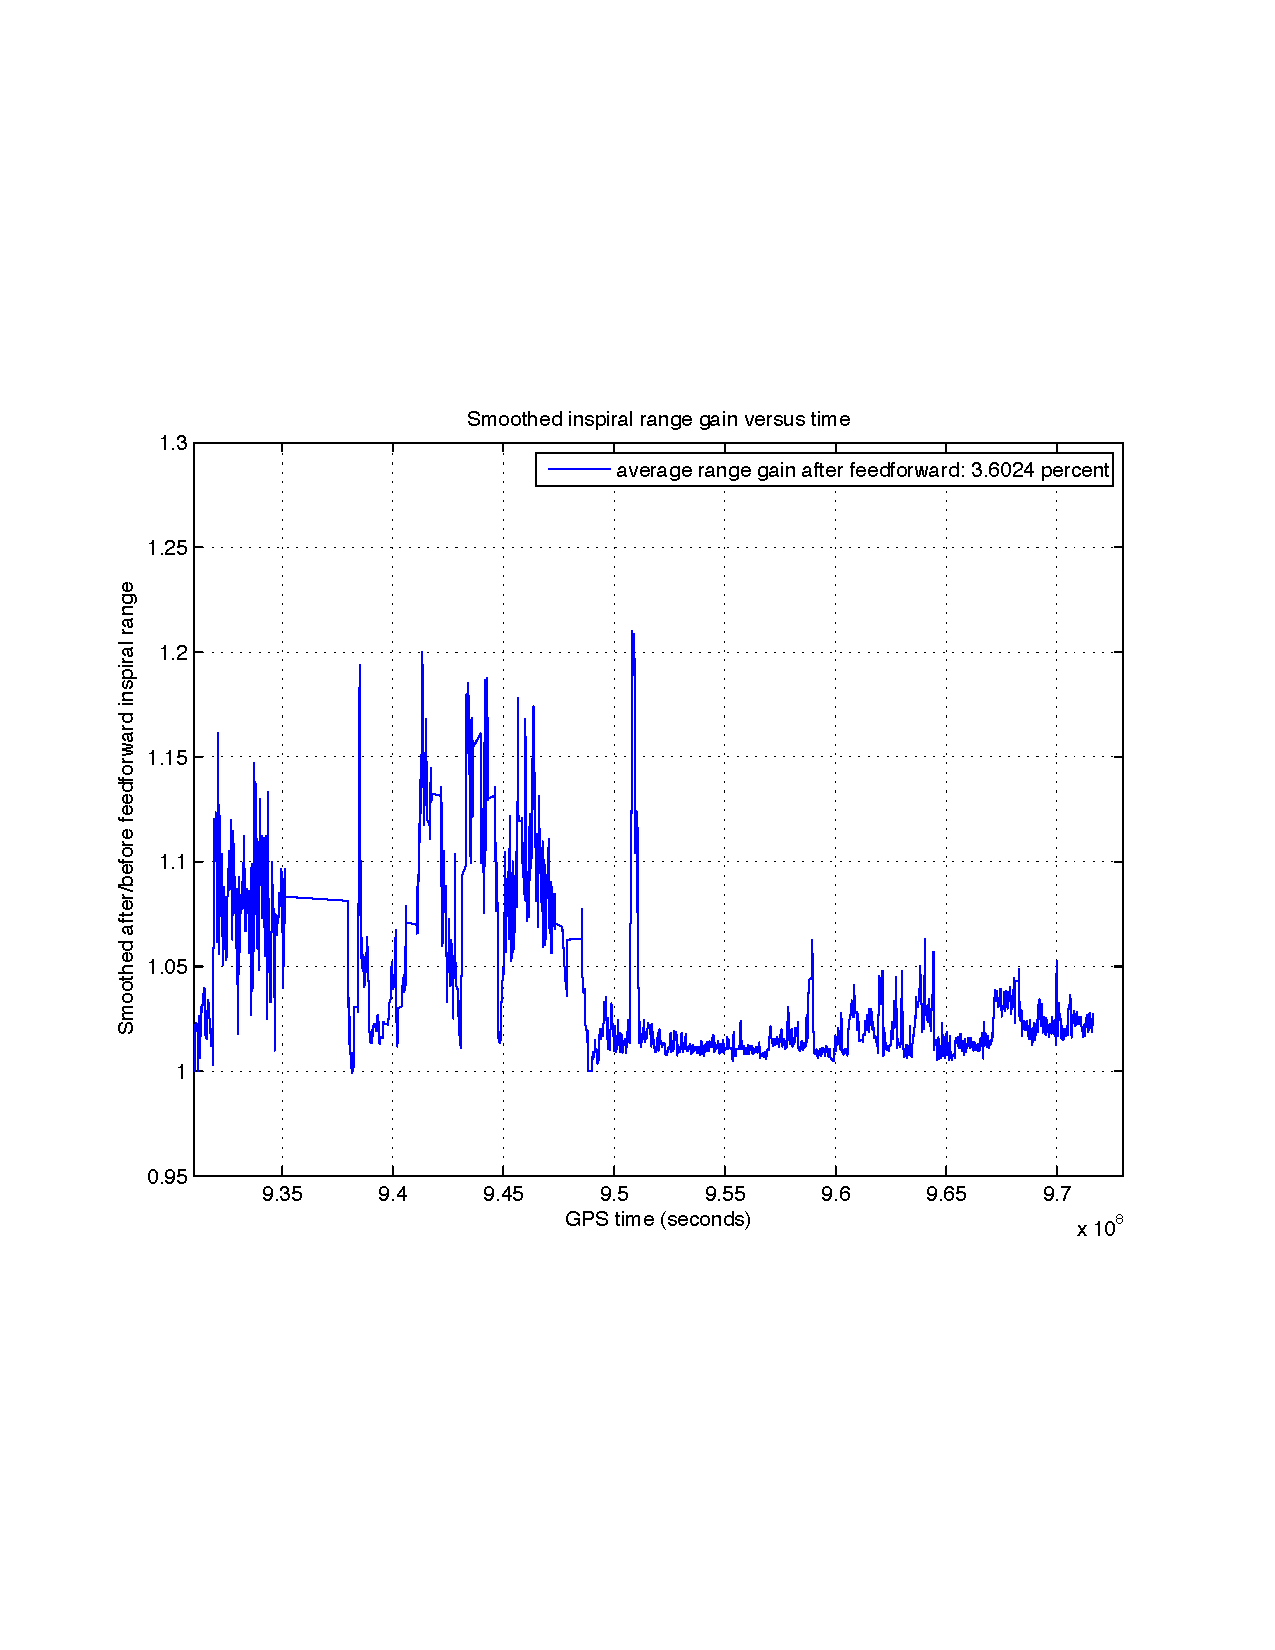
\includegraphics[width=0.45\paperwidth,height=0.6\paperheight]{plots/clip-gain-LLO-new}}


Inspiral range \emph{fractional gain} vs time for S6

H1 (L) 4.13\% better, L1 (R) 3.60\% better
\end{figure}

\end{onlyenv}%{}

%\begin{onlyenv}%{}
%<3>
%
%\begin{figure}
%\caption{\protect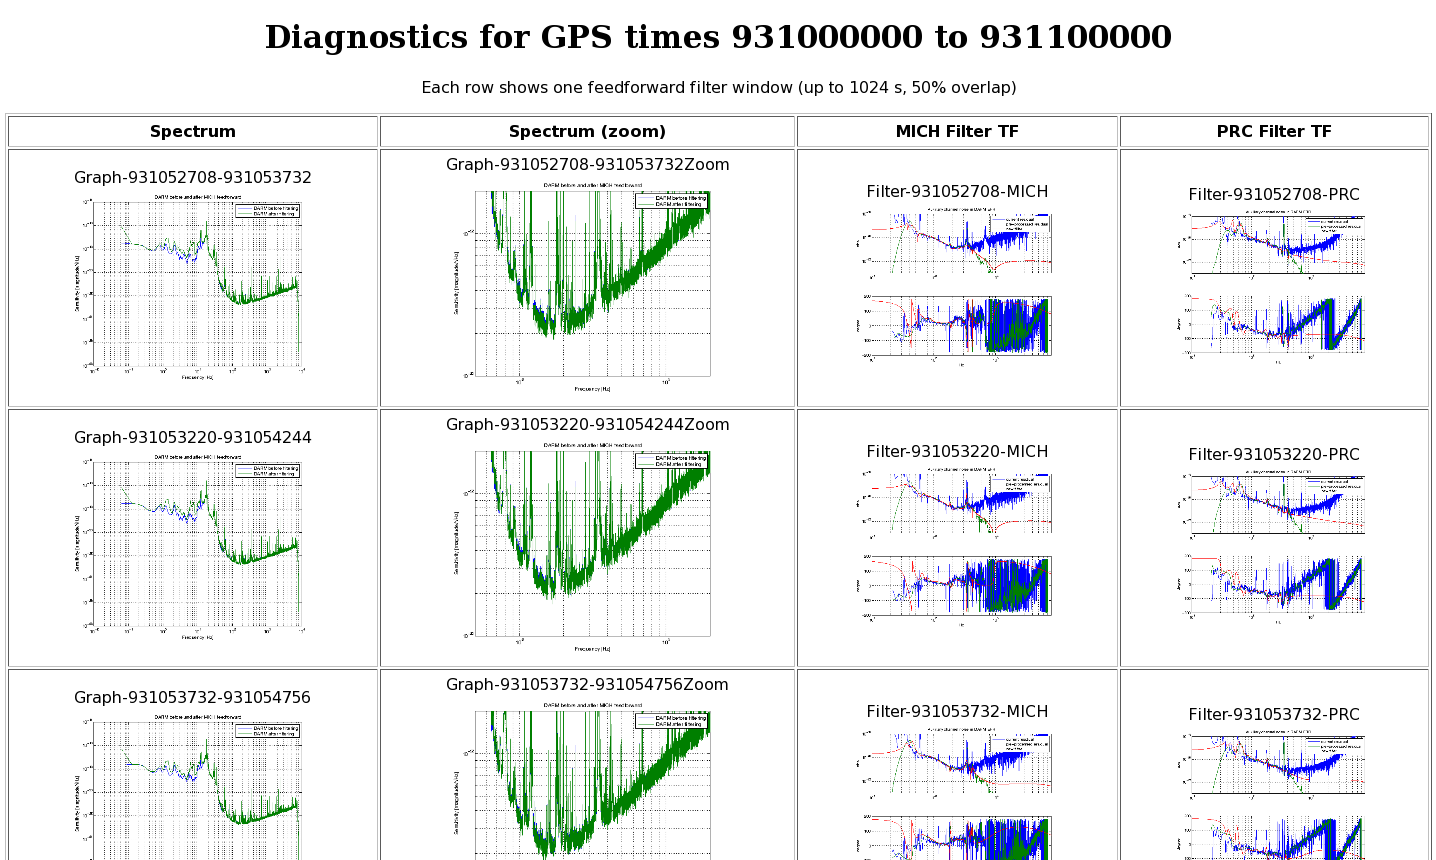
\includegraphics[height=0.62\paperheight]{croppedWebpage}}
%
%
%Webpages with window-by-window thumbnails \url{https://ldas-jobs.ligo.caltech.edu/~pulsar/feedforward/diagnostics/}
%\end{figure}

%\end{onlyenv}%{}

\lyxframeend{}\lyxframe{Timing verification: injection tests}

\begin{figure}
\caption{\protect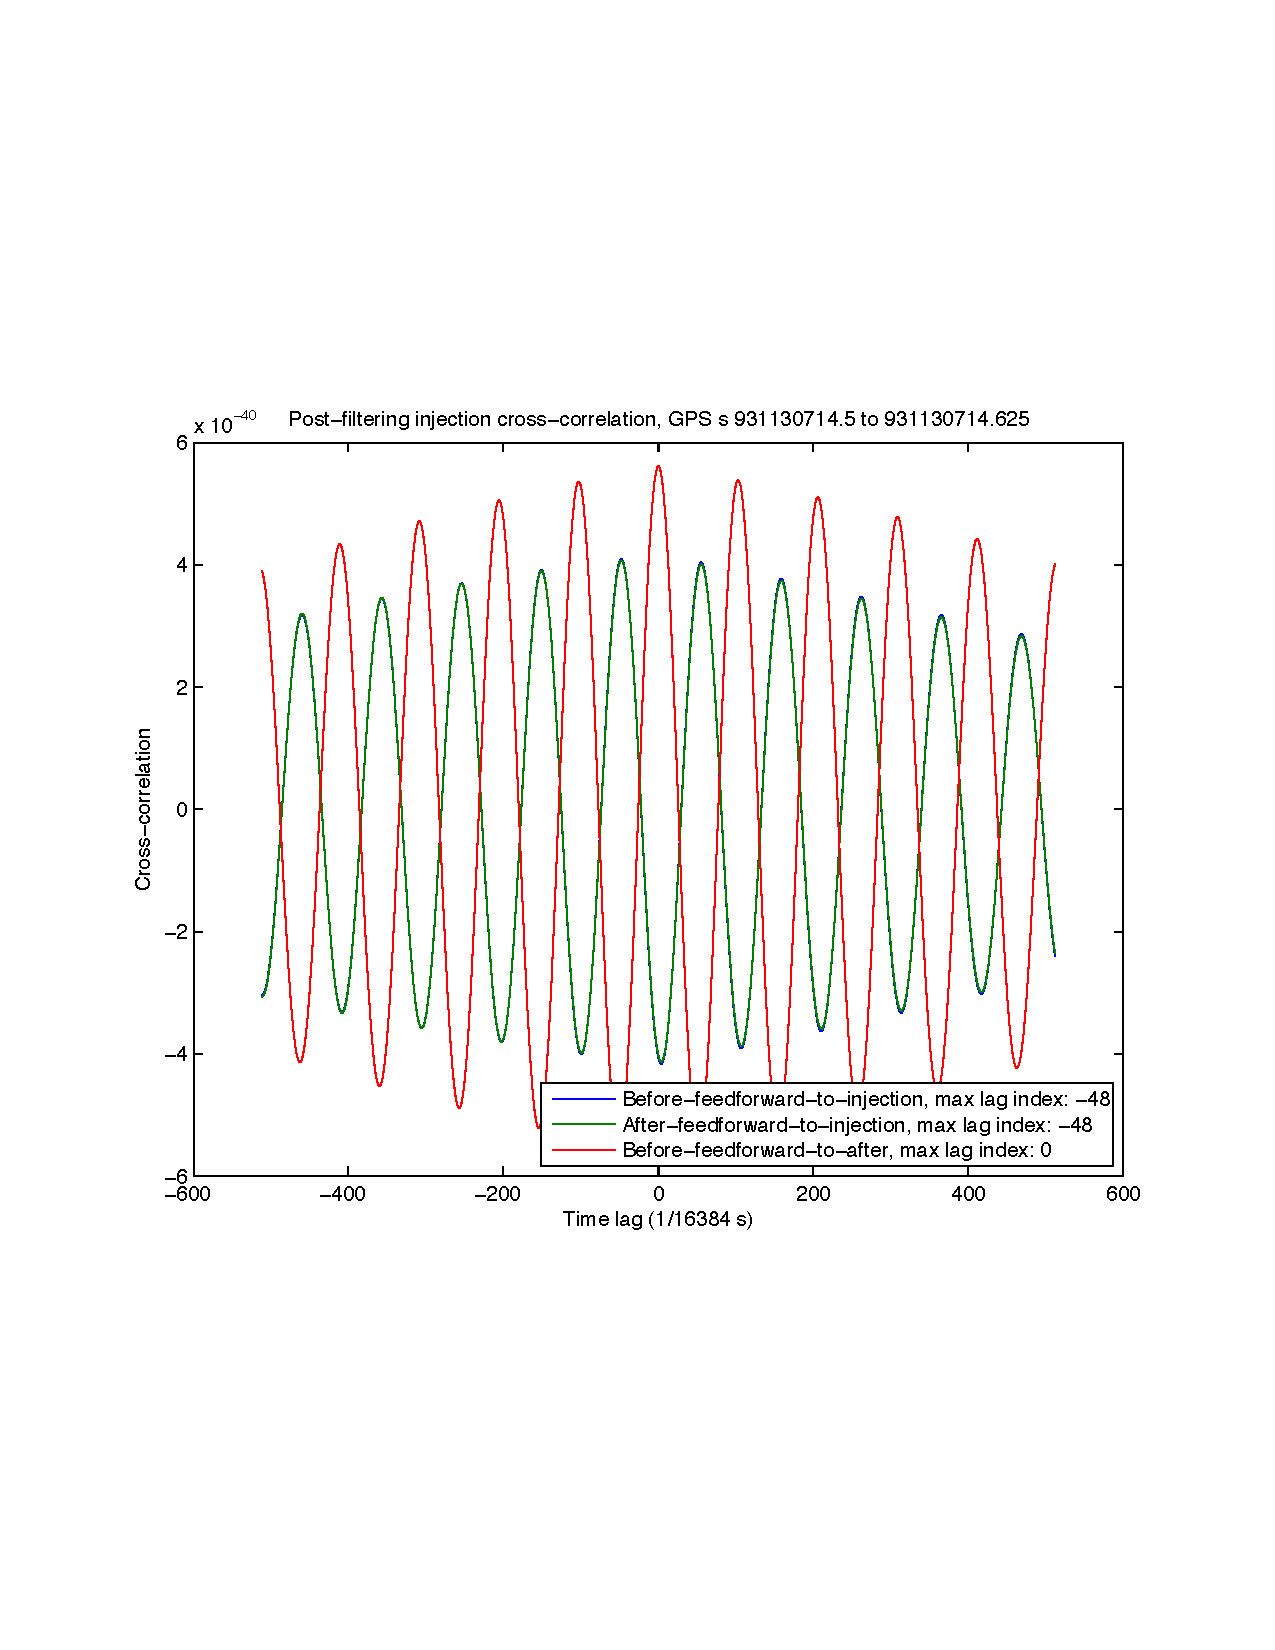
\includegraphics[width=0.45\paperwidth,height=0.6\paperheight]{plots/clip-crossCorrInjection}\protect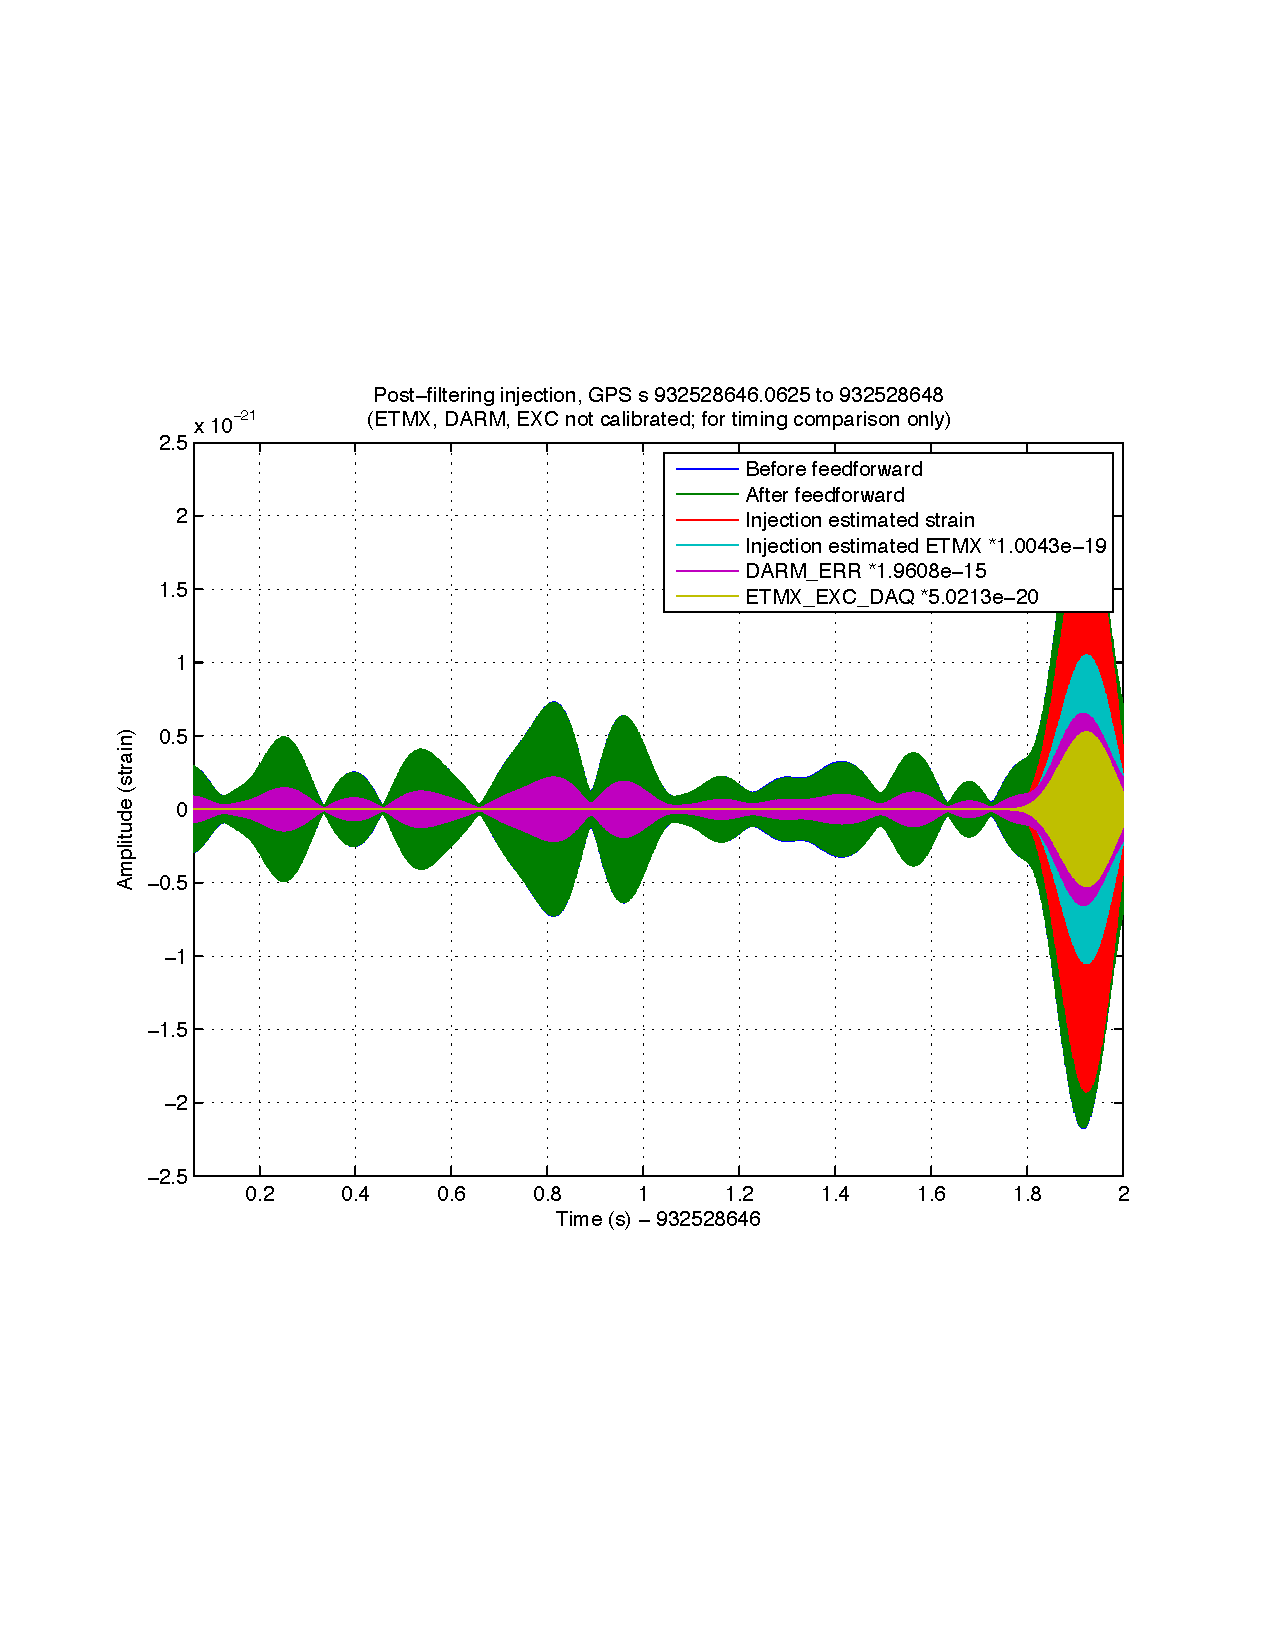
\includegraphics[width=0.45\paperwidth,height=0.6\paperheight]{plots/clip-correlateInjection}}


Cross-correlation (L) and amplitude vs time (R)

comparing before and after feedforward with

injections on ETMX (tested ringdown and sine-gaussian)
\end{figure}



\lyxframeend{}\lyxframe{Frequency verification: clean spectral peaks}

\begin{figure}
\caption{\protect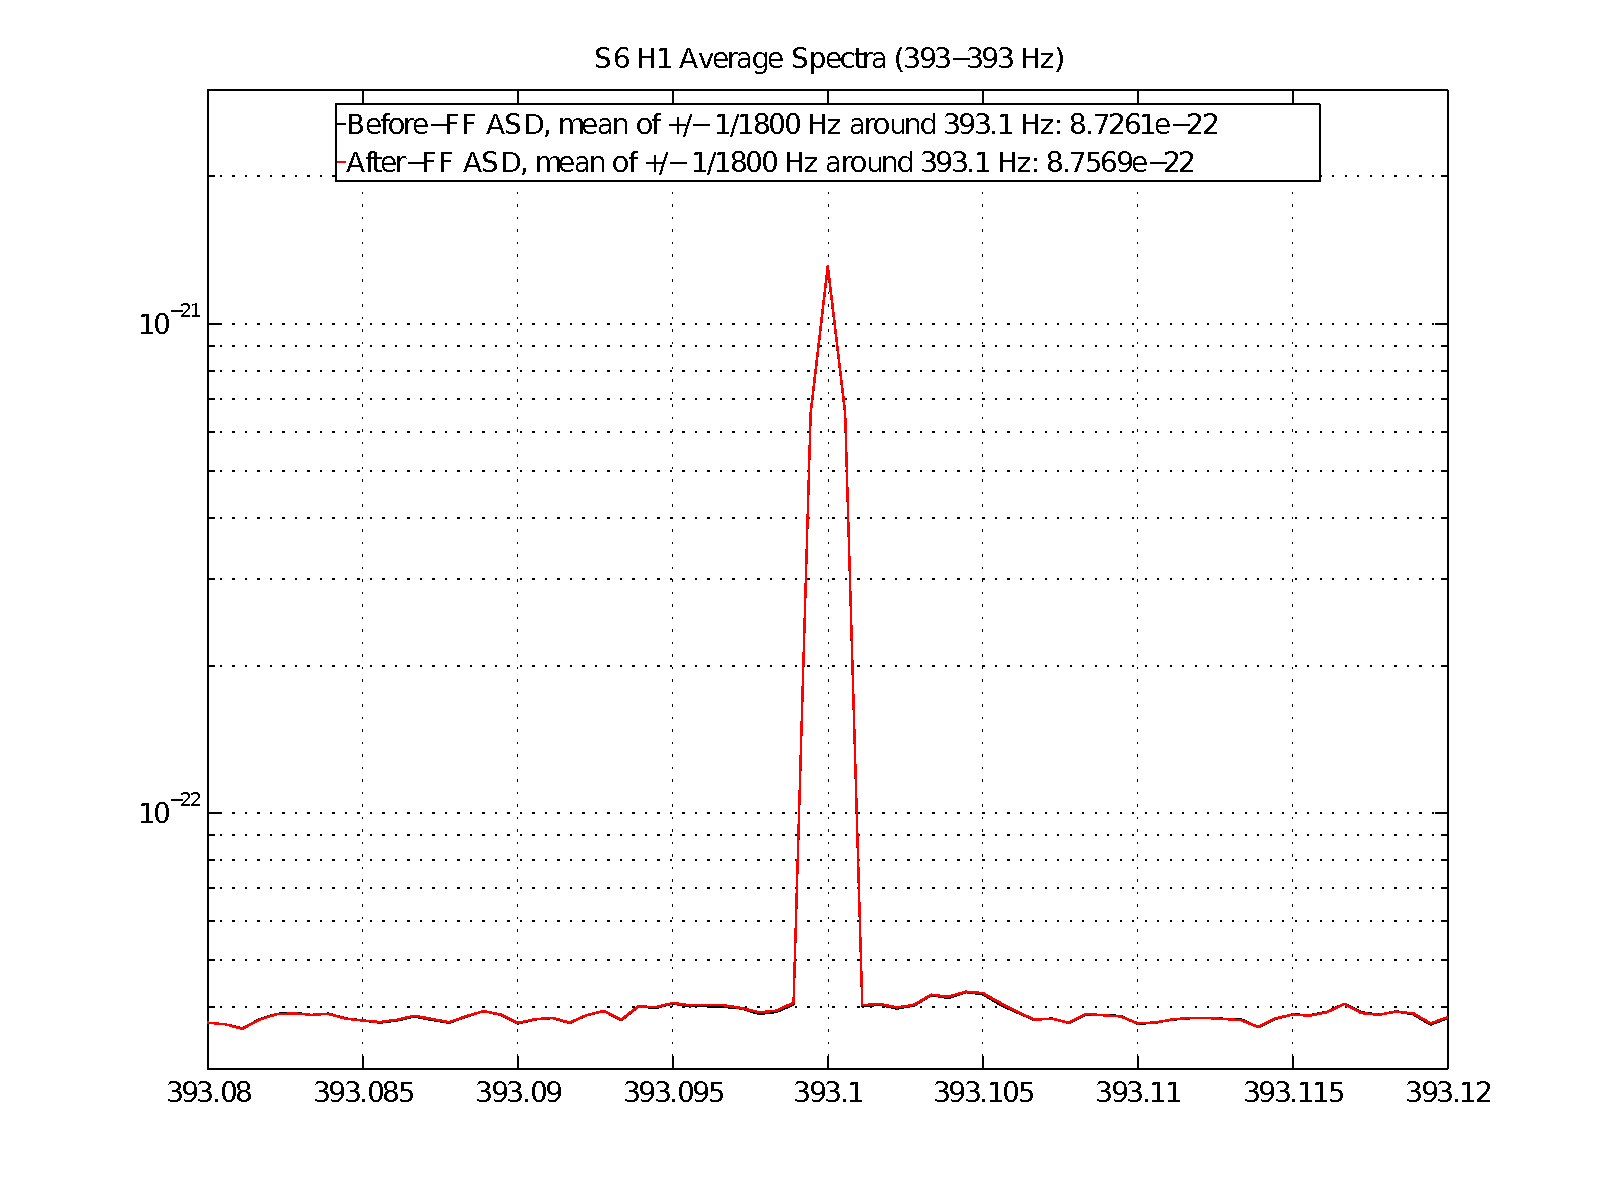
\includegraphics[width=0.9\paperwidth,height=0.5\paperheight]{plots/figure6}}


200 job harmonic mean ASD vs frequency

calibration line at 393.1 Hz shows

clean spectral peak, no comb observed

(hypothetically induced by windowing)
\end{figure}



\lyxframeend{}\section{Auxiliary filtering summary}


\lyxframeend{}\lyxframe{Auxiliary filtering summary }

\emph{Filtering summary}
\begin{enumerate}
\item h(t) filtered w/ MICH \& PRC, range +4\% (volume 12\%), minimum strain
about 10\% better
\item AMPS frames for S6 H1 \& L1 exist at CIT cluster: \url{/archive/frames/S6/pulsar/feedforward/}
\item \emph{Best} h(t) \& inspiral range of any site/time till Advanced
LIGO
\item Advanced LIGO: characterize MICH \& PRC changes, fix quickly, even
\emph{post facto}
\end{enumerate}
\emph{Filtering acknowledgments}

K. Kawabe, K. Riles, G. Mendell; National Science Foundation, LIGO
Scientific Collaboration, LIGO Hanford Observatory, and U. of Michigan;
method after Allen, Hua and Ottewill.


\lyxframeend{}\section{Searches for neutron stars in binary systems}


\lyxframeend{}\lyxframe{TwoSpect algorithm for all-sky binary searches}

\textbf{TwoSpect} (Goetz \& Riles 2011) searches for patterns in

doubly Fourier-transformed data from binary's orbital modulation

\emph{doubly Fourier-transformed:} $k$ frequency bins, time series
$n$

Short Fourier Transform series, along $n$, is FFT'd 

\[
R=\frac{\Sigma_{i=0}^{M-1}w(m_{i})[Z(m_{i})-\lambda(m_{i})]}{\Sigma_{i=0}^{M-1}[w(m_{i})]^{2}}
\]


$R$: template detection statistic

$w$: template weight

$i$: pixel index of $M$ pixels

$Z$: spectral power (after barycentric correction)

$\lambda$: expected noise power

$\rightarrow$ E. Goetz wrote, conducting all-sky search

\lyxframeend{}\lyxframe{TwoSpect algorithm for all-sky binary searches}

\begin{figure}
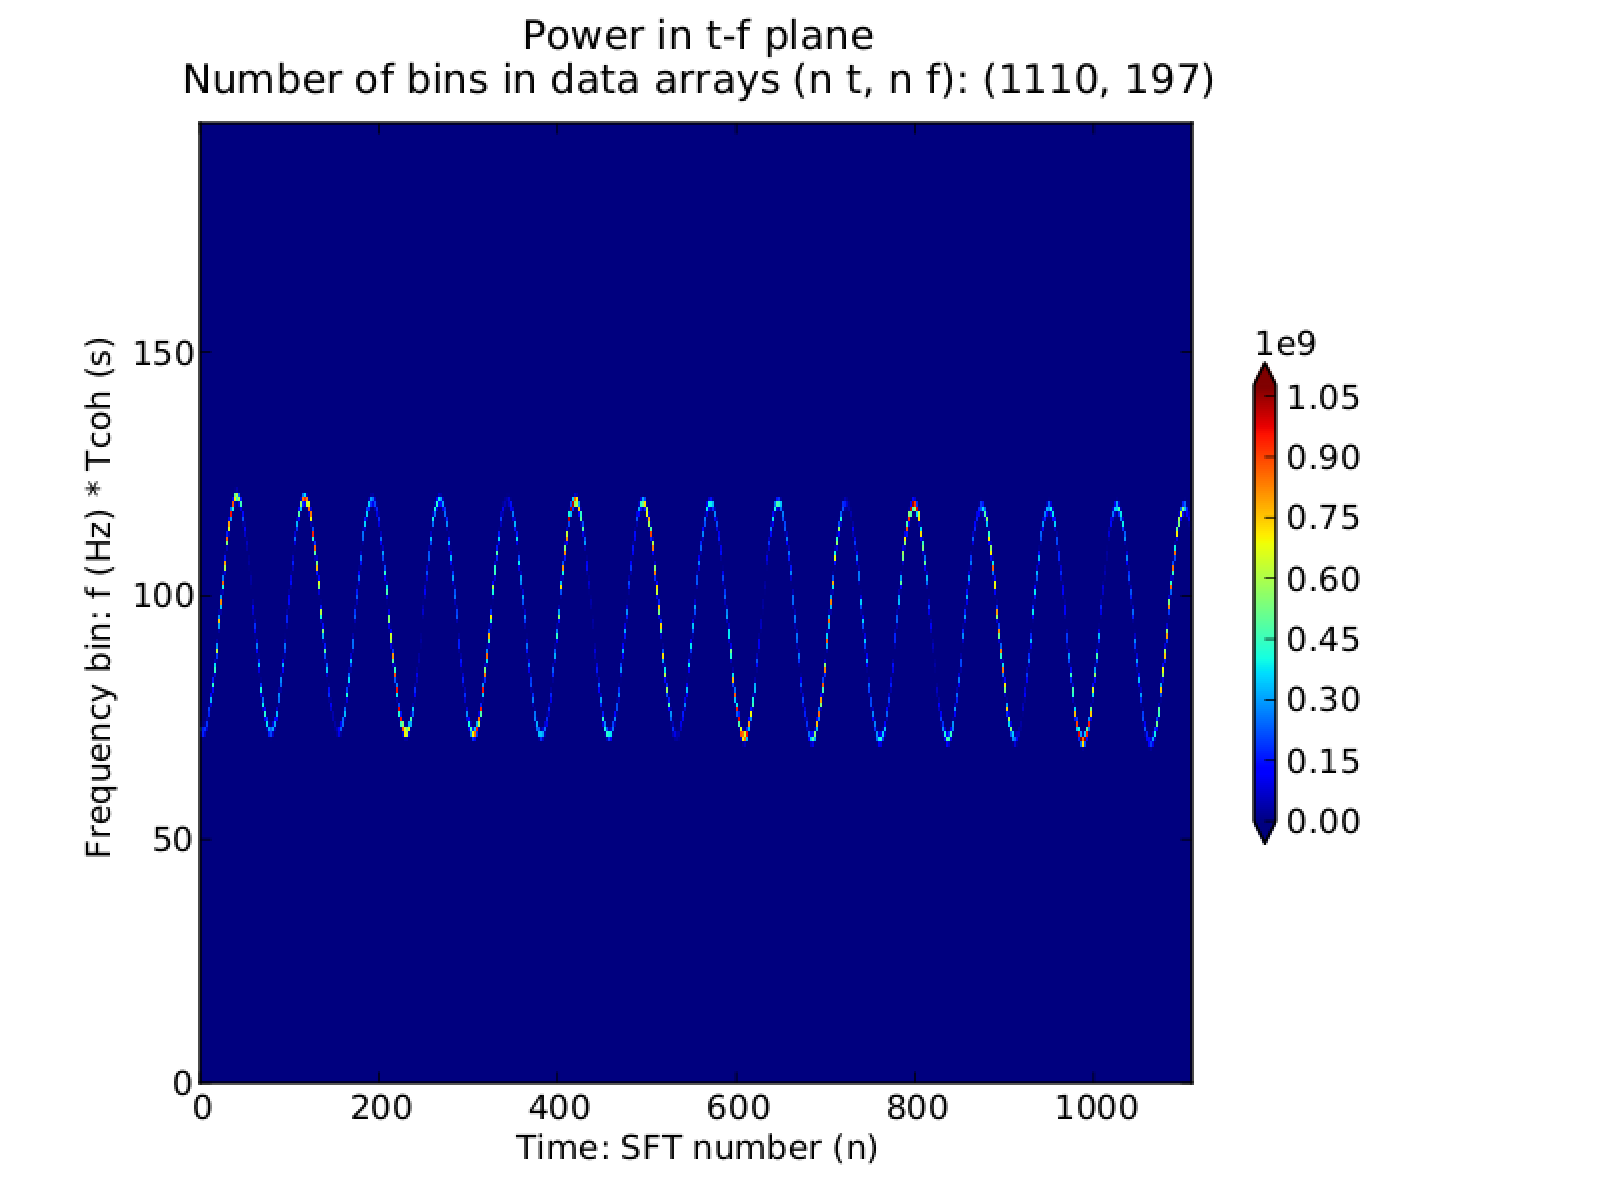
\includegraphics[width=0.48\paperwidth]{plots/tfplane-4e21-on-4e24.png}
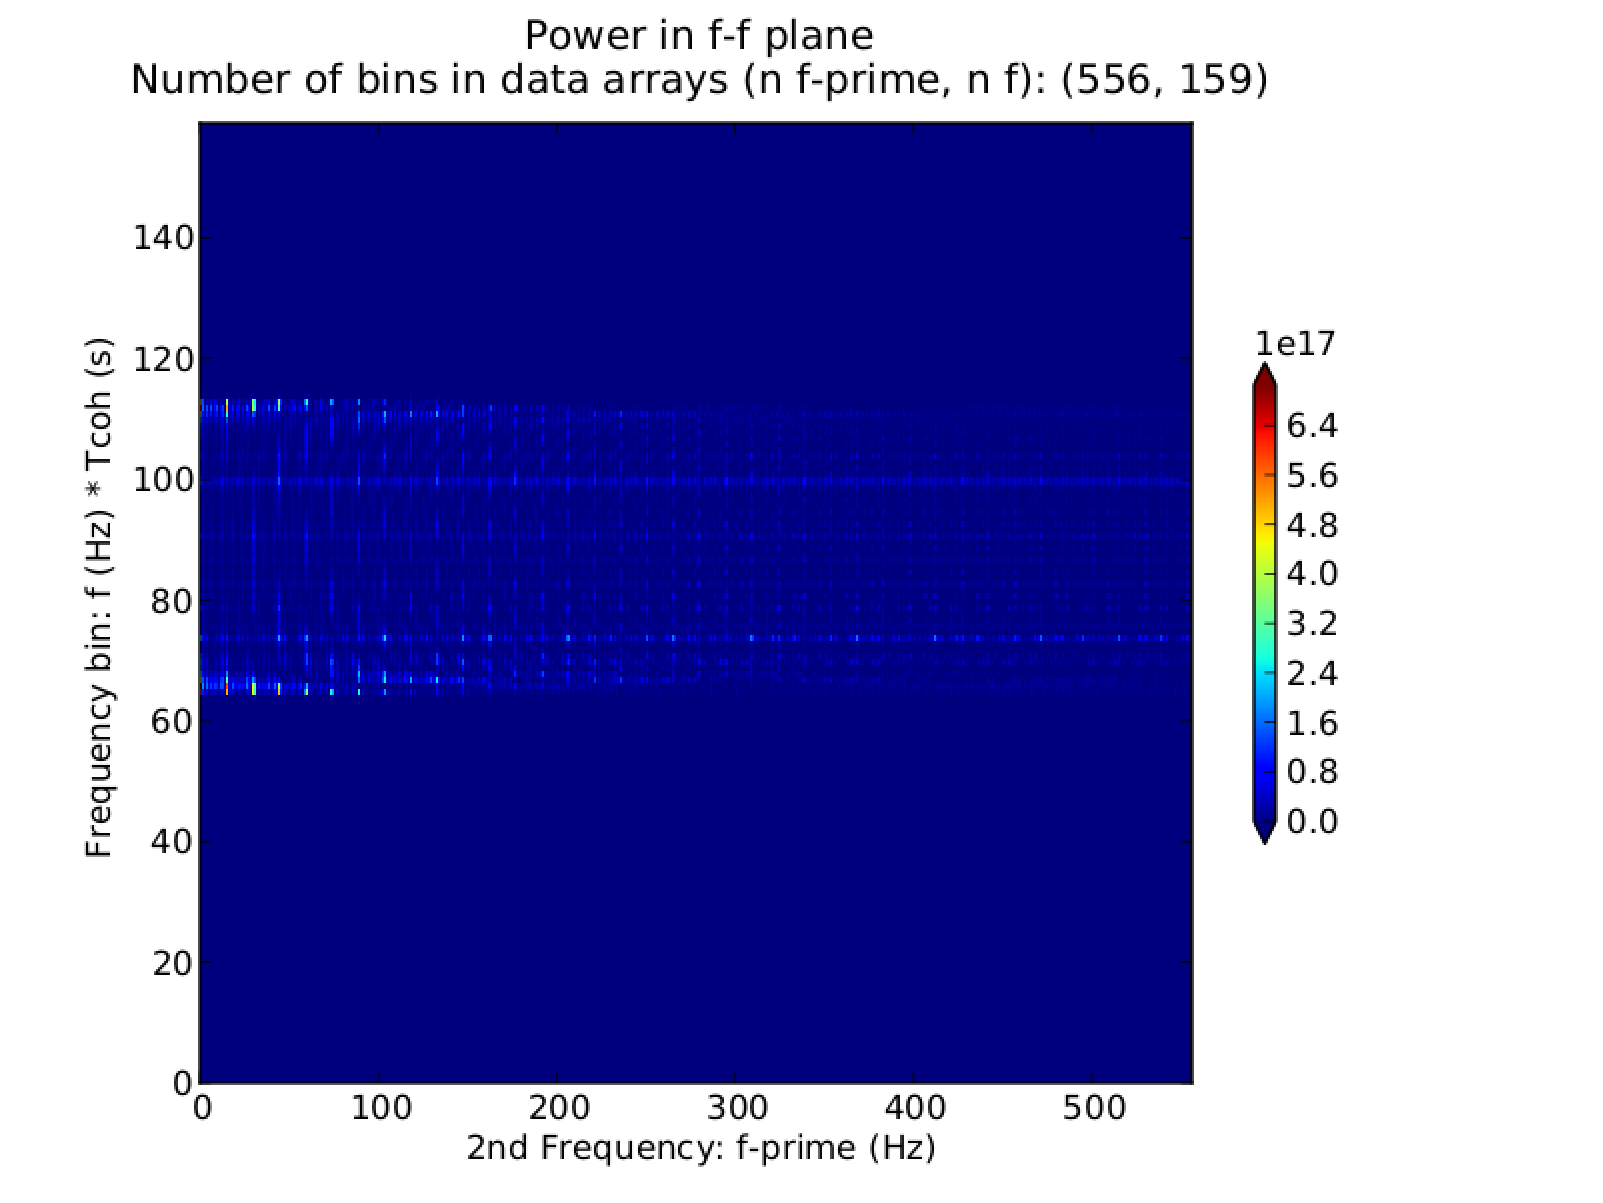
\includegraphics[width=0.48\paperwidth]{plots/ffplane-4e21-on-4e24.png}
\caption{Time-frequency spectogram (LEFT) is Fourier-transformed along SFT number into frequency-frequency spectogram (RIGHT), which is matched against putative signal templates }
\end{figure}


\lyxframeend{}\lyxframe{Directed TwoSpect's greater sensitivity}

\emph{All-sky search: }parameter space $\gg10^{18}$ templates
\begin{itemize}
\item Hierachical search; incoherent harmonic sum to consolidate\\
parameter space, use templates to test interesting outliers
\end{itemize}
\emph{Directed search: }parameter space much smaller
\begin{itemize}
\item Fully template the parameter space for max sensitivity
\end{itemize}

\[
\begin{split}
N_{\textup{{template}}} &=\left[1+2f_{bw}T_{coh}\right] \times \ldots \\
& \left[ {\displaystyle \Sigma}_{j=1}^{j = \frac{f_{max} - f_{min}}{f_{bw}}} 1 + 2\pi\left(f_{min} + j f_{bw}\right) \frac{4 T_{coh}}{P} 6 \sigma_{a \sin i} \right],
\end{split}
\]

\noindent search at one IFO over $\pm 3 \sigma$ around $a\sin i$ to simplify,

\[
\begin{split}
N_{\textup{template}} &= 2 \left(T_{coh} + \frac{1}{f_{bw}}\right) \times \ldots \\
& \left[ 1+ \frac{4 \pi T_{coh}}{P} (6\sigma_{a \sin i})(f_{max} + f_{min} + f_{bw})\right] 
 (f_{max} - f_{min})
\end{split}
\]

%\[
%N_{\textup{{template}}}=(f_{max}-f_{min})(2T_{coh}){\displaystyle \Sigma}_{f_{min}}^{f_{max}}(2\pi f)(4T_{coh})\frac{a\sin\iota}{P}
%\]



\lyxframeend{}\lyxframe{Directed TwoSpect's greater sensitivity}

\textbf{Scorpius X-1 (P $\approx$$ $ 68023.7 s, $a \sin i$ $\approx1.44\pm0.18$s):}
\begin{itemize}
\item $N_{template}\approx10^{8}$ for 3 interferometers\\(500 Hz band; $3\sigma$
in $a\sin i$)$ $
\item Tractable to test all templates$\rightarrow$ need new methods
\end{itemize}

$\textup{}$

\textbf{Test methods in Mock Data Challenge (MDC)}
\begin{itemize}
\item TwoSpect is 1 of up to 6 algorithms looking for \\
50 ``open'', 50 ``closed/blind'' Sco X-1-like ``pulsars'' (LMXBs)
\end{itemize}

\lyxframeend{}\section{Scorpius X-1 mock data challenge}


\lyxframeend{}\lyxframe{Fully-templated search for Scorpius X-1}

\begin{figure}
\caption{\protect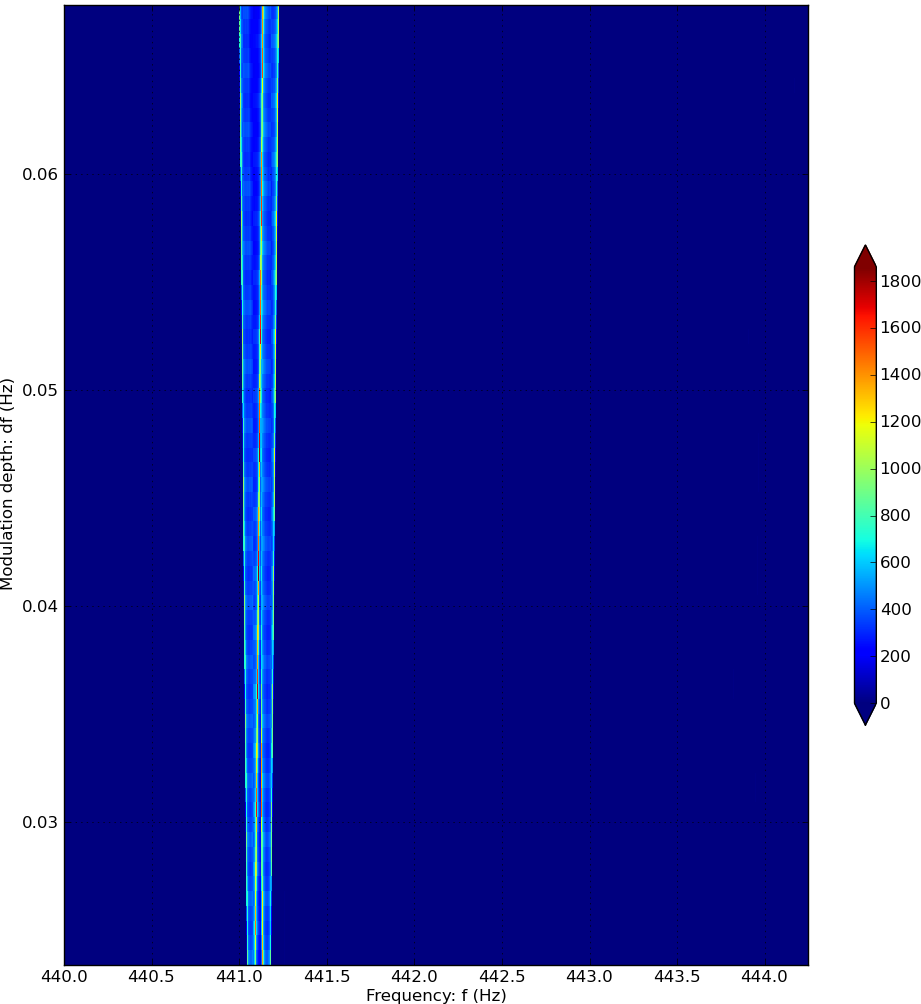
\includegraphics[width=0.8\paperwidth,height=0.62\paperheight]{plots/bandH1-bold}}


\textbf{Scorpius X-1 MDC ``pulsar 40'' \{H1\} 5 Hz band}

p-value (based on R statistic) in red

all (frequency, modulation depth) templates
\end{figure}

\lyxframeend{}\lyxframe{Wide-band heat maps in parameter space}

\begin{figure}
\caption{\protect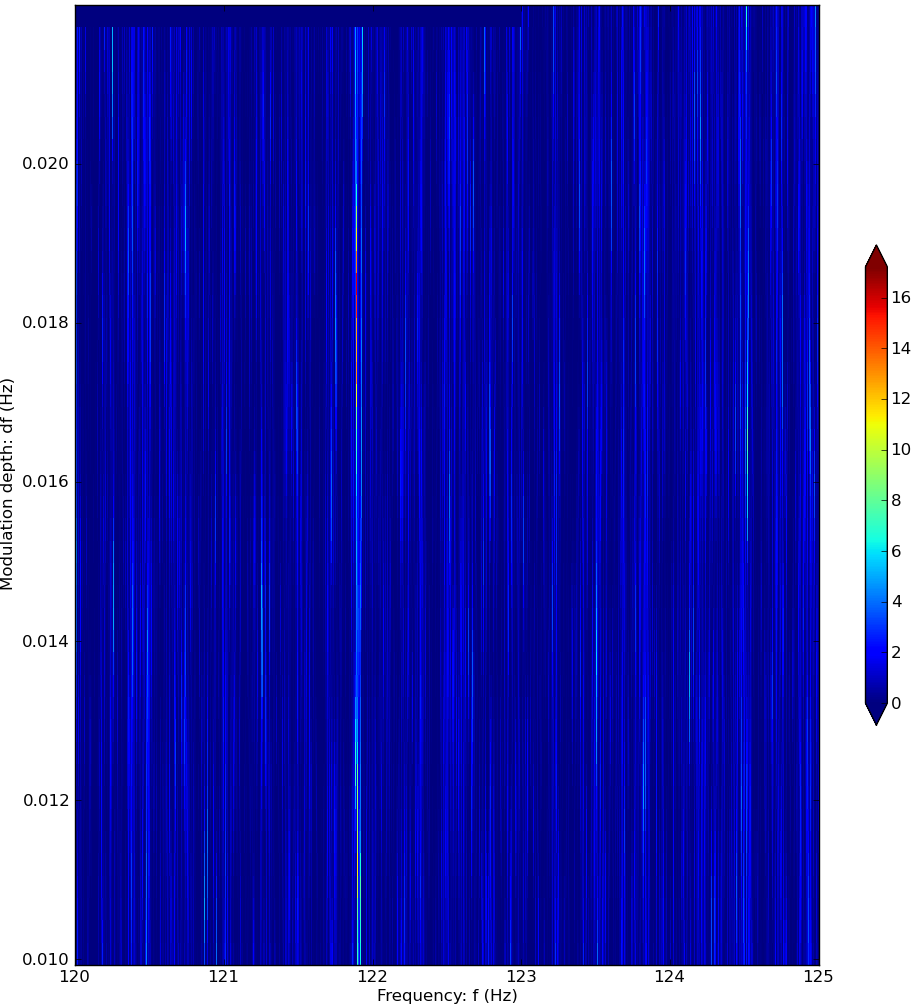
\includegraphics[width=0.8\paperwidth,height=0.62\paperheight]{plots/bandH1}}


\textbf{Scorpius X-1 MDC ``pulsar 8'' \{H1\} 5 Hz band}

$3.6\times10^{5}$ templates, 10-22 mHz mod. depth, 120-125 Hz frequency

Signal at about (df = 0.019, f = 121.9) Hz
\end{figure}



\lyxframeend{}\lyxframe{Narrow-band heat maps in parameter space}

\begin{figure}
\caption{\protect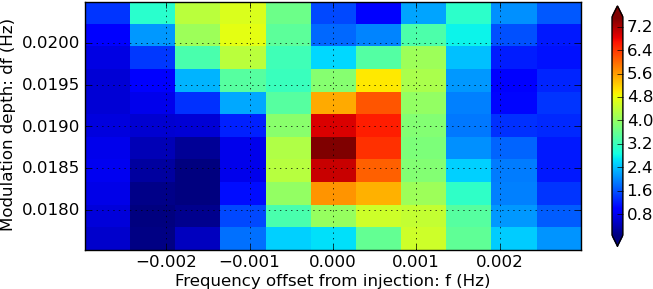
\includegraphics[width=0.4\paperwidth,height=0.2\paperheight]{plots/heatmapH1}}
\caption{\protect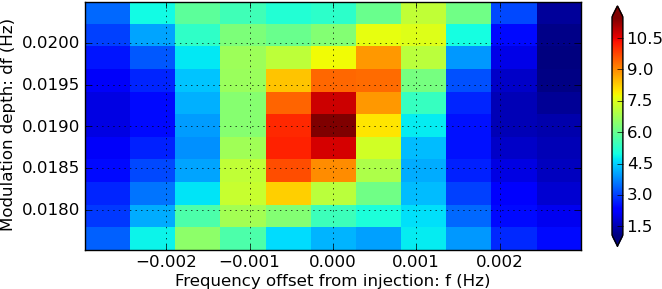
\includegraphics[width=0.4\paperwidth,height=0.2\paperheight]{plots/heatmapL1}}
\caption{\protect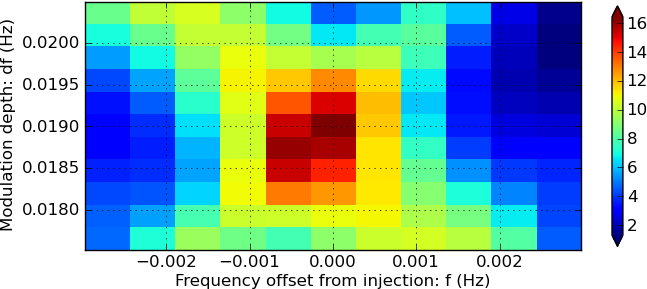
\includegraphics[width=0.4\paperwidth,height=0.2\paperheight]{plots/heatmapV1}}
Heatmaps \{H1, L1, V1\} of 11x11 templates centered around
\textbf{Scorpius X-1 MDC ``pulsar 8''}
\end{figure}






\lyxframeend{}\lyxframe{Revisiting \& refining detection criteria}

Used MDC band \textbf{Gaussian noise}, affected by time gaps\\

\begin{figure}
\caption{\protect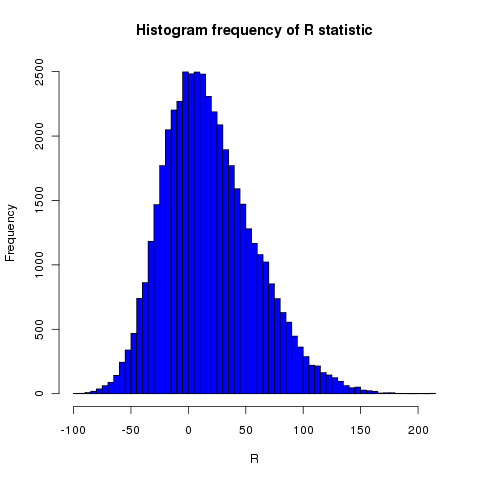
\includegraphics[width=0.45\paperwidth,height=0.45\paperheight]{plots/StatHistRH1}\protect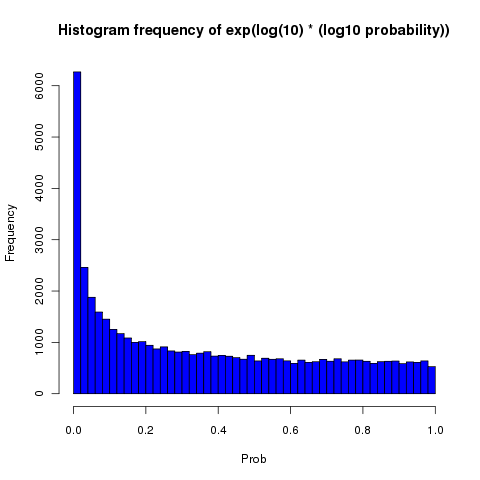
\includegraphics[width=0.45\paperwidth,height=0.45\paperheight]{plots/StatHistProbH1}}
established signal \emph{threshold log10p-values}:\\
 -7.75 in 840 s SFTs, -12.0 in 360 s SFTs $\sim$ 1\% false alarm / 5 Hz \\
(p-value differed from all-sky -- trials factor)
\end{figure}

\lyxframeend{}\section{Mock data challenge statistics}


\lyxframeend{}\lyxframe{Mock data challenge: correcting for unknown cos $\iota$}

Circular effective $h_0 = h_0 [( [(1+\cos^2 \iota)/2]^2 + [\cos \iota]^2)/2]^{1/2}$

\begin{figure}
\caption{\protect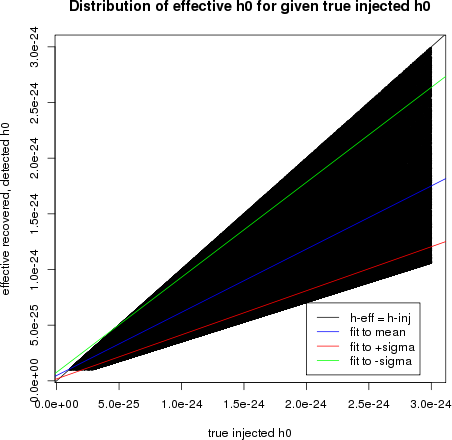
\includegraphics[width=0.45\paperwidth,height=0.45\paperheight]{plots/PlotHEffVsH0TrueWithLines.png}\protect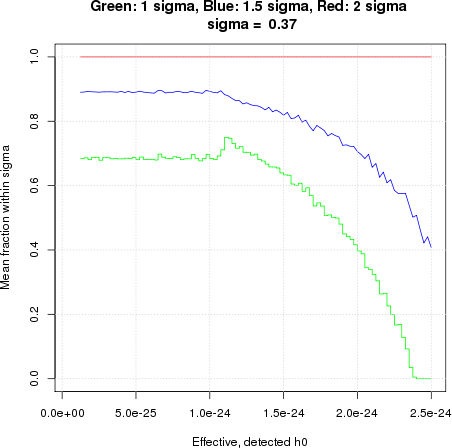
\includegraphics[width=0.45\paperwidth,height=0.45\paperheight]{plots/PlotSigmaDiffVsH0Eff.png}}
(LEFT) simulated 2 million stars with random $\cos \iota$ values\\
(RIGHT) given mean recovered/injected $h_0$, \\found relative uncertainty $\sigma$
\end{figure}

\lyxframeend{}\lyxframe{Mock data challenge: $h_0$ recovered vs injected}

\begin{figure}
\caption{\protect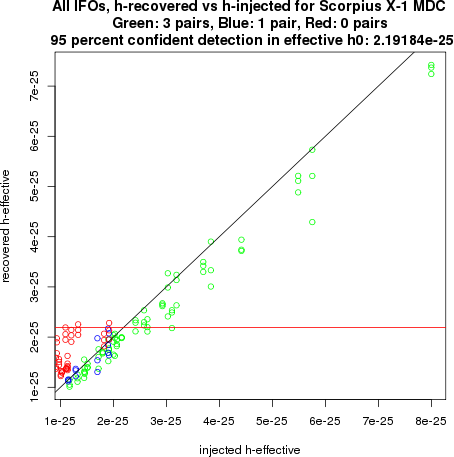
\includegraphics[width=0.7\paperwidth,height=0.7\paperheight]{plots/HrecoveredVsHeffectiveFullUL.png}}
Recovered vs circular-effective injected $h_0$ values,\\
non-detected shelf sets upper limit for $4.0 \times 10^{-24}$ noise
\end{figure}

\lyxframeend{}\lyxframe{Mock data challenge: parameter estimation, $f$}

\begin{figure}
\caption{\protect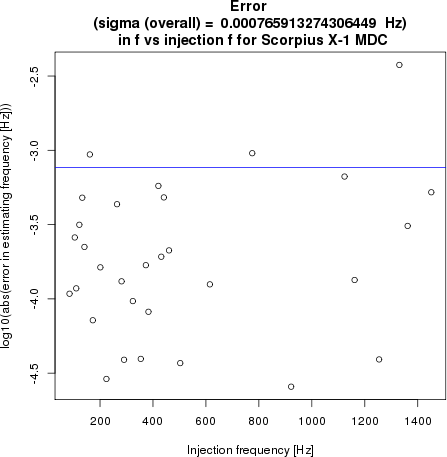
\includegraphics[width=0.7\paperwidth,height=0.7\paperheight]{plots/ErrorFvsF.png}}
Error in open-pulsar estimation of $f$, plotted vs $f$,\\
sigma based on all detected open injections
\end{figure}

\lyxframeend{}\lyxframe{Mock data challenge: parameter estimation, $a \sin i$}

\begin{figure}
\caption{\protect\includegraphics[width=0.7\paperwidth,height=0.7\paperheight]{plots/ErrorAsinivsF.png}}
Error in open-pulsar estimation of $a \sin i$, plotted vs $f$,\\
sigma based on all detected open injections
\end{figure}

\lyxframeend{}\lyxframe{Mock data challenge: parameter estimation, $h_0$}

\begin{figure}
\caption{\protect\includegraphics[width=0.7\paperwidth,height=0.7\paperheight]{plots/Errorh0vsF.png}}
Error in open-pulsar estimation of $h_0$, plotted vs $f$,\\
sigma based on all detected open injections
\end{figure}

\lyxframeend{}\lyxframe{Mock data challenge: results}

\emph{Scorpius X-1 MDC}
\begin{itemize}
\item 34 of 50 closed (and 31 of 50 open) pulsars detected
\item $f$, $a \sin i$ and $h_0$ estimated
\item $4.23\times 10^{-25}$ strain UL in $4 \times 10^{-24}$ strain Hz$^{1/2}$ noise
\item with injections to refine UL, applicable to real data
\end{itemize}

\lyxframeend{}\section{S6: Scorpius X-1 search plan}

\lyxframeend{}\lyxframe{S6: Scorpius X-1 search plan}

\textbf{2 kHz, $\pm 3 \sigma_{a \sin i}$ search over all S6 data from H1 \& L1}
\begin{itemize}
\item Analyze 40 to 360 Hz with 840 s SFTs,
\item Analyze 360 to 2040 Hz with 360 s SFTs,\\
(to prevent spectral leakage)
\item Also done: overlapping bands to verify
\item Search over 300+1700 Hz = 2.0 kHz complete on H1, L1
\end{itemize}

\lyxframeend{}\section{Real S6 data: statistics}
\lyxframeend{}\lyxframe{Real S6 data: detection efficiency}

\begin{figure}
\caption{\protect\includegraphics[width=0.7\paperwidth,height=0.7\paperheight]{plots/detectionEfficiencyh0-142-0Hz.png}}
Detection efficiency of 500 injections (each at H1, L1) into\\
S6 data at 142 Hz, given threshold log10p = -7.75
\end{figure}

\lyxframeend{}\lyxframe{Real S6 data: $h_0$ recovered vs injected}

\begin{figure}
\caption{\protect\includegraphics[width=0.7\paperwidth,height=0.7\paperheight]{plots/h0UL-vs-h0injected-142-0Hz.png}}
Raw $h_0$, and tentative 95\% confidence UL, for 500 injections into\\
S6 data at 142 Hz (injections also done at 162, 222 Hz)
\end{figure}

\lyxframeend{}\section{S6: Scorpius X-1}

\lyxframeend{}\lyxframe{S6: Scorpius X-1 heatmap}

\begin{figure}
\caption{\protect\includegraphics[width=0.9\paperwidth,height=0.76\paperheight]{plots/DFvsFresultsh0-H1_pulsar-0045.png}}
S6 $h_0$ heatmap shows real data features, such as 46.7 Hz cal line
\end{figure}

\lyxframeend{}\lyxframe{S6: Scorpius X-1 upper limits, random polarization}

\begin{figure}
\caption{\protect\includegraphics[width=0.9\paperwidth,height=0.76\paperheight]{plots/h0FullUL95logGuess-H1.png}}
H1: loudest $h_0 \times \left( 1 + 0.8 \right) \times \left[\cos \iota \textup{ factor}\right]$ in 0.1 Hz bands
REPLACE THIS FIGURE WITH A NEWER ONE!!!
\end{figure}




\lyxframeend{}\lyxframe{S6: Scorpius X-1 search summary}


\emph{S6 search \textbf{100\% done} in 30 days, with 2 kHz per H1, L1}

\begin{enumerate}
\item Should verify overlapping bands with shorter coherence length
\item Refining upper limit methodology
\item R statistic: quiet 0.1 Hz bands need investigation
\item Detection criteria: how applicable is MDC experience?
\end{enumerate}

\emph{Random polarization} $h_0$ lower limit might be $< 1.3\times10^{-24}$
\emph{Outliers} incoming: already $\sim 22$ coincident features in [40, 360] Hz

\lyxframeend{}\section{S6: J1751-305}

\lyxframeend{}\lyxframe{S6: J1751-305 background}

\textbf{XTE with shortest period, 42 minutes}\\
(P $\approx$$ $ 2545.3 s, $a \sin i$ $\approx0.010\pm0.003$s):\\
Search very fast ($< 10^5$ templates), promising target\\
\emph{although} estimated $d > 7$ kpc near galactic center
\\
$\textup{}$

\textbf{$\nu_0$}: 435.31799 Hz\\
\textbf{$r$-mode}: (2-0.5727597)*(435.31799 Hz) = 621.3034 Hz\\
$\textup{}$

\begin{description}
\item[{Searched frequencies}] [434.5,436.5] \& [620.5,622.5] Hz
\end{description}
$\rightarrow$ TwoSpect analysis, heatmaps done on $\nu_0$, $r$-mode\\
$\rightarrow$ Upper limits will be made


\lyxframeend{}\section{Plans for improvement}


\lyxframeend{}\lyxframe{Plans for improvement}
\begin{itemize}
\item \emph{Coherently combine multiple interferometer outputs: }\\
Add complex Fourier coefficients (with phase corrections)\\
to create a multi-detector statistic\\
\textbf{Well under way: see later talk by Evan Goetz}
\item \emph{Elliptical polarization:}\\
search antenna pattern weightings corresponding to\\
elliptical polarization -- better sensitivity
\item \emph{Orbital phase:}\\
Search over initial orbital phase by coherently combining\\
template and doubly Fourier-transformed data
\end{itemize}

\lyxframeend{}\lyxframe{Summary of analyses}

\emph{Binary search summary}
\begin{itemize}
\item TwoSpect well-suited to Scorpius X-1 mock data challenge
\item S6 Scorpius X-1 and J1751-305 searches underway, part done
\item Directed binary searches: becoming more sensitive
\end{itemize}

\lyxframeend{}\section{Summary}


\lyxframeend{}\lyxframe{Summary}

\textbf{CONCLUSIONS (change)}
\begin{exampleblock}{}
{\large How does the fabric of the universe \textit{change?}}\newline
--How does gravity change?\newline
$\textup{    }$(e.g., how soon would we stop orbiting the Sun if it vanished?)\newline
--Does gravity not travel instantaneously?\newline
--Can ripples of \textit{gravity's travel} be sensed?
\end{exampleblock}


\emph{Acknowledgments}

Thanks to the University of Michigan, Keith Riles
for six years of guidance, Evan Goetz for 
introducing TwoSpect, Keita Kawabe for launching
the filtering project, everyone on the squeezing
project, and Chris Messenger for
leading Sco X-1 MDC, AEI for current \&
future support and computing, and
the LVC and National Science Foundation.


\lyxframeend{}\lyxframe{Bibliography}

\emph{References}

\nocite{Chakrabarty2003,GoetzThesis,GoetzTwoSpectMethods2011,PapaloizouPringle1978,Wagoner1984,Markwardt2002,Gustavsen1999,Gustavsen2006,Deschrijver2008}

\bibliographystyle{apsrev}
\bibliography{bibliography}



\part{Appendix}

\lyxframeend{}\lyxframe{Making observatories small \& large}

\textbf{Start small, with prototypes}

\begin{figure}
\includegraphics[width=0.6\paperwidth]{plots/Optical_table_phase_camera.JPG}
\caption{Prototyping a new phase camera for LIGO: even one small Fabry-Perot arm is hard to stablize, and LIGO has two 4 km arms}
\end{figure}

\lyxframeend{}\lyxframe{Making observatories small \& large}

\textbf{Hone in on patterns}
\begin{figure}
\includegraphics[width=0.7\paperwidth]{plots/WSF_AA_fringes.png}
\caption{Michelson fringe pattern in World Science Festival interferometer}
\end{figure}

\lyxframeend{}\lyxframe{Making observatories small \& large}

\textbf{Above all: reduce sources of noise}

\begin{figure}
\begin{center}
\includegraphics[width=0.8\paperwidth]{plots/aglitch928228390_new} 
\caption{Omega scan \textit{spectrogram} of audible broadband glitch; eliminating these `gremlins' makes LIGO more sensitive to rare events}
\end{center}
\end{figure}

\lyxframeend{}\lyxframe{Transfer function filters}
\begin{onlyenv}%{}
<1>

\textbf{Frequency-domain subtraction filtering}

\[
T_{xy}(f)=\frac{P_{yx}(f)}{P_{xx}(f)}
\]


\[
P_{yx}(f)=\int_{-\infty}^{\infty}\left(\int_{-\infty}^{\infty}y^{*}(\tau)x(t+\tau)d\tau\right)e^{i2\pi ft}dt
\]


\[
g(t)=F^{-1}(fit[T_{sn}(f)])
\]


\textbf{
\[
\hat{s}(t)=\{s+\Sigma_{j}(\gamma_{j}\times n_{j})\}(t)-\Sigma_{j}(g_{j}(t)\times\{n_{j}\}(t))
\]
}

$\hat{s}$: post-filter signal (target) $s$: pre-noise target; $n$:
noise witness

$\gamma$: transfer function coupling witness into target

$g$: estimated feedforward filter decoupling witness from target 

$j$: (subscript indexes channels)

$\{\}$: (brackets indicates observable/measurable quantity)

Filter fit in frequency domain, applied in time domain
\end{onlyenv}%{}


\lyxframeend{}\subsection*{Realtime MICH damping (for context)}


\lyxframeend{}\lyxframe{Realtime MICH damping (for context)}
\begin{onlyenv}%{}
<1>

\begin{figure}
\caption{\protect\includegraphics[height=0.65\paperheight]{plots/MEDMscreenshot.png}}


DARM (differential arm) and MICH (inner Michelson) servo screen

Implemented damping in MICH\_DAMP (MD) path to output
\end{figure}

\end{onlyenv}%{}


\lyxframeend{}\lyxframe{Neutron stars in binary systems}
\begin{definition}%{}
Neutron star with a partner in a binary system, 

e.g., a low-mass X-ray binary (LMXB)\end{definition}%{}
\begin{example}%{}
Scorpius X-1
\end{example}%{}
Potential candidates for gravitational waves:
\begin{itemize}
\item Longer lifetime than isolated sources (recycling)
\item Ellipticity \& hot spots due to accretion
\item Torque balance hypothesis (Papaloizou \& Pringle 1978, Wagoner 1984):
\item \emph{bright ms pulsars}
\item Speed limit? (Chakrabarty 2003)
\end{itemize}



\lyxframeend{}\lyxframe{Scorpius X-1 parameters}
\begin{itemize}
\item Distance: 9000 light-years (2.8 kpc)
\item Eccentricity: $<3\times10^{-3}$
\item Sky location: $\alpha$=16h19m55.1s, $\delta$=-15d38m24.9s
\item X-ray luminosity: 2.3 $\times10^{31}$W, 60000 $L_{Sol}$
\item First LIGO search: Phys. Rev. D 76 (2007) 082001; gr-qc/0605028
\item Torque-balance (Papaloizou and Pringle 1978) equation (Wagoner 1984),
generally:
\end{itemize}
\[
h_{0}=5\times10^{-27}\left(\frac{300\textup{Hz}}{\nu}\right)^{1/2}\left(\frac{F_{\times}}{10^{-8}\textup{erg cm}^{-2}\textup{s}^{-1}}\right)^{1/2}
\]

\begin{itemize}
\item Sco X-1:
\end{itemize}
\[
h_{0}=3\times10^{-26}\left(\frac{540\textup{Hz}}{f}\right)^{1/2}
\]

\lyxframeend{}\lyxframe{Sky maps using exact templates}

\begin{figure}
\caption{\protect\includegraphics[width=0.4\paperwidth,height=0.2\paperheight]{plots/maptrueH1}}
\caption{\protect\includegraphics[width=0.4\paperwidth,height=0.2\paperheight]{plots/maptrueL1}}
\caption{\protect\includegraphics[width=0.4\paperwidth,height=0.2\paperheight]{plots/maptrueV1}}
All-sky maps \{H1, L1, V1\} show directional sensitivity to
Scorpius X-1 mock data challenge pulsar 16 (101x101 templates)
\end{figure}

\lyxframeend{}\lyxframe{S6: J1751-305 heatmaps}

\begin{figure}
\caption{\protect\includegraphics[width=0.9\paperwidth,height=0.76\paperheight]{plots/DFvsFresultsProb-H1_pulsar-434.png}}
Quick look at J1751-305, H1 log10p, 435 Hz $\nu_0$
\end{figure}
\lyxframeend{}\lyxframe{S6: J1751-305 heatmaps}

\begin{figure}
\caption{\protect\includegraphics[width=0.9\paperwidth,height=0.76\paperheight]{plots/DFvsFresultsProb-L1_pulsar-434.png}}
Quick look at J1751-305, L1 log10p, 435 Hz $\nu_0$
\end{figure}
\lyxframeend{}\lyxframe{S6: J1751-305 heatmaps}

\begin{figure}
\caption{\protect\includegraphics[width=0.9\paperwidth,height=0.76\paperheight]{plots/DFvsFresultsProb-H1_pulsar-620.png}}
Quick look at J1751-305, H1 log10p, 621 Hz $r$-mode
\end{figure}
\lyxframeend{}\lyxframe{S6: J1751-305 heatmaps}

\begin{figure}
\caption{\protect\includegraphics[width=0.9\paperwidth,height=0.76\paperheight]{plots/DFvsFresultsProb-L1_pulsar-620.png}}
Quick look at J1751-305, L1 log10p, 621 Hz $r$-mode
\end{figure}






\lyxframeend{}\lyxframe{Polarization addendum}

Also note general formula for polarization deriveable from (TwoSpect
results paper)

\[
h(t)=h_{0}F_{\times}(t,\alpha,\delta,\psi)\frac{1+\cos^{2}(\iota)}{2}\cos[\Phi(t)]+
\]


\[
h_{0}F_{+}(t,\alpha,\delta,\psi)\cos(\iota)\sin[\Phi(t)]
\]


Also: fastest known pulsar $f=$716 Hz(?)



\lyxframeend{}\lyxframe{Coherent interferometer synthesis}

\textbf{Coherent interferometer synthesis for H1-L1-V1(-?)}

\[
h(f,t)=\Sigma_{j}\left(h_{j}(f,t)+\phi_{j}(f,\alpha,\delta)\right)
\]


\[
\phi_{j}(f,\alpha,\delta)=2\pi fT_{j}(\alpha,\delta)+\phi_{0}
\]


\emph{$h_{j}(f,t)$}: complex $h$ value in SFT for interferometer
$j$, time $t$, frequency $j$

$\phi_{j}(f,\alpha,\delta)$: phase shift for right ascension $\alpha$,
declination $\delta$

(overall phase shift $\phi_{0}$ factors out: 

TwoSpect computes statistic from power)

$T_{j}(\alpha,\delta)$: time-of-flight delay between interferometers 

(projected on vector from $\alpha,\delta$)


\lyxframeend{}\lyxframe{Circular \& elliptical polarization}

\textbf{TwoSpect circular polarization assumption generalized}

Current algorithm calculates pixel powers $P$ for SFT $n$, bin $k$:

\[
\tilde{P}_{k}^{n}=\frac{F_{n}^{2}(P_{k}^{n}-<P_{k}>^{n})}{(<P_{k}>^{n})^{2}}\left[\Sigma_{n'}^{N}\frac{F_{n'}^{4}}{(<P_{k}>^{n'})^{2}}\right]^{-1}
\]


\[
F^{2}(t,\alpha,\delta)=F_{\times}^{2}(t,\alpha,\delta)+F_{+}^{2}(t,\alpha,\delta)
\]


$F$: antenna pattern polarization weighting 

as-is, assumes circular polarization

Generalize to elliptical polarization angle $\psi$ with weights $a,b$:

\[
F^{2}(t,\alpha,\delta,\psi)=aF_{\times}^{2}(t,\alpha,\delta,\psi)+bF_{+}^{2}(t,\alpha,\delta,\psi)
\]


Better upper limits; inclination angle $\iota$?


\lyxframeend{}\lyxframe{Orbital phase \& beyond}

\textbf{Templates for orbital phase in the 2nd Fourier plane}
\begin{itemize}
\item Templates weight 2nd Fourier plane powers
\item Possible: phase in 2nd Fourier bins
\item Benefits: consistency between rows, binary orbital phase?
\item Significant alteration to weighting $\rightarrow$ beyond R statistic
\end{itemize}
\emph{Coherent synthesis, elliptical polarization, orbital phase}

need implementation, validation \& testing

Distributed computing (Einstein@home)?

%\lyxframeend{}\lyxframe{Real S6 data: p-weighted $h_0$ recovered vs injected}

%\begin{figure}
%\caption{\protect\includegraphics[width=0.7\paperwidth,height=0.7\paperheight]{plots/p-weighted/h0UL-vs-h0injected-162-0Hz.png}}
%Raw $h_0$, and tentative 95\% confidence UL, for 500 injections into\\
%S6 data at 142 Hz (injections also done at 162, 222 Hz)
%\end{figure}


\lyxframeend{}\lyxframe{Real S6 data: detection efficiency at 162 Hz}

\begin{figure}
\caption{\protect\includegraphics[width=0.7\paperwidth,height=0.7\paperheight]{plots/detectionEfficiencyh0-162-0Hz.png}}
Detection efficiency of 500 injections (each at H1, L1) into\\
S6 data at 162 Hz, given threshold log10p = -7.75
\end{figure}

\lyxframeend{}\lyxframe{Real S6 data: $h_0$ recovered vs injected}

\begin{figure}
\caption{\protect\includegraphics[width=0.7\paperwidth,height=0.7\paperheight]{plots/h0UL-vs-h0injected-162-0Hz.png}}
Raw $h_0$, and tentative 95\% confidence UL, for 500 injections into\\
S6 data at 162 Hz (injections also done at 142, 222 Hz)
\end{figure}

%\lyxframeend{}\lyxframe{Real S6 data: p-weighted $h_0$ recovered vs injected}

%\begin{figure}
%\caption{\protect\includegraphics[width=0.7\paperwidth,height=0.7\paperheight]{plots/p-weighted/h0UL-vs-h0injected-162-0Hz.png}}
%Raw $h_0$, and tentative 95\% confidence UL, for 500 injections into\\
%S6 data at 162 Hz (injections also done at 142, 222 Hz)
%\end{figure}



\lyxframeend{}\lyxframe{Real data: detection efficiency at 222 Hz}

\begin{figure}
\caption{\protect\includegraphics[width=0.7\paperwidth,height=0.7\paperheight]{plots/detectionEfficiencyh0-222-0Hz.png}}
Detection efficiency of 500 injections (each at H1, L1) into\\
S6 data at 222 Hz, given threshold log10p = -7.75
\end{figure}

\lyxframeend{}\lyxframe{Real S6 data: $h_0$ recovered vs injected}

\begin{figure}
\caption{\protect\includegraphics[width=0.7\paperwidth,height=0.7\paperheight]{plots/h0UL-vs-h0injected-222-0Hz.png}}
Raw $h_0$, and tentative 95\% confidence UL, for 500 injections into\\
S6 data at 222 Hz (injections also done at 142, 162 Hz)
\end{figure}

%\lyxframeend{}\lyxframe{Real S6 data: p-weighted $h_0$ recovered vs injected}

%\begin{figure}
%\caption{\protect\includegraphics[width=0.7\paperwidth,height=0.7\paperheight]{plots/p-weighted/h0UL-vs-h0injected-222-0Hz.png}}
%Raw $h_0$, and tentative 95\% confidence UL, for 500 injections into\\
%S6 data at 222 Hz (injections also done at 142, 162 Hz)
%\end{figure}


%\lyxframeend{}\lyxframe{S6: p-weighted Sco X-1 upper limits, random polarization}

%\begin{figure}
%\caption{\protect\includegraphics[width=0.9\paperwidth,height=0.76\paperheight]{plots/p-weighted/h0FullUL95logGuess-H1.png}}
%H1: loudest $h_0 \times \left( 1 + \frac{\log_{10} p}{-7.75} \right) \times \left[\cos \iota \textup{ factor}\right]$ in 0.1 Hz bands
%\end{figure}

%\lyxframeend{}\lyxframe{S6: p-weighted Sco X-1 upper limits, random polarization}

%\begin{figure}
%\caption{\protect\includegraphics[width=0.9\paperwidth,height=0.76\paperheight]{plots/p-weighted/h0FullUL95logGuess-L1.png}}
%L1: loudest $h_0 \times \left( 1 + \frac{\log_{10} p}{-7.75} \right) \times \left[\cos \iota \textup{ factor}\right]$ in 0.1 Hz bands
%\end{figure}

\lyxframeend{}\lyxframe{S6: Scorpius X-1 upper limits, random polarization}

\begin{figure}
\caption{\protect\includegraphics[width=0.9\paperwidth,height=0.76\paperheight]{plots/h0FullUL95logGuess-H1.png}}
H1: loudest $h_0 \times \left( 1 + 0.8 \right) \times \left[\cos \iota \textup{ factor}\right]$ in 0.1 Hz bands
\end{figure}

\lyxframeend{}\lyxframe{S6: Scorpius X-1 upper limits, random polarization}

\begin{figure}
\caption{\protect\includegraphics[width=0.9\paperwidth,height=0.76\paperheight]{plots/h0FullUL95logGuess-L1.png}}
L1: loudest $h_0 \times \left( 1 + 0.8 \right) \times \left[\cos \iota \textup{ factor}\right]$ in 0.1 Hz bands
\end{figure}

\lyxframeend{}\lyxframe{S6: Scorpius X-1 upper limits, raw circular output}

\begin{figure}
\caption{\protect\includegraphics[width=0.9\paperwidth,height=0.76\paperheight]{plots/h0FullUL50log-H1.png}}
H1: loudest $h_0$ in 0.1 Hz bands, effectively circular polarization
\end{figure}

\lyxframeend{}\lyxframe{S6: Scorpius X-1 upper limits, raw circular output}

\begin{figure}
\caption{\protect\includegraphics[width=0.9\paperwidth,height=0.76\paperheight]{plots/h0FullUL50log-L1.png}}
L1: loudest $h_0$ in 0.1 Hz bands, effectively circular polarization
\end{figure}


\lyxframeend{}
\end{document}
